%% USPSC-modelo.tex
% ---------------------------------------------------------------
% USPSC: Modelo de Trabalho Academico (tese de doutorado, dissertacao de
% mestrado e trabalhos monograficos em geral) em conformidade com 
% ABNT NBR 14724:2011: Informacao e documentacao - Trabalhos academicos -
% Apresentacao
%----------------------------------------------------------------
%% Esta é uma customização do abntex2-modelo-trabalho-academico.tex de v-1.9.5 laurocesar 
%% para as Unidades do Campus USP de São Carlos:
%% EESC - Escola de Engenharia de São Carlos
%% IAU - Instituto de Arquitetura e Urbanismo
%% ICMC - Instituto de Ciências Matemáticas e de Computação
%% IFSC - Instituto de Física de São Carlos
%% IQSC - Instituto de Química de São Carlos
%%
%% Este trabalho utiliza a classe USPSC.cls que é mantida pela seguinte equipe:
%% 
%% Programação:
%%   - Marilza Aparecida Rodrigues Tognetti - marilza@sc.usp.br (PUSP-SC)
%%   - Ana Paula Aparecida Calabrez - aninha@sc.usp.br (PUSP-SC)
%% Normalização e Padronização:
%%   - Brianda de Oliveira Ordonho Sigolo - brianda@usp.br (IAU)
%%   - Elena Luzia Palloni Gonçalves - elena@sc.usp.br (EESC)
%%   - Eliana de Cássia Aquareli Cordeiro - eliana@iqsc.usp.br (IQSC)
%%   - Flávia Helena Cassin - cassinp@sc.usp.br (EESC)
%%   - Maria Cristina Cavarette Dziabas - mcdziaba@ifsc.usp.br (IFSC)
%%   - Regina Célia Vidal Medeiros - rcvmat@icmc.usp.br (ICMC)
%%
%% O USPSC-modelo.tex utiliza:	
%%  USPSC.cls e USPSC1.cls
%% 	USPSC-modelo-references.bib
%%	USPSC-modelo.tex
%%	USPSC-unidades.tex
%%	Um dos arquivos com dados pre-textuais abaixo, em conformidade com a Unidade de vínculo do autor:
%%				USPSC-pre-textual-EESC.tex
%%				USPSC-pre-textual-IAU.tex
%%				USPSC-pre-textual-ICMC.tex
%%				USPSC-pre-textual-IFSC.tex
%%				USPSC-pre-textual-IQSC.tex
%%				USPSC-pre-textual-OUTRO.tex
%%	USPSC-fichacatalografica.tex ou fichacatalografica.pdf
%%	folhadeaprovacao.pdf
%%	USPSC-Cap1-Introducao.tex
%%	USPSC-Cap2-Desenvolvimento.tex
%%	USPSC-Cap3-Citacoes.tex
%%	USPSC-Cap4-referencias.tex
%%	USPSC-Cap5-Conclusao.tex
%%	USPSC-Apendices.tex
%%	USPSC-Anexos.tex
%%	USPSC-AcentuacaoLaTeX.tex
%%	USPSC-LetrasGregas.tex
%%	USPSC-SimbolosUteis.tex

%----------------------------------------------------------------
%% Sobre a classe abntex2.cls:
%% abntex2.cls, v-1.9.5 laurocesar
%% Copyright 2012-2015 by abnTeX2 group at https://www.abntex.net.br/ 
%%
%----------------------------------------------------------------

\documentclass[
% -- opções da classe memoir --
12pt,		% tamanho da fonte
openright,	% capítulos começam em pág ímpar (insere página vazia caso preciso)
twoside,  % para impressão em anverso (frente) e verso. Oposto a oneside - Nota: utilizar \imprimirfolhaderosto*
%oneside, % para impressão em páginas separadas (somente anverso) -  Nota: utilizar \imprimirfolhaderosto
% inclua uma % antes do comando twoside e exclua a % antes do oneside 
a4paper,			% tamanho do papel. 
% -- opções da classe abntex2 --
chapter=TITLE,		% títulos de capítulos convertidos em letras maiúsculas
% -- opções do pacote babel --
english,			% idioma adicional para hifenização
french,				% idioma adicional para hifenização
spanish,			% idioma adicional para hifenização
brazil				% o último idioma é o principal do documento
% {USPSC} configura o cabeçalho contendo apenas o número da página
]{USPSC}
%]{USPSC1}
% Inclua % antes de ]{USPSC} e retire a % antes de %]{USPSC1}
% para utilizar o cabeçalho diferenciado para as páginas pares e ímpares como indicado abaixo:
%- páginas ímpares: cabeçalho com seções ou subseções e o número da página
%- páginas pares: cabeçalho com o número da página e o título do capítulo 
% ---

% ---
% Pacotes básicos - Fundamentais 
% ---
\usepackage{amsmath}
\usepackage{placeins}
\renewcommand{\bf}{\bfseries}
\usepackage[T1]{fontenc}		% Seleção de códigos de fonte.
\usepackage[utf8]{inputenc}		% Codificação do documento (conversão automática dos acentos)
\usepackage{lmodern}			% Usa a fonte Latin Modern
% Para utilizar a fonte Times New Roman, inclua uma % no início do comando acima  "\usepackage{lmodern}"
% Abaixo, tire a % antes do comando  \usepackage{times}
%\usepackage{times}		    	% Usa a fonte Times New Roman	
% \usepackage[sorting=none]{biblatex}
% Lembre-se de alterar a fonte no comando que imprime o preâmbulo no arquivo da Classe USPSC.cls				
\usepackage{lastpage}			% Usado pela Ficha catalográfica
\usepackage{notoccite}
\usepackage{indentfirst}		% Indenta o primeiro parágrafo de cada seção.
\usepackage{color}				% Controle das cores
\usepackage[usenames,dvipsnames]{xcolor}
\usepackage{graphicx}			% Inclusão de gráficos
\usepackage{float} 				% Fixa tabelas e figuras no local exato
\usepackage{chemfig,chemmacros} % Para escrever reações químicas
\usepackage{microtype} 			% para melhorias de justificação
\usepackage{pdfpages}
\usepackage{makeidx}            % para gerar índice remissimo
\usepackage{subfig}

\usepackage{pdfpages} % TTM
\usepackage{incgraph,tikz}
% \usepackage[titles]{tocloft}

\newcommand{\ops}{\textsc{ops}}
\newcommand{\opsi}{O\textsc{ps}}
\newcommand{\vcps}{\textsc{vcps}}
\newcommand{\owl}{\textsc{owl}}
\newcommand{\owli}{O\textsc{wl}}
\newcommand{\sparql}{\textsc{s}par\textsc{ql}}
\newcommand{\bfo}{\textsc{bfo}}
\newcommand{\dbpedia}{\textsc{db}pedia}
\newcommand{\foaf}{\textsc{foaf}}
\newcommand{\ict}{\textsc{ict}}
\newcommand{\html}{\textsc{html}}
\newcommand{\node}{\textsc{n}ode.js}
\newcommand{\facebook}{\textsc{f}acebook}
\newcommand{\twitter}{\textsc{t}witter}
\newcommand{\wwwc}{\textsc{w3c}}
\newcommand{\skos}{\textsc{skos}}
\newcommand{\etherpad}{\textsc{e}therpad}
\newcommand{\ogp}{\textsc{ogp}}
\newcommand{\iri}{\textsc{iri}}
\newcommand{\uri}{\textsc{uri}}
\newcommand{\urii}{U\textsc{ri}}
\newcommand{\urll}{\textsc{url}}
\newcommand{\ngo}{\textsc{ngo}}
\newcommand{\http}{\textsc{http}}
\newcommand{\opa}{\textsc{op}a}
\newcommand{\ocd}{\textsc{ocd}}
\newcommand{\ontologiaa}{\textsc{o}ntologiaa}
\newcommand{\obs}{\textsc{obs}}
\newcommand{\pubby}{\textsc{p}ubby}
\newcommand{\rdf}{\textsc{rdf}}
\newcommand{\mysql}{\textsc{m}y\textsc{sql}}
\newcommand{\aan}{\textsc{aa}}
\newcommand{\cidadedemocratica}{\textsc{c}idade \textsc{d}emocr\'atica}
\newcommand{\participa}{\textsc{p}articipa.br}
\newcommand{\ontop}{\textsc{o}n\textsc{t}op}
\newcommand{\quest}{\textsc{q}uest}
\newcommand{\webprotege}{\textsc{w}ebprotege}
\newcommand{\obda}{\textsc{obda}}
\newcommand{\pnud}{\textsc{undp}}
\newcommand{\onu}{\textsc{un}}
\newcommand{\vbs}{\textsc{vbs}}
\newcommand{\lod}{\textsc{lod}}
\newcommand{\corais}{\textsc{c}orais}
\newcommand{\serpro}{\textsc{s}erpro}
\newcommand{\python}{\textsc{p}ython}
\newcommand{\protege}{\textsc{p}rot\`eg\`e}
% ---

% ---
% Pacotes de citações
% Citações padrão ABNT
% ---
% Sistemas de chamada: autor-data ou numérico.
% Sistema autor-data
%\usepackage[alf,abnt-emphasize=bf, abnt-thesis-year=both, abnt-repeated-author-omit=yes, abnt-last-names=abnt, abnt-etal-cite,abnt-etal-list=3, abnt-etal-text=default, abnt-and-type=e, abnt-doi=doi, abnt-url-package=none, abnt-verbatim-entry=no]{abntex2cite}

% Para o IQSC, que indica todos os autores nas referências, incluir % no início do comando acima e retirar a % do comando abaixo 

%\usepackage[alf,abnt-emphasize=bf, abnt-thesis-year=both, abnt-repeated-author-omit=yes, abnt-last-names=abnt, abnt-etal-cite,abnt-etal-list=0, abnt-etal-text=default, abnt-and-type=e]{abntex2cite}

% Sistema Numérico
% Para citações numéricas, sistema adotado pelo IFSC, incluir % no início do comando acima e retirar a % do comando abaixo 
\usepackage[num,overcite,abnt-emphasize=bf, abnt-thesis-year=both, abnt-repeated-author-omit=yes, abnt-last-names=abnt, abnt-etal-cite,abnt-etal-list=0, abnt-etal-text=default, abnt-and-type=e]{abntex2cite}
% Complementarmente, verifique as instruções abaixo sobre os Pacotes de Nota de rodapé
% ---
% Pacotes de Nota de rodapé
% Configurações de nota de rodapé

% O presente modelo adota o formato numérico para as notas de rodapés quando utiliza o sistema de chamada autor-data para citações e referências. Para utilizar o sistema de chamada numérico para citações e referências, habilitar um dos comandos abaixo.
% Há diversa opções para nota de rodapé no Sistema Numérico.  Para o IFSC, habilitade o comando abaixo.

\renewcommand{\thefootnote}{\fnsymbol{footnote}}  %Comando para inserção de símbolos em nota de rodapé

% Outras opções para nota de rodapé no Sistema Numérico:
%\renewcommand{\thefootnote}{\alph{footnote}}      %Comando para inserção de letras minúscula em nota de rodapé
%\renewcommand{\thefootnote}{\Alph{footnote}}      %Comando para inserção de letras maiúscula em nota de rodapé
%\renewcommand{\thefootnote}{\roman{footnote}}     %Comando para inserção de números romanos minúsculos  em nota de rodapé
%\renewcommand{\thefootnote}{\Roman{footnote}}     %Comando para inserção de números romanos minúsculos  em nota de rodapé

% \renewcommand{\footnotesize}{\small} %Comando para diminuir a fonte das notas de rodapé

 % ---
 % Pacote para agrupar a citação numérica consecutiva
 % Quando for adotado o Sistema Numérico, a exemplo do IFSC, habilite 
 % o pacote cite abaixo retirando a porcentagem antes do comando abaixo
 \usepackage[superscript]{cite}	

% ---
% Pacotes adicionais, usados apenas no âmbito do Modelo Canônico do abnteX2
% ---
\usepackage{lipsum}				% para geração de dummy text
% ---

\usepackage{placeins}				% para geração de dummy text



% pacotes de tabelas
\usepackage{multicol}	% Suporte a mesclagens em colunas
\usepackage{multirow}	% Suporte a mesclagens em linhas
\usepackage{longtable}	% Tabelas com várias páginas
\usepackage{threeparttablex}    % notas no longtable
\usepackage{array}

%---
% Configurações para o pacote chemfig
%\chemsetup[chemformula]{format=\sffamily}
\renewcommand*\printatom[1]{\ensuremath{\mathsf{#1}}}
\setatomsep{2em}
\setdoublesep{.6ex}
\setbondstyle{semithick}
%---
% Configurando o ambiente para utilizar os recursos de frases pre-prontas do mhchem
\newenvironment{rslist}%
{%
	\begin{labeling}% environment from KOMA-script
		{\rsnumber{R39/23/24/25}}% R39/23/24/25 is longest label
	}{%
\end{labeling}%
}%
% Definição de comando para utilizar os recursos de frases pre-prontas do mhchem
\newcommand{\rs}[2][]{\item[{\rsnumber[#1]{#2}}] \rsphrase{bb}}
% ---
% \usepackage[font={footnotesize},justification=raggedleft,singlelinecheck=false,indention=true]{caption}
\usepackage[font={footnotesize},format=hang,labelsep=endash]{caption}
% \captionsetup{labelsep=endash}% ---
% DADOS INICIAIS - Define sigla com título, área de concentração e opção do Programa 
% Consulte a tabela referente aos Programas, áreas e opções de sua unidade contante do
% arquivo USPSC-Siglas estabelecidas para os Programas de Pós-Graduação por Unidade.xlsx 
% ou nos APÊNDICES A-E
\siglaunidade{IFSC}
\programa{DFAFCe}
% Os demais dados deverão ser fornecidos no arquivo USPSC-pre-textual-UUUU, onde UUUU é a sigla da Unidade. 
% Exemplo:USPSC-pre-textual-IFSC.tex
% ---
% Configurações de aparência do PDF final
% alterando o aspecto da cor azul
\definecolor{blue}{RGB}{41,5,195}

% informações do PDF
\makeatletter
\hypersetup{
	%pagebackref=true,
	pdftitle={\@title}, 
	pdfauthor={\@author},
	pdfsubject={\imprimirpreambulo},
	pdfcreator={LaTeX with abnTeX2},
	pdfkeywords={abnt}{latex}{abntex}{USPSC}{trabalho acadêmico}, 
	colorlinks=true,       		% false: boxed links; true: colored links
	linkcolor=blue,          	% color of internal links
	citecolor=blue,        		% color of links to bibliography
	filecolor=magenta,      		% color of file links
	urlcolor=blue,
	bookmarksdepth=4
}
\makeatother
% --- 
% --- 
% Espaçamentos entre linhas e parágrafos 
% --- 

% O tamanho do parágrafo é dado por:
\setlength{\parindent}{1.3cm}

% Controle do espaçamento entre um parágrafo e outro:
\setlength{\parskip}{0.2cm}  % tente também \onelineskip

% ---
% compila o sumário e índice
\makeindex
% ---

% ----
% Início do documento
% ----
\begin{document}

% Seleciona o idioma do documento (conforme pacotes do babel)
% \selectlanguage{brazil}
% Se o idioma do texto for inglês, inclua uma % antes do 
%      comando \selectlanguage{brazil} e 
%      retire a % antes do comando abaixo
\selectlanguage{english}

% Retira espaço extra obsoleto entre as frases.
\frenchspacing 

% --- Formatação dos Títulos
\renewcommand{\ABNTEXchapterfontsize}{\fontsize{12}{12}\bfseries}
\renewcommand{\ABNTEXsectionfontsize}{\fontsize{12}{12}\bfseries}
\renewcommand{\ABNTEXsubsectionfontsize}{\fontsize{12}{12}\normalfont}
\renewcommand{\ABNTEXsubsubsectionfontsize}{\fontsize{12}{12}\normalfont}
\renewcommand{\ABNTEXsubsubsubsectionfontsize}{\fontsize{12}{12}\normalfont}

\newcommand{\textttt}[1] {\texttt{\footnotesize#1}} % TTM
\newcommand{\h} {\hphantom ~ }


% ----------------------------------------------------------
% ELEMENTOS PRÉ-TEXTUAIS
% ----------------------------------------------------------
% ---
% Capa
% ---
\imprimircapa
% ---
% Folha de rosto
% (o * indica impressão em anverso (frente) e verso )
% ---
\imprimirfolhaderosto*
%\imprimirfolhaderosto
% ---

% ---
% Inserir a ficha catalográfica em pdf
% ---
% A biblioteca da sua Unidade lhe fornecerá um PDF com a ficha
% catalográfica definitiva. 
% Quando estiver com o documento, salve-o como PDF no diretório
% do seu projeto como fichacatalografica.pdf e iclua o arquivo
% utilizando o comando abaixo:
\begin{fichacatalografica}
   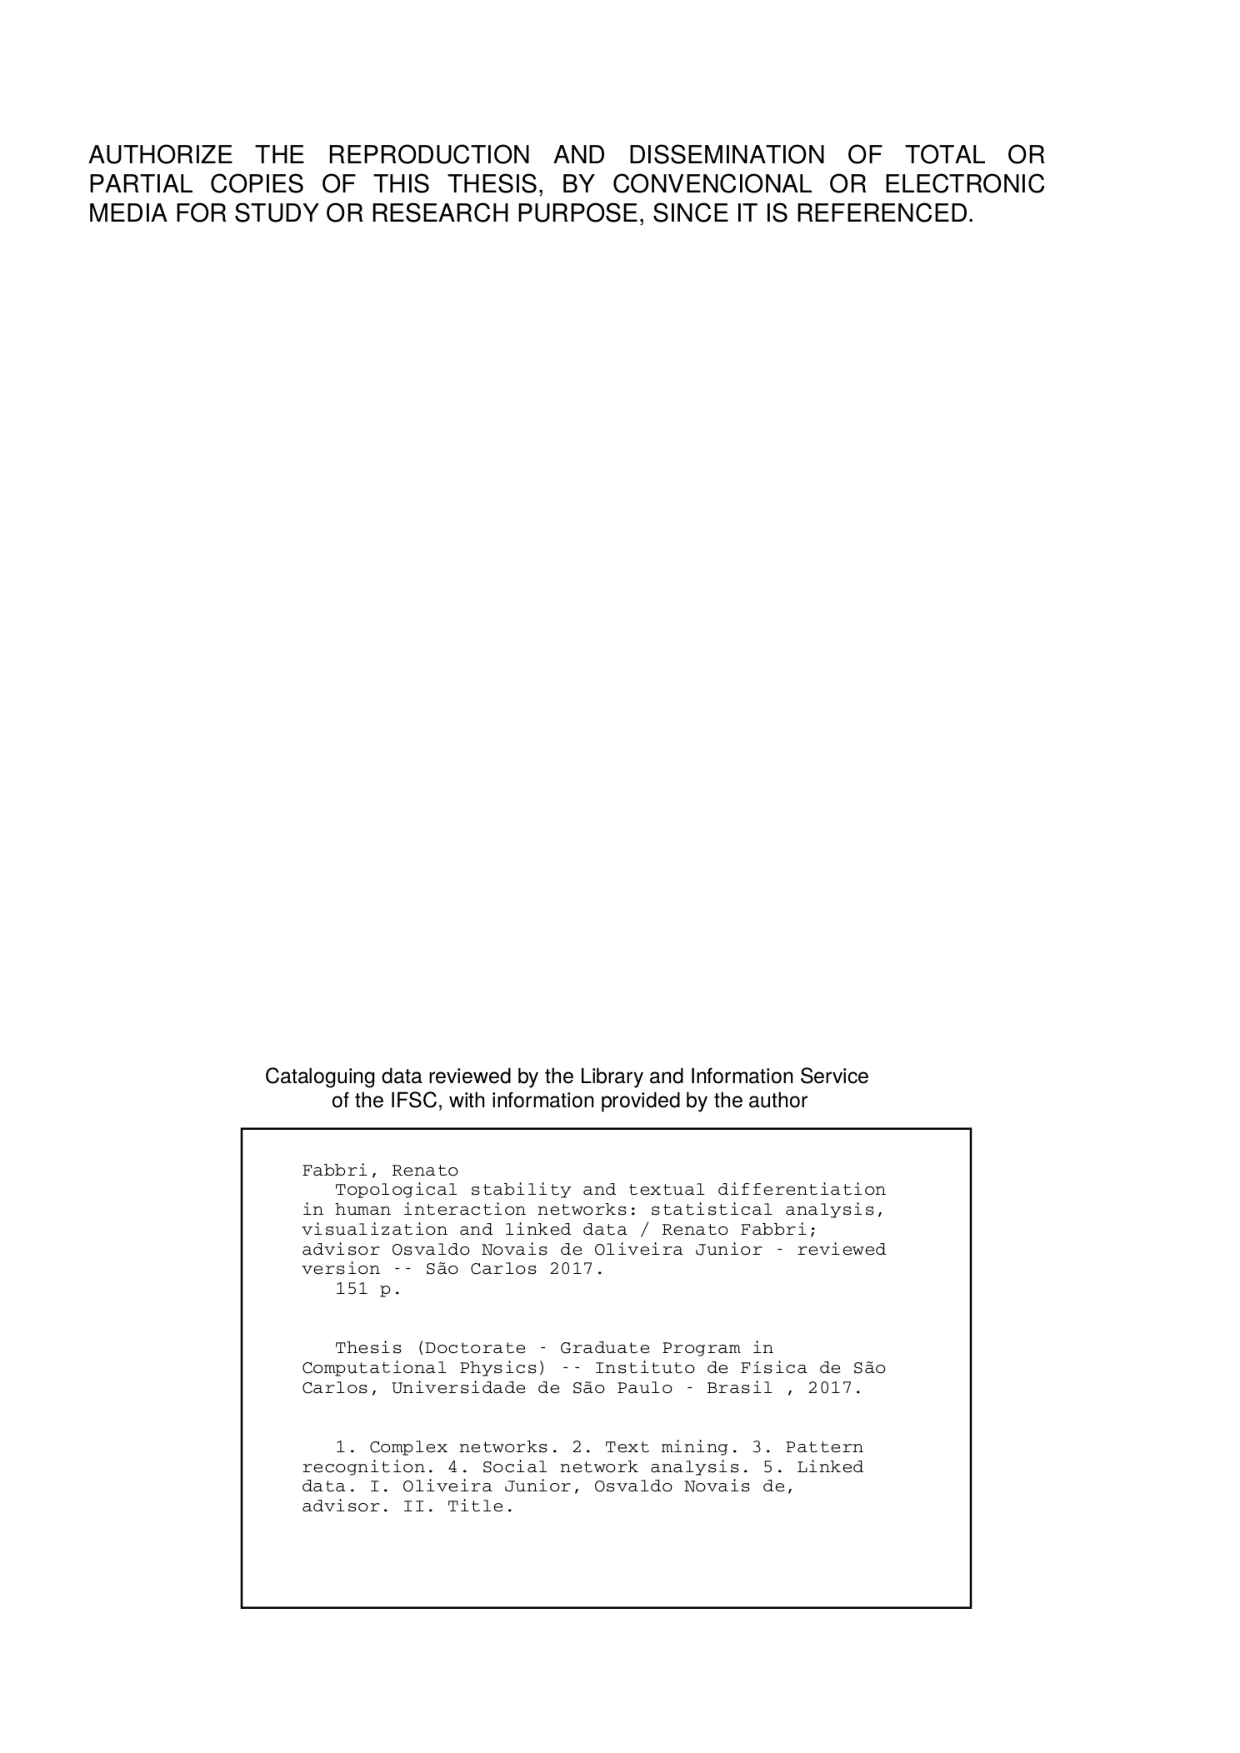
\includepdf{fichacatalografica___.pdf}
\end{fichacatalografica}
% Se você optar por elaborar a ficha catalográfica, deverá 
% incluir uma % antes das 3 linhas acima e tirar a % antes
% do comando % ---
% Inserir a ficha bibliografica
% ---
% Isto é um exemplo de Ficha Catalográfica, ou ``Dados internacionais de
% catalogação-na-publicação''. Você pode utilizar este modelo como referência. 
% Porém, provavelmente a biblioteca da sua universidade lhe fornecerá um PDF
% com a ficha catalográfica definitiva após a defesa do trabalho. Quando estiver
% com o documento, salve-o como PDF no diretório do seu projeto e substitua todo
% o conteúdo de implementação deste arquivo pelo comando abaixo:
%
\begin{fichacatalografica}
	\hspace{-1.4cm}
	\imprimirnotaautorizacao \\ \\
	%\sffamily
	\vspace*{\fill}					% Posição vertical
	\begin{center}					% Minipage Centralizado
		\imprimirnotabib \\
\begin{table}[htb]
	\scriptsize
	\centering	
	\begin{tabular}{|p{0.9cm} p{8.7cm}|}
		\hline
	      & \\
		  &	  \imprimirautorficha     \\
		
		 \imprimircutter & 
							\hspace{0.4cm}\imprimirtitulo~  / ~\imprimirautor~ ;  ~\imprimirorientadorcorpoficha. -- 	\imprimirlocal, \imprimirdata.   \\
		
		  &  % Para incluir nota referente à versão corrigida no corpo da ficha,
			  % incluir % no início da linha acima e tirar a % do início da linha abaixo
			  %	\hspace{0.4cm} \imprimirtitulo~  / ~\imprimirautor~ ; ~\imprimirorientadorcorpoficha~- ~\imprimirnotafolharosto. -- \imprimirlocal, \imprimirdata.  \\
		
			\hspace{0.4cm}\pageref{LastPage} p. : il. (algumas color.) ; 30 cm.\\ 
		  & \\
		  & 
		    \hspace{0.4cm}\imprimirnotaficha ~--~ 
						  \imprimirunidademin, 
						  \imprimiruniversidademin, 
		                  \imprimirdata. \\ 
		  & \\                 
		   % Para incluir nota referente à versão corrigida em notas,
		    % incluir uma % no início da linha acima e	
		    % tirar a % do início da linha abaixo
		    % & \hspace{0.4cm}\imprimirnotafolharosto \\ 
		  & \\ 
		  & \hspace{0.4cm}1. LaTeX. 2. abnTeX. 3. Classe USPSC. 4. Editoração de texto. 5. Normalização da documentação. 6. Tese. 7. Dissertação. 8. Documentos (elaboração). 9. Documentos eletrônicos. I. \imprimirorientadorficha. 
		   II. Título. \\
	
		     %Se houver co-orientador, inclua % antes da linha (antes de II. Título.) 
		     %          e tire a % antes do comando abaixo 
		     %III. Título. \\   
		  \hline
	\end{tabular}
\end{table}
	\end{center}
\end{fichacatalografica}
% ---


%% ---
% Inserir a ficha bibliografica
% ---
% Isto é um exemplo de Ficha Catalográfica, ou ``Dados internacionais de
% catalogação-na-publicação''. Você pode utilizar este modelo como referência. 
% Porém, provavelmente a biblioteca da sua universidade lhe fornecerá um PDF
% com a ficha catalográfica definitiva após a defesa do trabalho. Quando estiver
% com o documento, salve-o como PDF no diretório do seu projeto e substitua todo
% o conteúdo de implementação deste arquivo pelo comando abaixo:
%
\begin{fichacatalografica}
	\hspace{-1.4cm}
	\imprimirnotaautorizacao \\ \\
	%\sffamily
	\vspace*{\fill}					% Posição vertical
	\begin{center}					% Minipage Centralizado
		\imprimirnotabib \\
\begin{table}[htb]
	\scriptsize
	\centering	
	\begin{tabular}{|p{0.9cm} p{8.7cm}|}
		\hline
	      & \\
		  &	  \imprimirautorficha     \\
		
		 \imprimircutter & 
							\hspace{0.4cm}\imprimirtitulo~  / ~\imprimirautor~ ;  ~\imprimirorientadorcorpoficha. -- 	\imprimirlocal, \imprimirdata.   \\
		
		  &  % Para incluir nota referente à versão corrigida no corpo da ficha,
			  % incluir % no início da linha acima e tirar a % do início da linha abaixo
			  %	\hspace{0.4cm} \imprimirtitulo~  / ~\imprimirautor~ ; ~\imprimirorientadorcorpoficha~- ~\imprimirnotafolharosto. -- \imprimirlocal, \imprimirdata.  \\
		
			\hspace{0.4cm}\pageref{LastPage} p. : il. (algumas color.) ; 30 cm.\\ 
		  & \\
		  & 
		    \hspace{0.4cm}\imprimirnotaficha ~--~ 
						  \imprimirunidademin, 
						  \imprimiruniversidademin, 
		                  \imprimirdata. \\ 
		  & \\                 
		   % Para incluir nota referente à versão corrigida em notas,
		    % incluir uma % no início da linha acima e	
		    % tirar a % do início da linha abaixo
		    % & \hspace{0.4cm}\imprimirnotafolharosto \\ 
		  & \\ 
		  & \hspace{0.4cm}1. LaTeX. 2. abnTeX. 3. Classe USPSC. 4. Editoração de texto. 5. Normalização da documentação. 6. Tese. 7. Dissertação. 8. Documentos (elaboração). 9. Documentos eletrônicos. I. \imprimirorientadorficha. 
		   II. Título. \\
	
		     %Se houver co-orientador, inclua % antes da linha (antes de II. Título.) 
		     %          e tire a % antes do comando abaixo 
		     %III. Título. \\   
		  \hline
	\end{tabular}
\end{table}
	\end{center}
\end{fichacatalografica}
% ---


% As informações que compõem a ficha catalográfica estão 
% definidos no arquivo USPSC-pre-textual-UUUU.tex
% ---


% ---
% Inserir errata
% ---

% \begin{errata}
% 	\OnehalfSpacing 			
% 	A errata é um elemento opcional, que consiste de uma lista de erros da obra, precedidos pelas folhas e linhas onde eles ocorrem e seguidos pelas correções correspondentes. Deve ser inserida logo após a folha de rosto e conter a referência do trabalho para facilitar sua identificação, conforme a ABNT NBR 14724. \cite{nbr14724}.
% 	
% 	Modelo de Errata:
% 		
% 	\begin{flushleft}\footnotesize 
% 			\setlength{\absparsep}{0pt} % ajusta o espaçamento da referência	
% 			\SingleSpacing 
% 			\imprimirautorabr~ ~\textbf{\imprimirtitulo}.	\imprimirdata. \pageref{LastPage}p. 
% 			%Substitua p. por f. quando utilizar oneside em \documentclass
% 			%\pageref{LastPage}f.
% 			\imprimirtipotrabalho~-~\imprimirinstituicao, \imprimirlocal, \imprimirdata. 
%  	\end{flushleft}
% \vspace{\onelineskip}
% \OnehalfSpacing 
% \center
% \textbf{ERRATA}
% \vspace{\onelineskip}
% \OnehalfSpacing 
% \begin{table}[htb]
% 	\center
% 	\footnotesize
% 	\begin{tabular}{p{1.4cm} p{1cm} p{3cm} p{3cm} }
% 		\hline
% 		\textbf{Folha} & \textbf{Linha}  & \textbf{Onde se lê}  & \textbf{Leia-se}  \\
% 			\hline
% 			1 & 10 & auto-conclavo & autoconclavo\\
% 		\hline
% 	\end{tabular}
% \end{table}
% 
% 
% \end{errata}
% ---

% ---
% Inserir folha de aprovação
% ---

% A Folha de aprovação é um elemento obrigatório da NBR 4724/2011 (seção 4.2.1.3). 
% Após a defesa/aprovação do trabalho, gere o arquivo folhadeaprovacao.pdf da página assinada pela banca 
% e iclua o arquivo utilizando o comando abaixo:
% \includepdf{folhadeaprovacao.pdf}
% 
\includepdf{PaginaEmBranco.pdf}

% Alternativa para a Folha de Aprovação:
% Se for a sua opção elaborar uma folha de aprovação, insira uma % antes do comando acima que inclui o arquivo folhadeaprovacao.pdf,
% tire o % do comando abaixo e altere o arquivo folhadeaprovacao.tex conforme suas necessidades
%\include{folhadeaprovacao}

% 
\includepdf{PaginaEmBranco.pdf}

% ---
% Dedicatória
% ---
\begin{dedicatoria}
   \vspace*{\fill}
   \centering
   \noindent
%   \textit{ Este trabalho é dedicado à Deus e à minha família.} \vspace*{\fill}
   \textit{ This work is dedicated to God and my family, whose constant support made it possible.} \vspace*{\fill}
\end{dedicatoria}
% ---

% ---
% Agradecimentos
% ---=====
\begin{agradecimentos}
I thank my advisor
Prof. Dr. Osvaldo Novais de Oliveira Junior
for his patience and prompt responses.	
I thank Prof. Dr. Luciano da Fontoura Costa
whose research also inspired this thesis
and for introducing me to complex networks.
I thank Prof. Dr. Leonardo Paulo Maia for important discussions regarding statistics and
written discourse.
I thank the Institute of Advanced Studies (IEA/USP)
for enabling me to receive guest researchers and hosting meetings in the years of 2013 and 2014.
I thank Prof. Dr. Yvonne Primerano Mascarenhas (IFSC/USP) for her time in articulating with the IEA.
I thank Prof. Dr. Dilvan de Abreu Moreira (ICMC/USP) for guiding me in understanding linked data/semantic web.
I thank the members of the São Carlos Institute of Physics,
including the instructors, the administration and the secretariat
for the mindfulness and patience whenever I needed to reach them.

	I thank the Brazilian Presidency and the United Nations Development Program (UNDP) for
the partnership established with this research in the year of 2014 (consulting contract 2013/00056, project BRA/12/018).
I thank Ricardo Poppi for his time, experience and mentoring while he was the general coordinator of new media of the Brazilian Presidency.
	I thank the Military from the Brazilian Army Prof. Ronald Emerson Scherolt da Costa for assisting the mentorship.
	I thanks Fabricio Solagna, Grazielle Machado, Ana Célia Costa,
	Joenio Marques da Costa, Daniela Feitosa, Prof. Dr. Paulo Meirelles (UnB), Prof. Dr. Fernando William Cruz (UnB), Antonio Carlos Wosgrau,
	Cintia Cinquini, Anjuli Tostes Faria Osterne and Prof. Dr. Frederick van Amstel (UFPR) for
a series of occasions in which I had the opportunity to learn and maybe contribute to State affairs
regarding interfaces with the civil society and the introduction of scientific knowledge and technologies.
I thank the government and State specialists and authorities for the interviews in which they
allowed me to formalize conceptualizations of social participation instances and mechanisms:
conference, forum, council, ombudsman, public consultation, dialog table, monitoring table.
	Namely, I thank Pedro Pontual, Dra. Maria Carmen Romcy de Carvalho (Biblioteca Digital de Participação Social - PR), Prof. Dr. Fernando Cruz, Clovis Souza, Paula Pompeu, Lígia Maria Alves Pereira,
Valéssio Brito, Fernanda Lobato, Fabiano Rangel, Anjuli Osterne and Paulo Guimarães.
Some of the input was obtained in a workshop held by the presidency,
reason why I don't have the full name of the following contributors
which I also thank: Silvia, Roberto and Márcia.

I thank the Nexos research network for the precious support in deepening concepts related
to the study of human individuals and groups.
A special thanks here goes to the philosopher Prof. Dr. Marília Mello Pisani (CCNH/UFABC) and the social psychologist 
	Prof. Dr. Deborah Christina Antunes (Psychology Course/UFC/Sobral Campus).
I also thank the anthropologist Prof. Dr. Massimo Canevacci (Università di Roma "La Sapienza" and IEA/USP)
for his presence and tolerance in meetings and artistic presentations.

I thank the labMacambira.sf.net collective for numerous discussions and guidance
concerning free and digital culture.
Namely, I thank Prof. Dr. Ricardo Fabbri (IPRJ/UERJ), Vilson Vieira da Silva Junior, Daniel Penalva, Caleb Mascarenhas Luporini, Danilo Shiga,
Dr. Antonio Pessotti, Guilherme Lunhani, Geraldo Magela de Castro Rocha Junior and Dr. Carlos Lobo for insights and fruitful discussions.
I thank the architect and cultural activist Daniel Marostegan e Carneiro for his invaluable support in
the foundation of the labMacambira.sf.net and in the advancement of digital culture conceptualizations.
I thank the Ethymos company and the cultural center Teia Casa de Criação/Pontão Nós Digitais for hosting experiments, webpages, bots and documents in their online infrastructure for years.
I thank João Paulo Mehl, Marco Antonio Konopacki and Jacson Passold for their time, patience and trust in allowing me to benefit from the facilities of Ethymos.

I thank the Metareciclagem network for enabling me to start this research by proposing
a study about the ``end of the world''.
	Special thanks here goes to Prof. Guilherme Rafael (Glerm) Soares (CECULT/UFRB), Simone Bittencourt and Adriano Belisário
for sharing their time and understandings.
I distinctively admire and benefit from what Prof. Glerm yields.

I thank the linguist Dr. Chandra Wood Viegas for her stimulant interest
which culminated in collaborations and citations of preliminary results of this research in her doctorate thesis
	about the indigenous Kokama culture.

I thank my family for the invaluable support in every step.
I thank my parents, the mathematician Cláudia Maria Costa Lopes (teaches at Petrópolis/RJ) and the
physicist Prof. Dr. Maurício Fabbri (LAS/INPE and USF), for the good education that
allowed me to strive in a number of fields of knowledge 
and develop technological, social and artistic artifacts.
I also thank my stepfather, the biophysicist Prof. Dr. Francisco José Pereira Lopes (UFRJ),
for his time in a number of discussions.
I value exceptionally the influence my brother Prof. Dr. Ricardo Fabbri (IPRJ/UERJ)
has in my current appreciation
of the sciences and the academia and computer technologies.
He encouraged me for decades to pursue a deeper background and believed in my ability to acquire and yield knowledge.

I thank the National Counsel of Technological and Scientific Development (CNPq)
for the financial support (140860/2013-4, project 870336/1997-5).
I thank and admire the researchers that keep their works freely available online,
specially those who make video lectures e.g. on Coursera, edX and Complexity Explorer (Santa Fe Institute).
I thank the open source and free software communities for sharing their work,
which made possible the developments presented in this thesis.
% SGPR, PNUD
% labmacambira
% wife and family
% O Grupo desenvolvedor do Pacote USPSC, atualmente composto da Classe USPSC e do  Modelo para teses e dissertações em \LaTeX\ utilizando a classe USPSC, agradece especialmente ao Luis Olmes, doutorando do Instituto de Ciências Matemáticas e de Computação (ICMC) da Universidade de São Paulo (USP), pelas primeiras orientações sobre o \LaTeX\ .
% 
% Agradecemos ao Lauro César Araujo pelo desenvolvimento da classe  \abnTeX, modelos canônicos e tantas outras contribuições que nos permitiu o desenvolvimento da classe USPSC e seus modelos.
% 
% Os nossos agradecimentos aos integrantes do primeiro
% projeto abn\TeX\, Gerald Weber, Miguel Frasson, Leslie H. Watter, Bruno Parente Lima, Flávio de Vasconcellos Corrêa, Otavio Real
% Salvador, Renato Machnievscz, e a todos que contribuíram para que a produção de trabalhos acadêmicos em conformidade com
% as normas ABNT com \LaTeX\ fosse possível.
% 
% Agradecemos ao grupo de usuários
% \emph{latex-br}{\url{http://groups.google.com/group/latex-br}}, aos integrantes do grupo
% \emph{\abnTeX}{\url{http://groups.google.com/group/abntex2}  e \url{http://www.abntex.net.br/}}~que contribuem para a evolução do \abnTeX.
\end{agradecimentos}
% ---

% ---
% Epígrafe
% ---
\begin{epigrafe}
    \vspace*{\fill}
	\begin{flushright}
		% \textit{``The heart of the discerning acquires knowledge, \\
		% for the ears of the wise seek it out.''\\
		% Proverbs 18:15}
		\textit{``Call to me and I will answer you and tell you\\
		great and unsearchable things you do not know.''\\
		Jeremiah 33:3}
	\end{flushright}
\end{epigrafe}
% ---


% ---
% Abstract
% ---
\autor{Fabbri, R.}
\begin{resumo}[Abstract]
	\begin{flushleft}\footnotesize 
		\setlength{\absparsep}{0pt} % ajusta o espaçamento dos parágrafos do resumo		
 		\SingleSpacing 
 		\imprimirautorabr~ ~\textbf{\imprimirtitleabstract}.	\imprimirdata.  \pageref{LastPage}p. 
		%Substitua p. por f. quando utilizar oneside em \documentclass
		%\pageref{LastPage}f.
		\imprimirtipotrabalho~-~\imprimirinstituicao, \imprimirlocal, 	\imprimirdata. 
 	\end{flushleft}
	\OnehalfSpacing 
	 This work reports on stable (or invariant) topological properties and textual differentiation in human interaction networks,
	 with benchmarks derived from public email lists.
	 Activity along time and topology were observed in snapshots in a timeline, and at
	 different scales. Our analysis shows that activity is practically the same for all networks across timescales
	 ranging from seconds to months. The principal components of the participants in the topological metrics
	 space remain practically unchanged as different sets of messages are considered.
	 The activity of participants
	 follows the expected scale-free outline, thus yielding the hub, intermediary and peripheral classes of vertices by
	 comparison against the Erdös-Rényi model.
	 The relative sizes of these three sectors are essentially the same
	 for all email lists and the same along time.
	 Typically, 3-12\% of the vertices are hubs, 15-45\% are intermediary
	 and 44-81\% are peripheral vertices.
	 Texts from each of such sectors are shown to be very different through direct measurements and through an adaptation of the Kolmogorov-Smirnov test.
	 These properties are consistent with the literature and may be general for human
	 interaction networks, which has important implications for establishing a typology of participants based on
	 quantitative criteria.
	 For guiding and supporting this research, we also developed a visualization method of dynamic networks through animations.
	 To facilitate verification and further steps in the analyses, we supply a linked data representation of data related to our results.
   \vspace{\onelineskip}
 
   \noindent 
   \textbf{Keywords}: Complex networks. Text mining. Pattern recognition. Social network analysis. Linked data.
\end{resumo}

% ---
% Resumo
% ---
% Se o idioma do texto for em inglês, o abstract deve preceder o resumo
% resumo em português
\setlength{\absparsep}{18pt} % ajusta o espaçamento dos parágrafos do resumo		
\titulo{Estabilidade topológica e diferenciação textual em redes de interação humana: análise estatística, visualização e dados ligados}
     	\tipotrabalho{Tese (Doutorado em Ci\^encias)}
        \area{F\'isica Aplicada}
        \opcao{F\'isica Computacional}
\begin{resumo}[Resumo]
 \begin{otherlanguage*}{portuguese}
	\begin{flushleft}\footnotesize 
			\setlength{\absparsep}{0pt} % ajusta o espaçamento da referência	
			\SingleSpacing 
			\imprimirautorabr~ ~\textbf{\imprimirtitulo}.	\imprimirdata. \pageref{LastPage}p. 
			%Substitua p. por f. quando utilizar oneside em \documentclass
			%\pageref{LastPage}f.
			\imprimirtipotrabalho~-~\imprimirinstituicao, \imprimirlocal, \imprimirdata. 
 	\end{flushleft}
\OnehalfSpacing 			
	 Este trabalho relata propriedades topológicas estáveis (ou invariantes) e diferenciação textual em redes de interação humana,
	 com referências derivadas de listas públicas de e-mail.
	 A atividade ao longo do tempo e a topologia foram observadas em instantâneos ao longo de uma linha do tempo e em
	 diferentes escalas.
	 A análise mostra que a atividade é praticamente a mesma para todas as redes em escalas temporais
	 de segundos a meses.
	 As componentes principais dos participantes no espaço das métricas topológicas
	 mantêm-se praticamente inalteradas quando diferentes conjuntos de mensagens são considerados.
	 A atividade dos participantes
	 segue o esperado perfil livre de escala, produzindo, assim, as classes de vértices dos hubs, dos intermediários e dos periféricos em
	 comparação com o modelo Erdös-Rényi.
	 Os tamanhos relativos destes três setores são essencialmente os mesmos
	 para todas as listas de e-mail e ao longo do tempo.
	 Normalmente, 3-12\% dos vértices são hubs, 15-45\% são intermediários
	 e 44-81\% são vértices periféricos.
	 Os textos de cada um destes setores são considerados muito diferentes através de uma adaptação dos testes de Kolmogorov-Smirnov.
	 Estas propriedades são consistentes com a literatura e podem ser gerais para
	 redes de interação humana, o que tem implicações importantes para o estabelecimento de uma tipologia dos participantes com base em
	 critérios quantitativos.
	 De modo a guiar e apoiar esta pesquisa, também desenvolvemos um método de visualização para redes dinâmicas através de animações.
	 Para facilitar a verificação e passos seguintes nas análises, fornecemos uma representação em dados ligados dos dados relacionados aos nossos resultados.

 \textbf{Palavras-chave}: Redes complexas. Mineração de texto. Reconhecimento de padrões. Análise de redes sociais. Dados ligados.
 \end{otherlanguage*}
\end{resumo}


% ---
% inserir lista de ilustrações
% ---
\pdfbookmark[0]{\listfigurename}{lof}
\listoffigures*
\cleardoublepage
% ---

% ---
% inserir lista de tabelas
% ---
\pdfbookmark[0]{\listtablename}{lot}
\listoftables*
\cleardoublepage
% ---

% ---
% inserir lista de quadros
% ---
% \pdfbookmark[0]{\listofquadroname}{loq}
% \listofquadro*
% \cleardoublepage
% ---

% ---
% inserir lista de abreviaturas e siglas
% ---
\begin{siglas}
	\item[AA] Algorithmic Autoregulation
	\item[HTML] HyperText Markup Language
	\item[HTTP] HyperText Transfer Protocol
	\item[IRC] Internet Relay Chat
	\item[LOSD] Linked Open Social Database
	\item[PCA] Principal Component Analysis
	\item[POS] Part-Of-Speech
	\item[RDF] Resource Description Framework
	\item[SPARQL] SPARQL Protocol and RDF Query Language
	\item[URI] Uniform Resource Identifier
	\item[Versinus] Line and sine (Latin versus+sinus) layout for graph visualization.
	\item[W3C] World Wide Web Consortium
\end{siglas}
% \begin{siglas}
%     \item[ABNT] Associação Brasileira de Normas Técnicas
%     \item[abnTeX] ABsurdas Normas para TeX
% 	\item[EESC] Escola de Engenharia de São Carlos
% 	\item[IAU] Instituto de Arquitetura e Urbanismo
% 	\item[IBGE] Instituto Brasileiro de Geografia e Estatística
% 	\item[ICMC] Instituto de Ciências Matemáticas e de Computação
% 	\item[IFSC] Instituto de Física de São Carlos
% 	\item[IQSC] Instituto de Química de São Carlos
% 	\item[USP] Universidade de São Paulo
% 	\item[USPSC] Campus USP de São Carlos
% 	
% \end{siglas}
% ---

% ---
% inserir lista de símbolos
% ---
% \begin{simbolos}
%   \item[$ \Gamma $] Letra grega Gama
%   \item[$ \Lambda $] Lambda
%   \item[$ \zeta $] Letra grega minúscula zeta
%   \item[$ \in $] Pertence
% \end{simbolos}
% ---
% ---
% inserir o sumario
% ---
\pdfbookmark[0]{\contentsname}{toc}
\tableofcontents*
\cleardoublepage
% ---
% ----------------------------------------------------------
% ELEMENTOS TEXTUAIS
% ----------------------------------------------------------
\textual
% Os capítulos são inseridos como arquivos externos 

% Capítulo 1 - Introdução
% ---
%% USPSC-Introducao.tex
% ----------------------------------------------------------
% Introdução (exemplo de capítulo sem numeração, mas presente no Sumário)
% ----------------------------------------------------------
% \chapter[Introdução]{Introdução}
\chapter{Introduction}\label{ch:int}
The first studies dealing explicitly with human interaction networks
date from the nineteenth century while the foundation of
social network analysis is generally attributed to the psychiatrist Jacob Moreno in mid twentieth century~\cite{moreno,newmanBook}.
With the increasing availability of data related to human interactions, research about these networks has grown continuously.
Contributions can now be found in a variety of fields, from social sciences and humanities~\cite{latour2013} to computer science~\cite{bird} and physics~\cite{barabasiHumanDyn,newmanFriendship}, given the multidisciplinary nature of the topic.
One of the approaches from an exact science perspective is to represent interaction networks as complex networks~\cite{barabasiHumanDyn,newmanFriendship}, with which 
several features of human interaction have been revealed.
For example, the topology of human interaction networks exhibits a scale-free outline,
which points to the existence of a small number of highly connected hubs and a large number of poorly connected nodes.
The dynamics of complex networks representing human interaction has also been addressed~\cite{barabasiEvo,newmanEvolving}, but only to a limited extent, since research is normally focused on a particular metric or task, such as accessibility or community detection~\cite{access,newmanModularity}. 





There are numerous articles, books, websites and software tools about complex and social networks and about text mining in social media.
There are fewer endeavours to characterize these networks beyond general features such as the scale-free 
aspect or to deal with text produced by social networks from the complex networks background.
Research on network evolution is often restricted to network growth, in which there is a monotonic increase in the number of events~\cite{barabasiEvo}.
Network types have been discussed with regard to the number of participants, intermittence of their activity and network longevity~\cite{barabasiEvo}. Two topologically different networks emerged from human interaction networks, depending on whether the frequency of interactions follows a generalized power law or an exponential connectivity distribution~\cite{barabasiTopologicalEv}. In email list networks, scale-free properties were reported with $\alpha \approx 1.8$~\cite{bird} (as in web browsing and library loans~\cite{barabasiHumanDyn}), and different linguistic traces were related to weak and strong ties~\cite{Gmane2}.

In this thesis, e-mail lists were chosen to represent human interaction networks, which were analyzed according to two broad aspects: the possible stability of the topology of the networks and the linguistic usage of distinct types of participants in the network. In the analysis, the topology of the networks was studied with regard to well-established topological metrics and well-established networks models. The text of the networks was studied with regard to statistics derived from the strings and from syntactics and semantics.
The fact that unreciprocated edges often exceed 50\% in human interaction networks~\cite{newmanEvolving} motivated the inclusion of symmetry metrics in our analysis. 
No correlation of topological characteristics and geographical coordinates was found~\cite{barabasiGeo},
therefore geographical positions were not considered in our study.
Gender related behavior in mobile phone datasets was indeed reported~\cite{barabasiSex}
but it is not relevant for the present work because email messages and addresses have no gender related metadata~\cite{gmanePack}. As for the language usage in the networks, emphasis was given to statistical features of the text such as number of tokens and known words, sizes of tokens, known words, sentences and messages. 
Statistics were also derived from syntactics through POS tags (e.g. nouns, adjectives, verbs) and semantics through Wordnet synsets.

The remainder of this chapter provides some background knowledge relevant to the topics discussed in the thesis, especially complex networks, text mining, graph visualization and linked data. In Chapter 2, the data and methods where described while the results and discussion are in Chapter~\ref{ch:disc}. 
Conclusions and further work are stated in Chapter~\ref{ch:concl}.
The appendices bring further results from this research.


\section{Related knowledge}
\subsection{Complex networks}
Although not universally accepted, it is commonplace to define a complex network to be
a ``graph with non-trivial topological features''~\cite{newmanBook}.
We might add to this definition that a complex network is also a large graph (even though no consensus appears to exist as 
to what \emph{large} means in this context)
and that it is a graph representation of a system found in natural, real or empirical system.
Another way to approach the definition of ``complex networks'' is to define it as
complex systems modeled as networks.
This second definition is also useful but is even more problematic as
there is no consensus of what a \emph{complex system} is.
Even so, one should keep in mind that authors often define a complex system
to be a system composed with many parts in which ``the whole is more than
the sum of its parts''.
Authors also often consider complex systems to have capabilities
to ``process information'', to adapt and to reproduce~\cite{complexity}.

A graph is a structure that consists of a set of objects (called vertices)
and a set of binary/dual relations of the objects (called edges).
A graph might be unweighted and undirected (the simplest possibility),
weighted and undirected, unweighted and directed, or weighted and directed.

The most usual representations of graphs (and networks) are the matrix, list and node-edge representations.
In the matrix representation, each entry $a_{ij}$ is non-zero if $i$ is linked to $j$;
entries might be other than 0 and 1 in weighted graphs; undirected graphs yield symmetric matrices.
There are two common list representations of graphs, one lists each pair of vertices that are connected,
the other holds a list for each vertex in which are all the vertices connected to it (a list of lists).
In the node-edge representation, each node is represented as a point while each edge is represented
by a line between corresponding nodes.
The matrix representation is essential for algebraic reasoning and for deriving metrics
while the node-edge representation is important for illustration and intuitive guidance
in characterizing the systems.

\subsubsection{A good justification for applying the complex networks theory}
The estimated number of atoms in the universe, often used as a reference of largeness,
is $\approx 10^{80}$.
Let us find the number of vertices needed to reach such number of possible networks.
Consider the simplest case of the unweighted and undirected networks.
Each edge can exist or not (i.e. it is a Bernoulli variable) and with $n$ vertices there are
at most ${n \choose 2}$ edges.
Therefore:
\begin{align}
2^{n \choose 2} > 10^{80} \Rightarrow 
log_2[2^{n \choose 2}] > log_2(10^{80}) \Rightarrow
{n \choose 2} > \frac{log_{10}(10^{80})}{log_{10}2} \Rightarrow \nonumber\\
\Rightarrow \frac{n.(n-1)}{2} > \frac{80}{log_{10}2} \Rightarrow
N > 23,5988 \;\;\;\;\;\;\;\;\;\;\;\;\;\;\;\;\;\;\;\;\;
\nonumber
\end{align}
That is, with only 24 vertices we have more possible networks than
the estimated number of atoms in the universe.
We should also add that the number of possible networks grows
very fast with the number of vertices.
This is a good reason for characterizing such systems by means
of paradigmatic networks and generic metrics for nodes and the network (and edges, but it is less often).

\subsubsection{Basic metrics}\label{se:intMea}
Section~\ref{measures} gives a mathematical account of the following metrics,
which are used here for characterizing basic types
of networks in the next section.
Such metrics are:
\begin{itemize}
\item Degree $k_i$: number of edges linked to vertex $i$.
\item In-degree $k_i^{in}$: number of edges ending at vertex $i$.
\item Out-degree $k_i^{out}$: number of edges departing from vertex $i$.
\item Strength $s_i$: sum of weights of all edges linked to vertex $i$.
\item In-strength $s_i^{in}$: sum of weights of all edges ending at vertex $i$.
\item Out-strength $s_i^{out}$: sum of weights of all edges departing from vertex $i$.
\item Betweenness centrality $bt_i$: fraction of geodesics that contain vertex $i$.
\item Clustering coefficient $cc_i$: fraction of pairs of neighbors of $i$ that are linked, i.e. the standard clustering coefficient metric for undirected graphs.
\end{itemize}
% distance between vertices
In the following discussion, we also use the concept of distance between a pair of nodes,
which is the number of edges between the nodes.

\subsubsection{Basic types of networks}
Complex networks are often characterized in terms of paradigmatic models.
There are diverse models, but we can glimpse the background theory
with the following ones~\cite{luMeasures}:
\begin{itemize}
\item The Erdös-Rényi model\footnote{This name is also used for the model in which, for a fixed number of nodes and a fixed number of links, all networks are equally likely. This is the model originally introduced by Paul Erdös and Alfréd Rényi~\cite{erdosOrig}.
We choose the definition given in the main text, which is closely related to the one given in this footnote, because it is more commonly used nowadays.}: each pair of nodes is connected with a fixed random probability $p$.
This model presents a characteristic degree ($n.p$ where $n$ is the number of nodes), low clustering and low average distance between nodes.
\item Spatial network, also called geographic network or geometric graph: nodes are located in a metric space and the probability that two nodes are connected is greater as the distance between nodes gets smaller. These networks present characteristic degrees, high clustering and large average distance between nodes.
\item Small-word network: defined as a network where the typical distance between nodes grows with the logarithm of the number of nodes while the average clustering coefficient is not small (larger than e.g. in the Erdös-Rényi model).
One method for constructing a small-world network is to start with a regular lattice in which each node is connected to $k$ nearest neighbors.
Each link is then rewired with probability $p$.
With intermediate values of $p$ such as $0.01<p<0.1$, we obtain a network with both short average distance between nodes (as in the Erdös-Rényi model) and a high average clustering coefficient (as in the spatial network).
This model presents a characteristic degree.
\item Scale-free networks: in which the degree distribution $p(k)$ follows a power law ($p(k)=C.k^{-\alpha}$ where $C$ and $\alpha$ are constants).
These networks are qualitatively characterized by the presence of a large number of poorly connected and of few highly connected hubs.
Important is the absence of a characteristic degree, thus the name 'scale-free network'.
\item Other networks: among important models of networks are exponential networks, networks with community structure and hybrid models.
\end{itemize}
Real networks most often exhibit scale-free and small-world properties.
This is the case of most e.g. social, gene and food networks.
However, one should be cautious about such statement because
the networks derived from the real systems depend heavily
in what is considered a node and a link,
i.e. on how the system is modeled as a graph.
Another noteworthy remark is that
the Erdös-Rényi networks, i.e. graphs of the Erdös-Rényi model, are frequently pin-pointed as the networks with trivial
topological properties.
This model is considered as a paradigmatic ``complex network'', concept often defined as graphs with non-trivial topological properties,
which is a contradiction. Therefore, the term complex networks is not a very well defined notion, as it occurs for the \emph{complexity theory} in general.


\subsection{Text mining of social data}
Text mining is a multidisciplinary field,
it is an extension of data mining to (often unstructured) textual data
with the goal of discovering structure and meaning~\cite{customText}.
A general outline of a text mining endeavor involves structuring input text,
deriving patterns and the evaluation of the output.
There are actually numerous models of such outline,
as e.g. considering document collection and obtaining a final report in the
start and end respectively~\cite{textSurvey}.
Text mining tasks include document summarization, sentiment analysis
and natural language processing techniques such as part of speech tagging~\cite{ntlk}.
Among the applications one may include social media monitoring, automated ad placement, and development of tools for 
semantics ~\cite{textSurvey}.
It is believed that applying text mining to social media
can yield interesting findings in human behavior~\cite{customText}.
Although there is no clear cut, text mining is sometimes divided into linguistic and non-linguistic~\cite{customText}.
In the first case, techniques borrowed from linguistics are present, such as
the analysis of discourse and part of speech tagging,
and it is often mingled with natural language processing or computational linguistics (see Section~\ref{amb} for a coherent distinction of the fields).
In the non-linguistic text mining, text is analyzed by means of statistical features
derived from e.g. the size of tokens and sentences,
and might be more easily related to the intuitive concept of data mining of text.
In this thesis we use both perspectives.

\subsection{Visualization of static and dynamic graphs}
Static graph visualization is achieved in many ways,
most usually through the node-link (often called network diagram)
and matrix representations.
Representing graphs as node-link diagrams has a long tradition which goes back 
at least to the works of Ramon Llull in the 13th century~\cite{llull}.
To glimpse at the theory involved in visualizing networks~\cite{eades}, we mention three aspects:
\begin{itemize}
\item criteria for the quality of layouts might include the number of crossing edges or the area of the drawing relative to the closest distance between two vertices.
\item Layout methods are derived e.g. by placing vertices in a circular fashion, by using the eigen vectors from a worked out variant of the adjacency matrix as coordinates, or by force-based methods. For large graphs, including a number of social networks, the force-based networks are reported as useful. Therefore, we illustrate this method with the simplest model we could find in the specialized literature. Let $f_a$ be the attraction force, $f_r$ is the repulsion force, $d$ is the distance between the vertices and $k$ is a constant. The model introduced by Fruchterman and Reingold~\cite{fr} defines the forces as:
\begin{align}
f_a = \frac{d^2}{k}\\
f_d = -\frac{k^2}{d}
\end{align}
On a computer software, one usually starts with a random layout and performs a number of iterations updating the position of nodes
using these forces to obtain the intended force-directed layout.
\item Graph drawings are often developed for specific applications e.g. in biology (as for protein and gene interactions), in social networks, in tree diagrams.
\end{itemize}

The core difference of dynamic graphs to static graphs is that vertices and edges
can be added and removed over time.
If we define the static graph G as $G:=(V,E)$ where V are the vertices as E are the edges in G,
a dynamic graph might be defined as $\Gamma:=(G_1,G_2,...,G_n)$ where $G_i:=(V_i,E_i)$
are static graphs and indices refer to a sequence of time steps $(t_1,t_2,...,t_n)$.
In dynamic graph visualization most usually graphs are represented as animated diagrams
or charts based on a timeline~\cite{dynGraph}.
In this thesis we make use of node-link diagrams of both static and dynamic graphs.

\subsection{Linked (open) data}
The fields of social network analysis and complex networks
are widely researched.
However, there is a lack of open datasets for benchmarking results,
especially associated with the complex networks field,
yielding diverse results from poorly related sources.
Recently, a myriad of results have been reported which are based on
diverse datasets most often not accessible to researchers other than the publishing authors.
In this thesis we present resources for having open databases to provide 
the scientific community with a friendly and common repertoire.
We chose to use the linked data technology and follow W3C best practices for publishing data.

Linked data refers to data published in the web in such a way that it is
machine readable and complies with a set of best practices.
The web of data is constructed with documents on the web 
such as the web of HTML documents.
In practice, the idea of linked data can me summarized
by 1) the use of RDF to publish data on the web and 2) the use of RDF
links to interlink data from different sources.
The web is expected to be interconnected and to grow by the systematic application of four
steps~\cite{lee1}:
\begin{itemize}
\item Use URIs to identify things~\cite{uri}.
\item Use HTTP URIs.
\item Provide useful information when an URI is accessed via HTTP.
\item Provide other URIs in the description of resources so human
and machine agents can perform discovery.
\end{itemize}

The Linked Open Data~\cite{lod} builds an ever growing cloud of data,
the global data space, which is usually
conceived as centered around the DBPedia, a linked data representation
of data from Wikipedia~\cite{dbpedia0,dbpedia}.

\subsubsection{RDF}
The Resource Description Framework (RDF), a W3C
recommendation, is a model for data
interchange.
It is based on the idea of making statements about resources in the form
of triples, i.e. expressions in the form ``subject - predicate -
object''.
RDF can be serialized in several file formats, including RDF/XML,
Turtle and Manchester, all of which, in essence, represent a labeled and
directed multi-graph.
RDF may be stored in a type of database referred to as a triplestore~\cite{rdf}.

As an example of an RDF statement, the following triple in the Turtle
format asserts that ``the paper has color white'':\\
\texttt{http://example.org/Things\#Paper http://example.org/hasColor\\
http://example.org/Colors\#White .}
% This work makes available an open database with diverse provenance and
% to furnish the scientific community with a friendly and common repertoire.

Integration and uniformity of access is obtained through linked data
representation, as explained in Section~\ref{queries}.

\subsection{Social participation}
A significant share of our endeavor was oriented towards social participation,
i.e. to facilitate civil engagement in a community, most significantly in State affairs.
More concretely, we published data from a social participation federal portal~\cite{losd},
applied complex networks and text mining criteria for resources recommendation~\cite{pnud3,pnud4,opa} and
proposed a ranking algorithm for voted proposals in another federal participation portal~\cite{dialogaAlg}.
Such works were performed within a United Nations Development Program consulting contract,
in partnership with the Brazilian Presidency of the Republic and published publicly mainly as technical reports~\cite{pnud3,pnud4,opa}.
This aspect of our research was important for maturing topics and understanding
the extent to which they are applied in pragmatic contexts.
It is left mostly as subsidiary documents in this thesis to allow for an easy public access.

\subsection{Other}
Given the multidisciplinary condition of our work and of the implied topics,
many other fields of knowledge could be further explored in this introduction or
the methods chapter.
To name just a few of the most directly related fields: statistics, principal component analysis,
big data, social network analysis, social media mining, mathematical sociology,
datasets, free culture, open source software, computer programming.

Of particular relevance are the typologies for human personality, such as the ones derived
from the Myers-Briggs type indicator~\cite{mb} and from authoritarian personality~\cite{adorno} theories,
because we present a new typology of human participants in social networks in Section~\ref{sec:pty}.
Another topic we should highlight is what we called ``anthropological physics''~\cite{anPhy,antphy2}:
the observation of natural/physical laws in human social systems.
The term should not be confused with physical anthropology, which is a synonym for biological anthropology,
a subfield of anthropology concerned with the evolution of humans~\cite{phyAn}.

\section{Polysemy and synonyms}\label{amb}
In the context of complex networks, the words \emph{network} and \emph{graph}
are often used interchangeably, although the word graph might refer to the
mathematical structure of vertices and edges and the word network might refer to the
real system being represented as a graph or to the graph obtained by means of representing a real system.
Furthermore, the word graph can be used to refer to a \emph{graph of a function} (mathematics) or to an abstract datatype (computer science).
This parallelism between network and graphs also apply to network visualization and graph visualization.
One might add here the term \emph{graph drawing}, another synonym for the visualization of graphs, although the term
seems to be more traditional in relation to the achievement of node-edge network diagrams.
Evolutionary graph visualization or evolutionary network visualization are examples of variants of \emph{dynamic graph visualization}.
The nomenclature of vertices and edges varies widely among interested fields (mathematics, physics, biology, sociology, etc).
A vertex might be called e.g. a node, a point, an agent, an actor, a participant.
An edge might be called e.g. a link, a bond, a relation, a tie, a connection.

% There is also some ambiguity related to metrics that can be take with respect to each vertex (or, less often, to each edge),
% such as degree and clustering.
% Such terms might be also used for the average of the measure for the whole network.

The terms \emph{text mining}, \emph{natural language processing} and \emph{computational linguistics}
are often used for similar endeavors.
A distinction might be made in that text mining refers to data mining of text,
natural language processing is concerned with the interactions between the computer and the human natural languages,
and computational linguistics aims for statistical or rule-based modeling of natural language from a computational perspective.
Such fields are multidisciplinary and there is no sharp distinction between them.

Examined as fields of knowledge, the \emph{linked data} and the \emph{semantic web}
terms are often used without distinction.
Tim Berners-Lee coined both terms: 
the semantic web was conceived as a web of data that can be processed by machines~\cite{lee0},
the expression linked data appeared in a 2006 design note about the Semantic Web project~\cite{lee1}
and refers to structured data that emphasizes interlinking and usefulness through semantic queries.

\emph{Social participation}, \emph{social involvement} and \emph{social engagement} are synonyms that
refer to the participation of an individual or group in a community or society.
In Brazilian Portuguese, \emph{controle social} can refer to the antagonist concepts of social participation
or of a social control (played by the State or companies in the civil society).

\subsection{More specific terminology problems in the complex networks field}
Given that this thesis involves multidisciplinary and new knowledge,
it might be of no surprise that the nomenclature is not very well defined.
Here we pin-point some more specific conflicts that arise in the literature of complex networks
to both exemplify this issue and to avoid some problems in interpreting the
methods and results in this thesis:


\begin{itemize}
\item The \emph{hubs} are, by the usual definition, the more connected vertices.
In the context of the HITS (Hyperlink-Induced Topic Search) algorithm,
for attributing centrality to vertices, most traditionally to web pages,
the hubs are the vertices with greater out-degree
(greater in-degree yield \emph{authorities}).
\item In some contexts, the center of network is the collection of vertices whose 
maximum distance to other vertices is the radius (i.e. the minimum maximum difference between vertices). 
In the same framework, the periphery of a network is the collection of vertices whose
maximum distance to other vertices is the diameter (i.e. the maximum distance between vertices).
By extension, the intermediary might be regarded as the set of vertices that are not in the center or the periphery.
These definitions yield fractions of members that do not agree with the literature with respect to hubs, intermediary and periphery.
We present a suitable method for deriving such classification, in the sense that it fits the literature prediction, in Section~\ref{sectioning}.
\item Lace, loop, selfloop and autoloop are terms used to designate an edge from a vertex to itself.
\end{itemize}

\section{Historical note}
The knowledge fields involved in this thesis are very recent.
To point just the main areas,
complex networks has emerged in the final years of the 1990s decade~\cite{newmanBook};
text mining first workshops were held in 1999~\cite{textMining};
as an independent field, graph drawing arose in the 1990s~\cite{dynGraph};
the term linked data was coined in 2006~\cite{lee1}.
% fields are recent, point starting works and/or dates for the fields.

\section{Further considerations}
An initial proposal of this research was to enable
the use of complex and social networks scientific knowledge by the participant of the networks.
This motivated the open software, data and texts produced, conferences attended, and the endeavors with
the United Nations, Brazilian Presidency and civil parties.
As this was a practical goal, we found by hands-on processes that
many fields are deeply related to the subject, which reflected in the number of fields tackled in this thesis
and related documents~\cite{pnud3,pnud4,opa,anPhy,antphy2,dialogaAlg,losd,versinus,kolmSmir}.
Furthermore, we understand that the open software, texts, videos and processes provided
by our work contributes for the popularization of the knowledge and technologies implied
by the empowerment of civil individuals and groups through the management of the
networks in which they exist.

% canonical chapters; stability through circular statistics and topological statistics (PCA, sectioning)
% text mining through measures of sizes of tokens, sentences, messages
% through kolmogorov-smirnov, POS tagging, PCA
% visualization of network evolution through animations (and other gadgets)
% linked data representation of data and ontological organization
% Appendices: supporting tables and diagrams, related results:

% kolmogorov-smirnov, ubiquity of inequality through power laws, list of UNDP products, list of software

% ---

% ---
% Capítulo 2
% ---
%% USPSC-Cap2-Desenvolvimento.tex 

% ---
% Este capítulo, utilizado por diferentes exemplos do abnTeX2, ilustra o uso de
% comandos do abnTeX2 e de LaTeX.
% ---

\chapter{Materials and Methods}\label{ch:mat}

\section{Core data and scripts}\label{sec:data}\label{scripts}
Email list messages were obtained from
the Gmane email archive, which consists of more than $20,000$
email lists (discussion groups) and more than $130\times 10^6$ messages~\cite{Gmanewikipedia}. These lists cover a variety of topics, mostly technology-related. The archive can be described as a corpus along with message metadata, including sent time, place, sender name, and sender email address.
The usage of the Gmane database in scientific research is reported in studies of isolated lists and of lexical innovations~\cite{Gmane2,bird}. 

We observed various email lists and data from Twitter, Facebook and Participabr.
For a thorough analysis, we selected five of the email lists
from which general properties can be inferred.
These lists are as follows:

\begin{itemize}
\item Linux Audio Users list\footnote{gmane.linux.audio.users is list ID in Gmane.}, with participants from different countries with artistic and technological interests. English is the prevailing language. Abbreviated as LAU from now on.

\item Linux Audio Developers list\footnote{gmane.linux.audio.devel is list ID in Gmane.}, with participants from different countries; a more technical and less active version of LAU. English is the prevailing language. Abbreviated as LAD from now on.

\item Developer's list for the standard C++ library\footnote{gmane.comp.gcc.libstdc++.devel is list ID in Gmane.}, with computer programmers from different countries. English is the prevailing language. Abbreviated as CPP from now on.
\item List of the MetaReciclagem project\footnote{gmane.politics.organizations.metareciclagem is list ID in Gmane.}, a Brazilian email list for digital culture. Portuguese is the prevailing language, although some messages are written in Spanish and English. Abbreviated as MET from now on.
\item List for de discussion of the election reform\footnote{gmane.politics.election-methods is list ID in Gmane.}. English is the prevailing language. Abbreviated ELE from now on.
\end{itemize} 
We systematicaly used 18 lists for taking text-related metrics.


\begin{table}
\centering
\caption{Columns $date_1$ and $date_M$ have dates of first and last messages from the 20,000 messages considered in each email list.
$N$ is the number of participants (number of different email addresses),
$\Gamma$ is the number of discussion threads (count of messages without antecedent),
$\overline{M}$ is the number of messages missing in the 20,000 collection
($100\frac{23}{20000}=0.115$ percent in the worst case).
}
	\def\arraystretch{1.2}
\label{tab:genLists}
\begin{tabular}{l|c|c|c|c|c}\hline
list & $date_1$ & $date_{M}$ & $N$ & $\Gamma$ & $\overline{M}$ \\\hline
LAU & 2003-06-29  & 2005-07-23  & 1147  & 3374  & 5 \\\hline
LAD & 2003-07-03  & 2009-10-07  & 1232  & 3114  & 4 \\\hline
MET & 2005-08-01  & 2008-03-07  & 477  & 4607  & 23 \\\hline
CPP & 2002-03-12  & 2009-08-25  & 1036  & 4506  & 7 \\\hline
ELE & 2002-03-18  & 2011-08-31  & 302  & 6070  & 54 \\\hline

\end{tabular}
\begin{flushleft}\footnotesize
Source: By the author.\
\end{flushleft}
\end{table} 

\subsection{Linked Open Social Database for scientific benchmarking}
Beyond core data used to derive topological and text related results,
we provided a database for scientific benchmarking and to derive further results in our research.
The data used here were obtained from Facebook, Twitter, IRC, Email lists and the
detached instances of ParticipaBR, AA and Cidade Democr\'atica.
These were represented as linked data to homonenize access,
complying with current best practices and facilitating analyses which integrate third
party and provided instances. 

Data was gathered from:
\begin{itemize}
\item public APIs (Twitter, Email);
\item public logs (IRC and AA);
\item Netvizz software~\cite{netvizz} and subsequent donation by users (Facebook);
\item donation by system administrators (AA, ParticipaBR, Cidade Democr\'atica).
\end{itemize}

The data was collected within the anthropological physics framework~\cite{anPhy}
to mitigate the issues entailed by a quantitative research of human constituted systems.

This section introduces the underlying data in a very concise fashion.
Further information is available in the article~\cite{losd}.

\subsubsection{Snapshots}
Of central importance to the provided database is the concept of a snapshot.
A snapshot is herein a set of data gathered together,
at a contiguous time span.
For example: the first 20 thousand email messages of an email list
comprises a snapshot; the tweets from the MAMA music event are a
snapshot; the friendship, interaction and posts structures of a Facebook
group, prospected at the same time, are a snapshot.

\subsubsection{Facebook data}
Friendship ego networks (networks whose constituents are friends of a user)
were donated from individual users in 2013 and 2014.
Friendship and interaction networks from groups were gathered from
groups where the author was a participant.
Additionally, some groups have post texts along some metadata, such as
the number of likes.

\subsubsection{Twitter data}
Tweets were gathered through the Twitter streaming public API.
Each snapshot is unified by a distinct hashtag.
Edges are canonically yield by retweets but replies and user mentions
are also kept in the database.

\subsubsection{IRC data}
Public IRC logs were used to render IRC snapshots.
The database has records of users to which the message is directed or
mentions.

\subsubsection{Email data}
Email snapshots refer to individual email lists.
All messages were obtained from the Gmane public email database~\cite{gmane}.
Each message has the original text and the text without some of the lines
from previous messages or that are software code.
Most importantly, each message instance holds the ID of the message it is
a reply to, if any.

\subsubsection{ParticipaBR data}
The ParticipaBR is a Brazilian federal platform for social participation.
Texts are derived from blog posts and networks are derived from
friendship and interaction criteria.

\subsubsection{Cidade Democr\'atica data}
Cidade Democr\'atica is a Brazilian civil society social participation portal.
Data gathered is complex with many types of instances and no obvious criteria
for deriving networks, such as friendships or replies.

\subsubsection{AA data}
The Algorithmic Autoregulation~\cite{aa} is a software development
methodology based on testifying and sharing ongoing work.
The data was gathered from different versions of the system and from an IRC
log. 

\subsection{Availability}
The data and scripts used to derive the results, figures and tables are publicly available. Email messages are downloadable from the Gmane public database~\cite{Gmanewikipedia}.
Data annotated from Facebook and Twitter are in a public repository~\cite{fbtwData}.
Data from ParticipaBR was used from the linked data/semantic web RDF triples~\cite{opa}, available in~\cite{datahub}.
Computer scripts are delivered through public domain Python PyPI packages and open Git repositories~\cite{gmanePack}.
This open approach to both data and scripts reinforces the scientific aspect of the contribution~\cite{openSci} and mitigates ethical and moral issues involved in researching systems constituted of human individuals~\cite{anPhy,antphy2}.

\section{Methods}\label{sec:carac}
%The networks were characterized with: 1) statistics of activity along time, in scales from seconds to years; 2) dispersion of basic topological metrics; 3) sectioning of the networks in hubs, intermediary and periphery; 4) iterative visualization, sonification and data inspection.
%These procedures are described below.

\subsection{Temporal activity statistics}\label{sec:mtime}
Messages were counted over time as histograms in the scales of seconds,
minutes, hours, days of the week, days of the month, and months of the year.
Most standard metrics of location and dispersion, e.g. the usual mean and
standard deviation, hold little meaning in a compact Riemannian manifold,
such as the recurrent time periods that we are interested in.
Similar metrics were taken using circular statistics~\cite{directionalStats},
in which each measurement $t$ is represented as a unit complex number,
$z=e^{i\theta}=\cos(\theta)+i\sin(\theta)$, where $\theta=t\frac{2\pi}{T}$,
and $T$ is the period in which the counting is repeated.
For example, $\theta=12\frac{2\pi}{24}=\pi$ for a message sent at $t=12h$ and given $T=24h$ for days.
The moments $m_n$, lengths of moments $R_n$, mean angles $\theta_\mu$, and rescaled mean angles $\theta_\mu'$ are defined as:

\begin{align}\label{eq:cmom}
m_n&=\frac{1}{N}\sum_{i=1}^N z_i^n \nonumber\\
R_n&=|m_n|\\
\theta_\mu&=Arg(m_1) \nonumber \\
\theta_\mu'&=\frac{T}{2\pi} \theta_\mu \nonumber
\end{align}

$\theta_\mu'$ is used as the measure of location.
Dispersion is measured using the circular variance $Var(z)$,
the circular standard deviation $S(z)$, and the circular dispersion $\delta(z)$:

\begin{align}\label{eq:cmd}
Var(z)&=1 - R_1 \nonumber\\
S(z)&= \sqrt{-2\ln(R_1)}\\
\delta(z)&=\frac{1-R_2}{2 R_1^2} \nonumber
\end{align}

\noindent
Also, the ratio $r=\frac{b_l}{b_h}$ between the lowest $b_l$ and the highest $b_h$ incidences on the histograms 
served as a further clue of how close the distribution was to being uniform.
As expected, a positive correlation was found in all $r, Var(z)$, $S(z)$ and $\delta(z)$ dispersion metrics,
which can be noticed in the supporting information document of~\cite{stab}.
The circular dispersion $\delta(z)$ was found more sensitive and therefore preferred in the discussion of results.

\subsection{Interaction networks}\label{intNet}
Edges in interaction networks can be modeled both as weighted or unweighted, as directed or undirected~\cite{bird,newmanCommunityDirected,newmanCommunity2013}.
Networks in this thesis are directed and weighted, the most informative of the possibilities. We did not investigate directed unweighted, undirected weighted, and undirected unweighted representations of the interaction networks. 

The interaction networks were obtained as follows: a direct response from participant B to a message from participant A yields an edge from A to B, as information went from A to B. The reasoning is: if B wrote a response to a message from A, he/she read what A wrote and formulated a response, so B assimilated information from A, thus $A \rightarrow B$.
Edges in both directions are allowed. Each time an interaction occurs, the value of one is added to the edge weight. Selfloops were regarded as non-informative and discarded. Inverting edge direction yields the status network: B read the message and considered what A wrote worth responding, giving status to A, thus $B\rightarrow A$. This thesis considers by convention the information network as described above ($A\rightarrow B$) and depicted in Figure~\ref{formationNetwork}. These interaction networks are reported in the literature as exhibiting scale-free and small-world properties, as expected for a number of social networks~\cite{bird,newmanBook}.

\begin{figure}[!h]
\centering
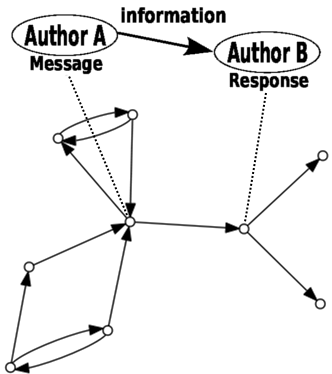
\includegraphics[width=0.5\textwidth]{figs/criaRede3_}
\caption{The formation of interaction networks from exchanged messages. Each vertex represents a participant. A reply message from author B to a message from author A is regarded as evidence that B received information from A and yields a directed edge. Multiple messages add ``weight'' to a directed edge. Further details are given in Section~\ref{intNet}.}
\label{formationNetwork}
\begin{flushleft}\footnotesize
Source: By the author.\
\end{flushleft}
\end{figure}

%Edges can be created from all antecedent message authors on the message-response thread to each message author.
%We only linked the immediate antecedent to the new message author, both for simplicity and because in adding two edges, $x\rightarrow y$ and $y\rightarrow z$, there is also a weaker connection between $x$ and $z$. Potential interpretations for this weaker connection are: double length, half weight or with one more ``obstacles''. This suggests the adequacy of centrality measurements to account for the connectivity of a node with all other nodes, such as betweenness centrality, eigenvector centrality and accessibility~\cite{luMeasures,access}.

\subsection{Topological metrics}\label{measures}

The topology of the networks was characterized 
by a small selection of the most basic 
and fundamental measurements for each vertex~\cite{newmanBook},
as introduced in Section~\ref{se:intMea}.
The betweenness centrality index was computed for weighted digraphs as specified in~\cite{faster}.

The non-standard metrics below were formulated to capture symmetries in the activity of participants:

\begin{itemize}
\item Asymmetry of vertex $i$: $asy_i=\frac{k_i^{in}-k_i^{out}}{k_i}$.
\item Average asymmetry of edges at vertex $i$:\\ $\mu_i^{asy}=\frac{\sum_{j\in J_i} e_{ji}-e_{ij}}{|J_i|}$, where $e_{ij}$ is 1 if there is an edge from $i$ to $j$, and $0$ otherwise, and $J_i$ is the set of neighbors of vertex $i$.
\item Standard deviation of asymmetry of edges:\\ $\sigma_i^{asy}=\sqrt{\frac{\sum_{j\in J_i}[\mu^{asy}_i -(e_{ji}-e_{ij}) ]^2 }{|J_i|} }$.
\item Disequilibrium: $dis_i=\frac{s_i^{in}-s_i^{out}}{s_i}$.
\item Average disequilibrium of edges:\\ $\mu_i^{dis}=\frac{\sum_{j \in J_i}\frac{w_{ji}-w_{ij}}{w_{ji}+w_{ij}}}{|J_i|}$, where $w_{xy}$ is the weight of edge $x\rightarrow y$ and zero if there is no such edge.
\item Standard deviation of disequilibrium of edges: $\sigma_i^{dis}=\sqrt{\frac{\sum_{j\in J_i}\left[\mu^{dis}_i-\frac{w_{ji}-w_{ij}}{w_{ji}+w_{ij}}\right]^2}{|J_i|}}$.
\end{itemize}

Standard metrics are used for the Erd\"os sectioning (described in the next section).
Both standard and non-standard metrics are used
for performing principal component analysis (PCA) (as described in Section~\ref{sec:pca}).


\subsection{Erd\"os sectioning}\label{sectioning}
It is often useful to think of vertices as hubs, peripheral and intermediary. We have therefore derived the peripheral, intermediary and hub sectors of an empirical network from the comparison against an Erd\"os-R\'enyi network with the same number of edges and vertices,
as depicted in Figure~\ref{fig:setores}. We refer to this procedure as \emph{Erd\"os sectioning}, with the resulting sectors being named as \emph{Erd\"os sectors}. The Erd\"os sectioning was recognized as a theoretical possibility by M. O. Jackson in his video lectures~\cite{3setores}, but to our knowledge it has not as yet been applied to empirical data.

The degree distribution $\widetilde{P}(k)$ of a real network with a scale-free profile $\mathcal{N}_f(N,z)$ with $N$ vertices and $z$ edges has less
average degree nodes than the distribution $P(k)$ of an Erd\"os-R\'enyi
network with the same number of vertices and edges. Indeed, we define in this work the intermediary sector of a network to be the set of all the nodes whose degree is less abundant in the real network than on the Erd\"os-R\'enyi model:

\begin{equation}\label{criterio}
\widetilde{P}(k)<P(k) \Rightarrow \text{k is intermediary degree}
\end{equation}

If $\mathcal{N}_f(N,z)$ is directed and has no self-loops, the probability of the existence
of an edge between two arbitrary vertices is $p_e=\frac{z}{N(N-1)}$.
A vertex in the ideal Erd\"os-R\'enyi digraph with the same number of vertices and edges, and thus the same probability $p_e$ for the presence of an edge, will have degree $k$ with probability

\begin{equation}
P(k)=\binom{2(N-1)}{k}p_e^k(1-p_e)^{2(N-1)-k}
\end{equation}

The lower degree fat tail corresponds to the border vertices, i.e. the peripheral sector or periphery where $\widetilde{P}(k)>P(k)$ and $k$ is lower than any value of $k$ in the intermediary sector.
The higher degree fat tail is the hubs sector, i.e. $\widetilde{P}(k)>P(k)$ and $k$ is higher than any value of $k$ in the intermediary sector. The reasoning for this classification is as follows: vertices so connected that they are virtually nonexistent in the Erd\"os-R\'enyi model, are coherently associated to the hubs sector.
Vertices with very few connections, which are way more abundant than expected in the Erd\"os-R\'enyi model,
are assigned to the periphery.
Vertices with degree values predicted as the most abundant in the Erd\"os-R\'enyi model,
near the average, and less frequent in the real network, are classified as intermediary.

\clearpage
\begin{figure}[!h]
\centering
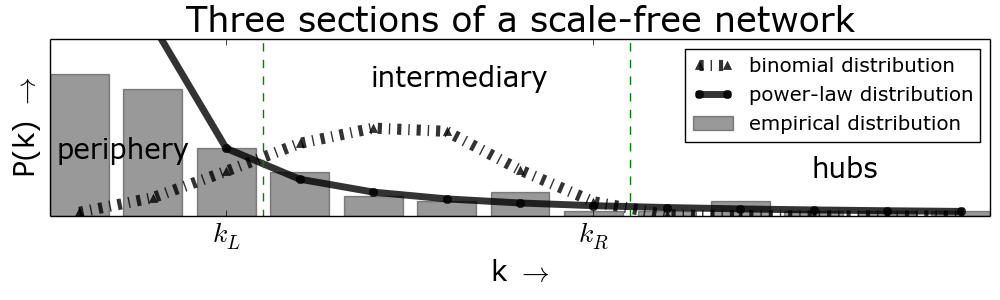
\includegraphics[width=\textwidth]{figs/fser__}
\caption{Classification of vertices by comparing degree
distributions~\cite{3setores}.
The binomial distribution of the Erd\"os-R\'enyi network model exhibits more intermediary vertices, while a scale-free network, associated with the power-law distribution, has more peripheral and hub vertices. The sector borders are defined with respect to the intersections of the distributions. Characteristic degrees are in the compact intervals: $[0,k_L]$, $(k_L,k_R]$, $(k_R,k_{max}]$ for the periphery, intermediary and hub sectors, the ``Erd\"os sectors''.
The connectivity distribution of empirical interaction networks, e.g. derived from email lists, can be sectioned by comparison against the associated binomial distribution with the same number of vertices and edges. In this figure, a snapshot of 1000 messages from CPP list yields the degree distribution of an interaction network of 98 nodes and 235 edges. A thorough explanation of the method is provided in Section~\ref{sectioning}.}
\label{fig:setores}
\begin{flushleft}\footnotesize
Source: By the author.\
\end{flushleft}
\end{figure}

To ensure statistical validity of the histograms, bins can be chosen to contain at least $\eta$ vertices of the real network.
The range $\Delta$ of incident values of degree $k$ should be partitioned in $m$ parts $\Delta=\cup_{i=1}^m \Delta_i$,
with $\Delta_i\cap \Delta_j=\emptyset \; \forall\; i \neq j$ and:
%\begin{equation}
%\begin{split}
\begin{align}
\Delta_i =\Biggl\{ k\;\; & | & \overline{\Delta}_{i-1}< &\, k\leq l \text{ and }\;\;\;\;\;\;\;\;\;\;\;\;\nonumber\\
& \Biggl[ \Bigl[ & N - \sum_{k=0}^{\overline{\Delta}_{i-1}} & \eta_k< \eta \text{ and } l = \overline{\Delta} \Bigr] \text{ or }\\
& \Bigl[ & \sum_{k=\overline{\Delta}_{i-1}+1}^l & \eta_k \geq \eta \text{ and }\;\;\;\;\;\;\nonumber\\
& \Bigl( &\sum_{k=\overline{\Delta}_{i-1}+1}^{l-1} & \eta_k < \eta \text{ or } l=\overline{\Delta}_{i-1}+1 \Bigr) \;\Bigr] \Biggr] \Biggr\}\nonumber
\end{align}
%\end{split}
%\end{equation}

\noindent where $\eta_k$ is the number of vertices with degree $k$,
while $\overline{\Delta}_{(i)}=max(\Delta_{(i)})$, and $\overline{\Delta}_{0}=-1$.
% and $\overline{\Delta}_{i}<l\leq max(\Delta)$.
Equation~\ref{criterio} can now be written in the form:

\begin{equation}\label{criterio2}
\begin{split}
\sum_{x=min(\Delta_i)}^{\overline{\Delta}_i} \widetilde{P}(x) < \sum_{x=min(\Delta_i)}^{\overline{\Delta}_i} P(x) \Leftrightarrow \\
\Leftrightarrow \Delta_i \text{ spans intermediary degree values.}
\end{split}
\end{equation}

If the strength $s$ is used for comparison of the real network against the Erd\"os-R\'enyi model,
$P$ remains the same, but $P(\kappa_i)$ with $\kappa_i=\frac{s_i}{\overline{w}}$ should be used, where $\overline{w}=\frac{\sum_is_i}{2z}$ is the average weight of an edge and $s_i$ is the strength of vertex $i$. For in and out degrees ($k^{in}$, $k^{out}$), the real network should be compared against
\begin{equation}
\hat{P}(k^{way})=\binom{N-1}{k^{way}}p_e^k(1-p_e)^{N-1-k^{way}},
\end{equation}

\noindent where \emph{way} can be \emph{in} or \emph{out}. In and out strengths ($s^{in}$, $s^{out}$) are divided by $\overline{w}$ and compared also using $\hat{P}$. Note that $p_e$ remains the same, as each edge yields an incoming (or outgoing) edge, and there are at most $N(N-1)$ incoming (or outgoing) edges, thus $p_e=\frac{z}{N(N-1)}$, as with the total degree.

In other words, let $\gamma$ and $\phi$ be integers in the intervals $1 \leq \gamma \leq 6$, $1 \leq \phi \leq 3$, and each of the basic six Erd\"os sectioning possibilities $\{E_{\gamma}\}$ have three Erd\"os sectors $E_{\gamma}= \{e_{\gamma, \phi} \}$ defined as

\begin{alignat}{3}\label{eq:part}
e_{\gamma,1}&=\{\;i\;|\;\overline{k}_{\gamma,L}\geq&&\overline{k}_{\gamma,i}\} \nonumber \\
e_{\gamma,2}&=\{\;i\;|\;\overline{k}_{\gamma,L}<\;&&\overline{k}_{\gamma,i}\leq\overline{k}_{\gamma,R}\} \\ 
e_{\gamma,3}&=\{\;i\;|\;&&\overline{k}_{\gamma,i}>\overline{k}_{\gamma,R}\} \nonumber,
\end{alignat}

\noindent where $\{\overline{k}_{\gamma,i}\}$ is

\begin{equation}
\begin{split}
\overline{k}_{1,i}&=k_i \\
\overline{k}_{2,i}&=k_i^{in} \\
\overline{k}_{3,i}&=k_i^{out} \\
\overline{k}_{4,i}&=\frac{s_i}{\overline{w}} \\
\overline{k}_{5,i}&=\frac{s_i^{in}}{\overline{w}} \\
\overline{k}_{6,i}&=\frac{s_i^{out}}{\overline{w}}
\end{split}
\end{equation}

\noindent and both $\overline{k}_{\gamma,L}$ and $\overline{k}_{\gamma,R}$ are found using $P(\overline{k})$ or $\hat{P}(\overline{k})$ as described above and illustrated in Figure~\ref{fig:setores}.

Since different metrics can be used to identify the three types of vertices, more than one metric can be used simultaneously, which is convenient when analysing small networks,
such as the cases where only 50 messages are considered in the supporting information document of~\cite{stab}.
%For example, a very stringent criterion can be used, according to which a vertex is only regarded as pertaining to a sector if it is so for all the metrics.
After a careful consideration of possible combinations, these were reduced to six:

\begin{itemize}
\item Exclusivist criterion $C_1$: vertices are only classified if the class is the same according to all metrics. In this case, vertices classified do not usually reach $N$ (or 100\%).

\item Inclusivist criterion $C_2$: a vertex has the class given by any of the metrics. Therefore, a vertex may belong to more than one class, and the total number of memberships may exceed $N$ (or 100\%).

\item Exclusivist cascade $C_3$: vertices are only classified as hubs if they are hubs according to all metrics. Intermediary are the vertices classified either as intermediary or hubs with respect to all metrics. The remaining vertices are regarded as peripheral.

\item Inclusivist cascade $C_4$: vertices are hubs if they are classified as such according to any of the metrics. The remaining vertices are intermediary if they belong to this category for any of the metrics. Peripheral vertices are those which are classified as such with respect to all metrics.

\item Exclusivist externals $C_5$: vertices are hubs if they are classified as such according to all the metrics. Vertices are peripheral if they are peripheral or hubs for all metrics. The remaining nodes are intermediary.

\item Inclusivist externals $C_6$: hubs are vertices classified as hubs according to any metric. The remaining vertices are peripheral if they are classified as such according to any metric. The rest of the vertices are intermediary.
\end{itemize}

Using Equations~(\ref{eq:part}), these \emph{compound criteria} $C_\delta$, with $\delta$ integer in the interval $1\leq\delta\leq6$, can be specified as:

%\begin{alignat}{3}
\begin{equation}
\begin{split}
%\begin{multline}
C_1&=\{c_{1,\phi}=\left\{i\mid i\;\in e_{\gamma,\phi}, \;\forall\; \gamma\}\right\} \\
C_2&=\{c_{2,\phi}=\left\{i\mid \exists \;\;\gamma: i \in e_{\gamma,\phi}\}\right\} \\
C_3&=\{c_{3,\phi}=\left\{i\mid i\;\in e_{\gamma,\phi'}, \;\forall\; \gamma,\;\forall\;\phi'\geq \phi\}\right\} \\
C_4&=\{c_{4,\phi}=\left\{i\mid i\;\in e_{\gamma,\phi'}, \;\forall\; \gamma,\;\forall\;\phi'\leq \phi\}\right\} \\
C_5&=\{c_{5,\phi}=\left\{i\mid i\;\in e_{\gamma,\phi'}, \;\forall\; \gamma,\right.\\
&\;\;\;\;\;\;\;\;\;\;\;\;\;\;\;\;\;\; \left.\;\forall\;(\phi'+1)\%4\leq (\phi+1)\%4\}\right\} \\
C_6&=\{c_{6,\phi}=\left\{i\mid i\;\in e_{\gamma,\phi'}, \;\forall\; \gamma,\right.\\
&\;\;\;\;\;\;\;\;\;\;\;\;\;\;\;\;\;\; \left.\;\forall\;(\phi'+1)\%4\geq (\phi+1)\%4\}\right\} \\
%\end{multline}
\end{split}
\end{equation}
%\end{alignat}

Notice that the exclusivist cascade is the same sectioning of an inclusivist cascade from periphery to hubs, but with inverted order of sectors. 
The simplification of all possible compound possibilities to the small set listed above might be formalized in strict mathematical terms, but this was considered out of the scope for current interests.
%\subsubsection{Sectioning of networks in peripheral, intermediary and hubs sectors}\label{sectioning}


\subsection{Principal Component Analysis of topological metrics}\label{sec:pca}
Principal Component Analysis (PCA) is a well documented technique~\cite{pca} and is used here to address the following questions: 1) which metrics contribute to each principal component and in what proportion; 2) how much of the dispersion is concentrated in each component; 3) which are the expected values and dispersions for these quantities over various networks. This enables one to characterize human interaction networks in terms of the relative importance of network metrics and the way they combine.

Let $\mathbf{X}=\{X[i,j]\}$ be a matrix where each element is the value
of the metric $j$ at vertex $i$.
Let
$\mu_X [j]=\frac{\sum_i X[i,j]}{I}$ be the mean of metric $j$ over all $I$ vertices, 
$\sigma_X [j]=\sqrt{\frac{\sum_i (X[i,j]-\mu_X [j])^2}{I}}$ the standard deviation of metric $j$,
and $\mathbf{X'}=\{X'[i,j]\}=\left\{\frac{X[i,j]-\mu_X[j]}{\sigma_X[j]}\right\}$ 
the matrix with the \emph{z-score} of each metric. 
Let $\mathbf{V}=\{V[j,k]\}$ be the matrix $J\times J$ of eigenvectors
of the covariance matrix $\mathbf{C}$
of $\mathbf{X'}$, one eigenvector per column.
Each eigenvector combines the original metrics into one principal component, therefore
$V'[j,k]=100\frac{|V[j,k]|}{\sum_{j'} |V[j',k]|}$
is the percentage of the principal component $k$
that is proportional to the metric $j$.
%With $k$ eigenvectors 
%$D[k]$,
%it is enough to 
Let $\mathbf{D}=\{D[k]\}$ be the eigenvalues associated with the eigenvectors $\mathbf{V}$,
then $D'[k]=100\frac{D[k]}{\sum_{k'}D[k']}$
is the percentage of total dispersion of the system that the principal component $k$
is responsible for.
We consider, in general, the three largest eigenvalues and
the respective eigenvectors in percentages:
$\{(D'[k],\;V'[j,k])\}$.
These usually sum up between 60 and 95\% of the dispersion
and reveal patterns for a first analysis.
In particular, 
given $L$ snapshots $l$ of the interaction network,
we are interested in the mean
$\mu_{V'}[j,k]$
and the standard deviation $\sigma_{V'}[j,k]$ 
of the contribution of metric $j$ to the principal component $k$,
and the mean
$\mu_{D'}[k]$
and the standard deviation 
$\sigma_{D'}[k]$
of the contribution of the component $k$ to the dispersion
of the system:

\begin{align}\label{eq:pca}
\mu_{V'}[j,k] &=\frac{\sum_{l=1}^L V'[j,k,l]}{L}\nonumber\\
\sigma_{V'}[j,k]&=\sqrt{\frac{\sum_{l=1}^L (\mu_{V'}-V'[j,k,l])^2}{L}}\\\nonumber
\mu_{D'}[k]&=\frac{\sum_{l=1}^L D'[k,l]}{L}\\\nonumber
\sigma_{D'}[k]&=\sqrt{\frac{\sum_{l=1}^L (\mu_{D'}-D'[k,l])^2}{L}}
\end{align}

The covariance matrix 
$\mathbf{C}$ is the correlation matrix because $\mathbf{X'}$ is normalized.
Therefore, $\mathbf{C}$ is also directly observed as a first clue for patterns
by the most simple associations:
low absolute values indicate low correlation (and a possible independence);
high values indicate positive correlation;
negative values with a high absolute value indicate negative correlation.
Notice that in this case the variable $k$ is not the degree value
but a principal component.
In the results, the principal components are numbered
according to the magnitude of associated eigenvalue and $k$ is incorporated into
the notation (e.g. PC2 for metrics of $\mu_{V'}[j,2]$).


\subsection{Evolution of the networks}\label{sec:viz}
The evolution of the networks was observed within 
sequences of snapshots. In each sequence, a fixed number of messages,
i.e. the window size $ws$, was used for all snapshots.
%was considered with different shifts in the message timeline to obtain snapshots.
The snapshots were made disjoint in the message timeline, and were used to perform both PCA with topological metrics and Erd\"os sectioning. 
Figures and tables were usually inspected with 
$ws=\{50, 100, 200, 400, 500, 800, 1000, 2000, 2500, 5000, 10000\}$ messages. Variations in the number of vertices, edges
and other network characteristics, within the same window size $ws$,
are given in the supporting information document of~\cite{stab}. 

\subsection{The Versinus graph visualization method}\label{sec:versinus0}
Network structures were mapped to video animations, sound and musical structures developed for this research~\cite{animacoes}.% ,galGmane,appGmane}.
Such \emph{audiovisualizations} were crucial in the initial steps and
to guide the research into the most important features of network evolution.
Versinus is a visualization method for dynamic graphs based on experimental observations.
This method received dedicated attention by recurrence of the suggestion, by fellow researchers,
to write about it. 
In visualizing a network, the method consists of creating an animation
of a fixed-size message sliding window (e.g. 400 messages) and 
partitioning the network in two fixed-layout segments:
a sinusoid period for the most connected vertices (hubs and intermediary)
and a straight line for the less connected (peripheral).
A vertex holds the same position throughout the animation. Also,
visual cues of properties - such as color, height and width,
and rank of vertex with degree criteria - play a central role.
Numbers with individual measurements for each vertex blink periodically.
Versinus differs from the few works on the visualization of dynamic
graphs because it is a simple method developed for practical needs and is the result of experimentations,
although a number of criteria have guided its development~\cite{Viz1,eades,Viz3}.

Let $\Delta$ be a fixed number of messages (e.g. $\Delta=400$).
Let also $s_{i}^{i+\Delta}$ be sets of $\Delta$ consecutive email messages along time.
A sequence $S^{\Delta,M}$ of such sets,
with the first message positioned in each the $M$ messages (e.g. $M=20000$),
can be written as: 

\begin{equation}
S^{\Delta,M}=\{s_i^{i+\Delta}\}_{i=0}^{M-\Delta}
\end{equation}

Each set $s_i$ yields an interaction network, as described in Section~\ref{intNet}.
Each of such sequence $S^{\Delta,M}$ of sets presents stable properties,
while each participant exhibits a wide variation of characteristics.
Understanding the mechanisms of this compatibility (unstable vertices and stable network)
led to experimenting with a series of layouts and visualization techniques, from which Versinus emerged.

Taking advantage from the fact that vertices are roughly split into usual $80\%$ of peripheral, $15\%$ of intermediary and $5\%$ of hubs (see results in the next Chapter),
hubs are laid on the first half of a sinusoid,
intermediary on the second half,
and peripheral on the straight line.
This configuration can be improved in various forms, to which Section~\ref{sec:verref} is dedicated.
Figure~\ref{fig:versinus} has an image of such a layout.
The fixed position of each vertex is defined by the overall structure,
i.e. with respect to all $M$ messages.

\begin{figure}[h!]
\begin{center}
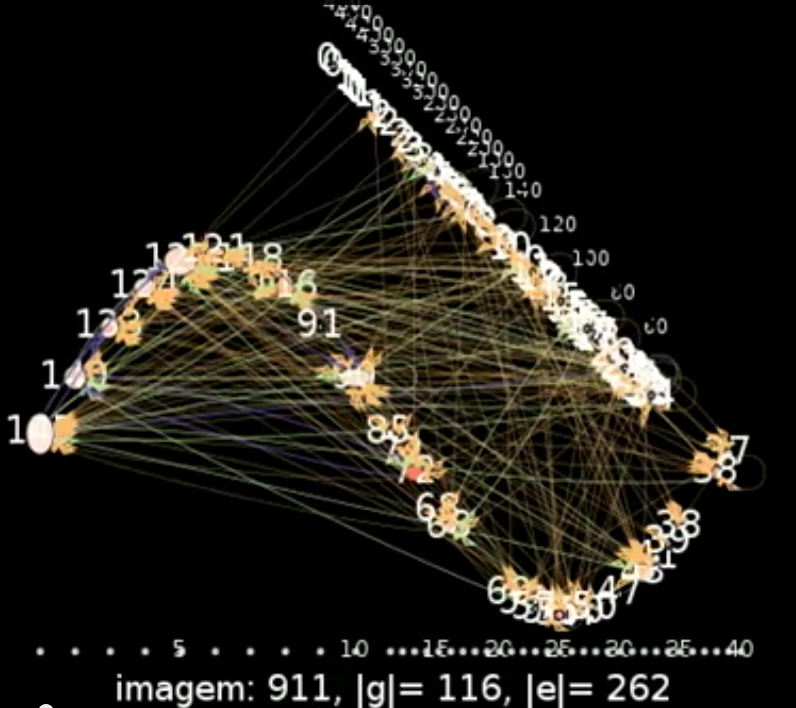
\includegraphics[scale=.45]{figs/versinus_}
\caption{The Versinus visualization method in use. 5\% of the most connected vertices (hubs) are on the left half-period of the sinusoid.
15\% of the most connected remaining vertices are on the right half-period.
80\% of the least connected vertices are on the straight line, above the sinusoidal shape.
White dots in the bottom with numbers keep track of node position in the overall degree ordering.
Measurements blink periodically near the vertices they are related to.}
\label{fig:versinus}
\begin{flushleft}\footnotesize
Source: By the author.\
\end{flushleft}
\end{center}
\end{figure}


\subsection{Textual metrics}
This work focuses on very simple metrics derived from texts as they have been sufficient for current interests.
Such metrics are:
\begin{itemize}
\item Frequency of characters: letters, vowels, punctuations and uppercase letters.
\item Number of tokens, frequency of punctuations among tokens, frequency of known words, frequency of words that have Wordnet synsets, frequency of tokens that are stopwords.
\item Mean and standard deviation for word, token sentence and message sizes.
\item Fraction of morphosyntactic classes, such as adverbs, adjectives, nouns and other POS (Part-Of-Speech) tags.
	We implemented a Brill POS tagger because of the massive amount of textual data that we had to analyze (the Brill tagger is very fast).
	We used the ``universal'' tagset described in~\cite{petrov} (developed to account for many languages) and trained the tagger with both Brown and Treebank corpus\footnote{We
		used the full Brown corpus while only 5\% of the Penn Treebank (as included in NLTK~\cite{trabNLTK}).}
	divided into 80/20\% of sentences for training and evaluation. The tagger achieved $94.95\%$ of accuracy.
\item Fraction of words in each Wordnet~\cite{wordnet} top-most hypernyms,
such as abstraction and physical entities for nouns or act for verbs.
\item Mean and standard deviation of the number of Wordnet synset relations, such as holonyms and meronyms, domains, lemmas and verb groups.
\end{itemize}
% \noindent To such metrics are dedicated Tables~\ref{tab:cha},~\ref{tab:tokens},~\ref{tab:sizesTokens},~\ref{tab:sizesSents},~\ref{tab:sizesMsgs},~\ref{tab:pos}.

This choice is based on: 1) the lack of such information in the literature, to the best of our knowledge; 
2) potential relations of these incidences with topological aspects, such as connectivity;
3) the interdependence of textual artifacts suggests that simple metrics should reflect complex and more subtle aspects.
A preliminary study, with the complete works from the Brazilian writer Machado de Assis~\cite{machado},
made clear that these metrics vary with respect to style.

\subsubsection{About Wordnet}
In this thesis, we made use of the statistics derived from the incidence of Wordnet synsets and their characteristics.
This calls for a brief description of what Wordnet is, what is a synset and what are such characteristics:
\begin{itemize}
\item Wordnet: a lexical database for the English language released in a BSD style license. It groups synonyms into synsets, provides a number of relations among the synsets, definitions and use examples.
\item Synset: defined by Wordnet documentation as a set of one or more synonyms that are (somewhat) interchangeable without changing the true value of the proposition in which they occur.
\item Synset characteristics: a synset is associated to other synsets by a number of semantic relations which differ with the POS tag attributed to them.
Examples of such relations include hyponyms and hypernyms (respectively less and more general terms), meronyms and holonyms (respectively is part of and has part), lemmas (canonical forms of a word), similar words by semantic criteria, entailments.
Some characteristics are derived from the synset in relation to the whole Wordnet network.
In this respect, we used only the maximum and minimum depth of the synset, which are respectively the maximum and minimum number of hypernyms from the synset to the root synset (e.g. 'thing' for nouns).
\end{itemize}

\subsubsection{Relating text and topology}\label{sec:ks}
The topological and textual metrics were related by:
\begin{enumerate}
\item textual metrics in hub, intermediary and peripheral network sectors, which are delimited by topological criteria as described in Section~\ref{sectioning}.
\item Correlation of metrics of each vertex, facilitating pattern detection involving topology of interaction and language.
\item Principal components formation derived from the usual Principal Component Analysis.
\end{enumerate}

An adaptation of the Kolmogorov-Smirnov test was used to observe differences in textual content, as follows.
Let $F_{1,n}$ and $F_{2,n'}$ be two empirical distribution functions, where $n$ and $n'$ are the number of observations on each sample.
The two-sample Kolmogorov-Smirnov test rejects the null hypothesis (that the samples are drawn from the same underlying distribution) if:
\begin{equation}\label{eq:ks}
D_{n,n'} > c(\alpha)\sqrt{\frac{n+n'}{nn'}}
\end{equation}

\noindent where $D_{n,n'}=sup_x[F_{1,n}-F_{2,n'}]$ is the Kolmogorov-Smirnov statistic
and $c(\alpha)$ is related to the significance level $\alpha$ by:

\begin{table}[H]
\centering
\begin{tabular}{l||c|c|c|c|c|c}\hline
$\alpha$ & 0.1 & 0.05 & 0.025 & 0.01 & 0.005 & 0.001 \\
$c(\alpha)$ & 1.22 & 1.36 & 1.48 & 1.63 & 1.73 & 1.95 \\\hline
\end{tabular}
\begin{flushleft}\footnotesize
	Source: KOLMOGOROV-SMIRNOV test~\cite{wpksTest}.\
\end{flushleft}
\end{table}

We need to compare empirical distribution functions,
therefore $D_{n,n'}$ is given, as are $n$ and $n'$.
All terms in equation~\ref{eq:ks} are positive and $c(\alpha)$ can be isolated:

\begin{equation}\label{eq:ks2}
c(\alpha) < \frac{D_{n,n'}}{\sqrt{\frac{n+n'}{nn'}}} = c'
\end{equation}

When $c'$ is high, corresponding low values of $\alpha$ favor rejecting the null hypothesis.
For example, when $c'$ is greater than $\approx 1.7$, one might assume that $F_{1,n}$ and $F_{2,n'}$ differ.
We used $c'$ as a measure of how much
the distributions differ
and for deriving hypotheses
about how different are the underlying mechanisms of generation of texts.
We made systematic measurements of the $c'$ statistic in~\cite{kolmSmir}
which illustrate that $c'$ and $D_{n,n'}$ are useful in considering the
similarity or difference in the distributions underlying sets of observations.
A note of caution should be given here: what is a difference in distributions
might vary with context.
A $D_{n,n'}$ of only $0.0001$ will yield a very large $c'$ if $n$ and $n'$ are large enough.
On the other hand, a large $D_{n,n'}$ with a small $c'$ is not a strong evidence that
the distributions differ.
Therefore, we consider both $D_{n,n'}$ and $c'$ simultaneously in our analysis.

% ---
% Capítulo 3
% ---
\chapter{Results and Discussion}
\label{ch:disc}
% Será necessária Introdução
% ao Capítulo e talvez divisão em tópicos?

Two main types of results will be discussed in this Chapter. In the first, we analyze the stability in the topology of networks derived from email lists, also including networks from Twitter, Facebook and ParticipaBR (a Brazilian federal social participation portal) in order to confirm the results. In the second type, we analyze the distinct language usage of the different classes of participants in the email lists networks.
We also describe results obtained in the visualization of dynamic networks
and from an assembling of data from diverse provenance into linked data, which were essential for supporting the research that led to the two types of results mentioned.


\subsection{Activity along time}\label{constDisc}
Regular patterns of activity in email lists were observed along time
in the scales of seconds, minutes, hours, days and months.
Histograms in each of the time scales were computed as were circular average and dispersion values, and the results are given in Tables~\ref{tab:circ}-\ref{tab:min22}. For example, uniform activity is found with respect to seconds, minutes and days of the months. Weekend days exhibit about half the activity of regular weekdays, and there is a peak of activity between 11am and noon.


\begin{table}
\caption{The rescaled circular mean $\theta_\mu'$ and the circular dispersion $\delta(z)$, described in Section~\ref{sec:mtime}, for different timescales. This example table was constructed using all LAD messages, and the results are the same for other lists, as shown in the Supporting Information document of~\cite{stab}. The most uniform distribution of activity was found in seconds and minutes. Hours of the day exhibited the most concentrated activity (lowest $\delta(z)$), with mean between 2 p.m. and 3 p.m. ($\theta'=-9.61$). Weekdays, days of the month and months have mean near zero (i.e. near the beginning of the week, month and year) and high dispersion. Note that $\theta_u'$ has the dimensional unit of the corresponding time period while $\delta(z)$ is dimensionless.}
\begin{center}
\begin{tabular}{ l|| c|c }
\hline
%scale & $\theta_\mu'$ & $S(z)$ & $Var(z)$ & $\delta(z)$ & $\frac{max(incidence)}{min(incidence)}$ & $ \mu_{\frac{max(incidence')}{min(incidence')}} $ & $ \sigma_{\frac{max(incidence')}{min(incidence')} } $ \\ \hline\hline
%& $\theta_\mu'$ & $S(z)$ & $Var(z)$ & $\delta(z)$  \\ \hline\hline
scale & mean $\theta_\mu'$ & dispersion $\delta(z)$  \\ \hline
seconds    & --//--  & 9070.17     \\\hline
minutes    & --//--  & 205489.40   \\\hline
hours      & -9.61   & 4.36        \\\hline
weekdays   & -0.03   & 29.28       \\\hline
month days & -2.65   & 2657.77     \\\hline
months     & -0.56   & 44.00       \\\hline

\end{tabular}
\begin{flushleft}\footnotesize
Source: By the author.\
\end{flushleft}
\end{center}
\label{tab:circ}
\end{table}

\begin{table}
\caption{Activity percentages along the hours of the day. Nearly identical distributions were observed on other social systems as shown in the Supporting Information document of~\cite{stab}.
Highest activity was observed between noon and 6pm (with 1/3 of total day activity), followed by the time period between 6pm and midnight.
Around 2/3 of the activity takes place from noon to midnight
but the activity peak occurs between 11 a.m. and 12 p.m.
This table shows results for the activity in CPP.}
\footnotesize
\begin{center} 
 \begin{tabular}{ l || c | c | c | c | c | c }\hline
  & 1h & 2h & 3h & 4h & 6h & 12h \\\hline \hline
 0h  &  \multirow{1}{*}{ 3.66 }   &  \multirow{2}{*}{ 6.42 }   &  \multirow{3}{*}{ 8.20 }   &  \multirow{4}{*}{ 9.30 }   &  \multirow{6}{*}{ 10.67 }   &  \multirow{12}{*}{ 33.76 }  \\\cline{2-2} 
 1h  &  \multirow{1}{*}{ 2.76 }   &   &   &   &   &  \\\cline{2-2}\cline{3-3} 
 2h  &  \multirow{1}{*}{ 1.79 }   &  \multirow{2}{*}{ 2.88 }   &   &   &   &  \\\cline{2-2}\cline{4-4} 
 3h  &  \multirow{1}{*}{ 1.10 }   &   &  \multirow{3}{*}{ 2.47 }   &   &   &  \\\cline{2-2}\cline{3-3}\cline{5-5} 
 4h  &  \multirow{1}{*}{ 0.68 }   &  \multirow{2}{*}{ 1.37 }   &   &  \multirow{4}{*}{ 3.44 }   &   &  \\\cline{2-2} 
 5h  &  \multirow{1}{*}{ 0.69 }   &   &   &   &   &  \\\cline{2-2}\cline{3-3}\cline{4-4}\cline{6-6} 
 6h  &  \multirow{1}{*}{ 0.83 }   &  \multirow{2}{*}{ 2.07 }   &  \multirow{3}{*}{ 4.35 }   &   &  \multirow{6}{*}{ 23.09 }   &  \\\cline{2-2} 
 7h  &  \multirow{1}{*}{ 1.24 }   &   &   &   &   &  \\\cline{2-2}\cline{3-3}\cline{5-5} 
 8h  &  \multirow{1}{*}{ 2.28 }   &  \multirow{2}{*}{ 6.80 }   &   &  \multirow{4}{*}{ 21.03 }   &   &  \\\cline{2-2}\cline{4-4} 
 9h  &  \multirow{1}{*}{ 4.52 }   &   &  \multirow{3}{*}{ 18.75 }   &   &   &  \\\cline{2-2}\cline{3-3} 
 10h  &  \multirow{1}{*}{ 6.62 }   &  \multirow{2}{*}{ \textbf{ 14.23 } }   &   &   &   &  \\\cline{2-2} 
 11h  &  \multirow{1}{*}{ \textbf{ 7.61 } }   &   &   &   &   &  \\\cline{2-2}\cline{3-3}\cline{4-4}\cline{5-5}\cline{6-6}\cline{7-7} 
 12h  &  \multirow{1}{*}{ 6.44 }   &  \multirow{2}{*}{ 12.48 }   &  \multirow{3}{*}{ \textbf{ 18.95 } }   &  \multirow{4}{*}{ \textbf{ 25.05 } }   &  \multirow{6}{*}{ \textbf{ 37.63 } }   &  \multirow{12}{*}{ \textbf{ 66.24 } }  \\\cline{2-2} 
 13h  &  \multirow{1}{*}{ 6.04 }   &   &   &   &   &  \\\cline{2-2}\cline{3-3} 
 14h  &  \multirow{1}{*}{ 6.47 }   &  \multirow{2}{*}{ 12.57 }   &   &   &   &  \\\cline{2-2}\cline{4-4} 
 15h  &  \multirow{1}{*}{ 6.10 }   &   &  \multirow{3}{*}{ 18.68 }   &   &   &  \\\cline{2-2}\cline{3-3}\cline{5-5} 
 16h  &  \multirow{1}{*}{ 6.22 }   &  \multirow{2}{*}{ 12.58 }   &   &  \multirow{4}{*}{ 23.60 }   &   &  \\\cline{2-2} 
 17h  &  \multirow{1}{*}{ 6.36 }   &   &   &   &   &  \\\cline{2-2}\cline{3-3}\cline{4-4}\cline{6-6} 
 18h  &  \multirow{1}{*}{ 6.01 }   &  \multirow{2}{*}{ 11.02 }   &  \multirow{3}{*}{ 15.88 }   &   &  \multirow{6}{*}{ 28.61 }   &  \\\cline{2-2} 
 19h  &  \multirow{1}{*}{ 5.02 }   &   &   &   &   &  \\\cline{2-2}\cline{3-3}\cline{5-5} 
 20h  &  \multirow{1}{*}{ 4.85 }   &  \multirow{2}{*}{ 9.23 }   &   &  \multirow{4}{*}{ 17.59 }   &   &  \\\cline{2-2}\cline{4-4} 
 21h  &  \multirow{1}{*}{ 4.38 }   &   &  \multirow{3}{*}{ 12.73 }   &   &   &  \\\cline{2-2}\cline{3-3} 
 22h  &  \multirow{1}{*}{ 4.06 }   &  \multirow{2}{*}{ 8.36 }   &   &   &   &  \\\cline{2-2} 
 23h & \multirow{1}{*}{ 4.30 }  & & & & & \\\cline{2-2}\cline{3-3}\cline{4-4}\cline{5-5}\cline{6-6}\cline{7-7} 
 \hline\end{tabular} 
 \end{center}

\label{tab:hin}
\begin{flushleft}\footnotesize
Source: By the author.\
\end{flushleft}
\end{table}


\begin{table}
\caption{Activity percentages along weekdays.
Higher activity was observed during workweek days, with a decrease of activity on weekend days of at least one third and at most two thirds.}
\begin{center}
\begin{tabular}{ l ||  c | c | c | c | c |c | c}
\hline
& Mon & Tue & Wed & Thu & Fri & Sat & Sun  \\ \hline\hline
LAU & 15.71  & 15.81  & 15.88  & 16.43  & 15.14  & {\bf 10.13}  & {\bf 10.91} \\
LAD & 14.92  & 17.75  & 17.01  & 15.41  & 14.21  & {\bf 10.40}  & {\bf 10.31} \\
MET & 17.53  & 17.54  & 16.43  & 17.06  & 17.46  & {\bf 7.92 }  & {\bf 6.06 } \\
CPP & 17.06  & 17.43  & 17.61  & 17.13  & 16.30  & {\bf 6.81 }  & {\bf 7.67 } \\\hline

\end{tabular}
\end{center}
\label{tab:win}
\begin{flushleft}\footnotesize
Source: By the author.\
\end{flushleft}
\end{table}

In the scales of seconds and minutes, activity is uniform,
with the messages being slightly more evenly distributed in all lists than in simulations with the uniform distribution\footnote{Numpy version 1.8.2, ``random.randint'' function was used for simulations, algorithms in \url{https://github.com/ttm/percolation}.}.
In the networks, $\frac{min(incidence)}{max(incidence)} \in (0.784,.794)$ while simulations reach these values but have on average more discrepant higher and lower peaks, i.e. if $\xi=\frac{min(incidence')}{max(incidence')}$ than $\mu_\xi=0.7741 \text{ and } \sigma_\xi=0.02619$.
Therefore, the incidence of messages at each second of a minute and at each minute of an hour was considered uniform.
In these cases, the circular dispersion is maximized and the mean has little meaning as indicated in Table~\ref{tab:circ}.
As for the hours of the day, an abrupt peak is found between 11am and 12pm with the most active period being the afternoon, with one third of total daily activity, and two thirds of activity are allocated in the second 12h of each day. Days of the week revealed a decrease between one third and two thirds of activity on weekends.
Days of the month were regarded as homogeneous with an inconclusive slight tendency of the first week to be more active.
Months of the year revealed patterns matching usual work and academic calendars. The time period examined here was not sufficient for the analysis of activity along the years. These patterns are exemplified in Tables~\ref{tab:hin}-\ref{tab:min22}.


\FloatBarrier

\begin{table}
\caption{Activity along the days of the month cycle.
Nearly identical distributions are found in all systems
as indicated in the Supporting Information of~\cite{stab}. Although slightly higher activity rates are found in the beginning of the month, the most important feature seems to be the homogeneity made explicit by the high circular dispersion in Table~\ref{tab:circ}.
This specific example and empirical table correspond to the activity of the MET email list.}
\footnotesize
\begin{center}
\begin{tabular}{l || c | c | c | c}\hline
 & 1 day & 5 & 10 & 15 days \\\hline\hline
1 & \multirow{1}{*}{ 3.05 }  & \multirow{5}{*}{ 18.25 }  & \multirow{10}{*}{ 35.24 }  & \multirow{15}{*}{ 50.96 }  \\\cline{2-2}
2 & \multirow{1}{*}{ 3.38 }  & & & \\\cline{2-2}
3 & \multirow{1}{*}{ 3.62 }  & & & \\\cline{2-2}
4 & \multirow{1}{*}{ 4.25 }  & & & \\\cline{2-2}
5 & \multirow{1}{*}{ 3.94 }  & & & \\\cline{2-2}\cline{3-3}
6 & \multirow{1}{*}{ 3.73 }  & \multirow{5}{*}{ 16.98 }  & & \\\cline{2-2}
7 & \multirow{1}{*}{ 3.17 }  & & & \\\cline{2-2}
8 & \multirow{1}{*}{ 3.26 }  & & & \\\cline{2-2}
9 & \multirow{1}{*}{ 3.56 }  & & & \\\cline{2-2}
10 & \multirow{1}{*}{ 3.26 }  & & & \\\cline{2-2}\cline{3-3}\cline{4-4}
11 & \multirow{1}{*}{ 3.81 }  & \multirow{5}{*}{ 15.73 }  & \multirow{10}{*}{ 31.98 }  & \\\cline{2-2}
12 & \multirow{1}{*}{ 2.91 }  & & & \\\cline{2-2}
13 & \multirow{1}{*}{ 3.30 }  & & & \\\cline{2-2}
14 & \multirow{1}{*}{ 2.75 }  & & & \\\cline{2-2}
15 & \multirow{1}{*}{ 2.95 }  & & & \\\cline{2-2}\cline{3-3}\cline{5-5}
16 & \multirow{1}{*}{ 3.36 }  & \multirow{5}{*}{ 16.25 }  & & \multirow{15}{*}{ 49.04 }  \\\cline{2-2}
17 & \multirow{1}{*}{ 3.16 }  & & & \\\cline{2-2}
18 & \multirow{1}{*}{ 3.44 }  & & & \\\cline{2-2}
19 & \multirow{1}{*}{ 3.36 }  & & & \\\cline{2-2}
20 & \multirow{1}{*}{ 2.93 }  & & & \\\cline{2-2}\cline{3-3}\cline{4-4}
21 & \multirow{1}{*}{ 3.20 }  & \multirow{5}{*}{ 15.79 }  & \multirow{10}{*}{ 32.78 }  & \\\cline{2-2}
22 & \multirow{1}{*}{ 3.11 }  & & & \\\cline{2-2}
23 & \multirow{1}{*}{ 3.60 }  & & & \\\cline{2-2}
24 & \multirow{1}{*}{ 2.74 }  & & & \\\cline{2-2}
25 & \multirow{1}{*}{ 3.13 }  & & & \\\cline{2-2}\cline{3-3}
26 & \multirow{1}{*}{ 3.13 }  & \multirow{5}{*}{ 16.99 }  & & \\\cline{2-2}
27 & \multirow{1}{*}{ 3.07 }  & & & \\\cline{2-2}
28 & \multirow{1}{*}{ 3.61 }  & & & \\\cline{2-2}
29 & \multirow{1}{*}{ 3.60 }  & & & \\\cline{2-2}
30 & \multirow{1}{*}{ 3.57 }  & & & \\\cline{2-2}\cline{3-3}\cline{4-4}\cline{5-5}
\hline\end{tabular}
\end{center}

\label{tab:min}
\begin{flushleft}\footnotesize
Source: By the author.\
\end{flushleft}
\end{table}

\begin{table}
\caption{Activity percentages on months along the year. Activity is usually concentrated in Jun-Aug and/or in Dec-Mar, potentially due to academic calendars, vacations and end-of-year holidays. This table corresponds to activity in LAU. Similar results are shown for other lists in the Supporting Information document of~\cite{stab}.}
\footnotesize
\begin{center}
\begin{tabular}{| l || c | c | c | c | c |}\hline
 & m. & b. & t. & q. & s. \\\hline
Jan & \multirow{1}{*}{ 10.22 }  & \multirow{2}{*}{ 19.56 }  & \multirow{3}{*}{ 28.24 }  & \multirow{4}{*}{ 35.09 }  & \multirow{6}{*}{ 49.16 }  \\\cline{2-2}
Fev & \multirow{1}{*}{ 9.34 }  & & & & \\\cline{2-2}\cline{3-3}
Mar & \multirow{1}{*}{ 8.67 }  & \multirow{2}{*}{ 15.53 }  & & & \\\cline{2-2}\cline{4-4}
Apr & \multirow{1}{*}{ 6.86 }  & & \multirow{3}{*}{ 20.93 }  & & \\\cline{2-2}\cline{3-3}\cline{5-5}
Mai & \multirow{1}{*}{ 7.28 }  & \multirow{2}{*}{ 14.07 }  & & \multirow{4}{*}{ 30.36 }  & \\\cline{2-2}
Jun & \multirow{1}{*}{ 6.80 }  & & & & \\\cline{2-2}\cline{3-3}\cline{4-4}\cline{6-6}
Jul & \multirow{1}{*}{ 8.97 }  & \multirow{2}{*}{ 16.29 }  & \multirow{3}{*}{ 24.47 }  & & \multirow{6}{*}{ 50.84 }  \\\cline{2-2}
Ago & \multirow{1}{*}{ 7.32 }  & & & & \\\cline{2-2}\cline{3-3}\cline{5-5}
Set & \multirow{1}{*}{ 8.18 }  & \multirow{2}{*}{ 16.25 }  & & \multirow{4}{*}{ 34.55 }  & \\\cline{2-2}\cline{4-4}
Out & \multirow{1}{*}{ 8.06 }  & & \multirow{3}{*}{ 26.36 }  & & \\\cline{2-2}\cline{3-3}
Nov & \multirow{1}{*}{ 7.64 }  & \multirow{2}{*}{ 18.30 }  & & & \\\cline{2-2}
Dez & \multirow{1}{*}{ 10.66 }  & & & & \\\cline{2-2}\cline{3-3}\cline{4-4}\cline{5-5}\cline{6-6}
\hline\end{tabular}
\end{center}
\label{tab:min22}
\begin{flushleft}\footnotesize
Source: By the author.\
\end{flushleft}
\end{table}


\subsection{Stable sizes of Erd\"os sectors}\label{subsec:pih}

The distribution of vertices in the hub, intermediary and periphery Erd\"os sectors is remarkably stable along time if the snapshots hold 200 or more messages,
as it is clear in Figure~\ref{fig:sectIL} and in the figures of the Supporting Information document of~\cite{stab}.
%Moreover, all email lists analyzed exhibit the same distribution profile.
Activity is highly concentrated on the hubs, while a very large number of peripheral vertices contribute to only a fraction of the activity.
This is expected for a system with a scale-free profile, as confirmed with the distribution of activity among participants in Table~\ref{autores}.

Typically, $[3\%-12\%]$ of the vertices are hubs,
$[15\%-45\%]$ are intermediary and $[44\%-81\%]$ are peripheral,
which is consistent with other studies~\cite{secFree}.
These results hold for the total, in and out degrees and strengths.
Stable sizes are also observed for 100 or less messages if the classification 
of the three sectors is performed with one of the compound criteria established in Section~\ref{sectioning}. The networks often hold this basic structure with as few as 10-50 messages, i.e. concentration of activity and the abundance of low-activity participants take place even with very few messages, which is highlighted in the Supporting Information document of~\cite{stab}.
A minimum window size for the observation of more general properties might be inferred by monitoring 
both the giant component and the degeneration of the Erd\"os sectors.

In order to support the generality of these findings,
we list the Erd\"os sector sizes of 12 networks from Facebook, Twitter and Participabr in the final tables of the
Supporting Information document of~\cite{stab}.
The fractions of hubs, intermediary and peripheral nodes are
essentially the same as for the email list networks but with exceptions and a greater variability.

\begin{figure*} 
\centering
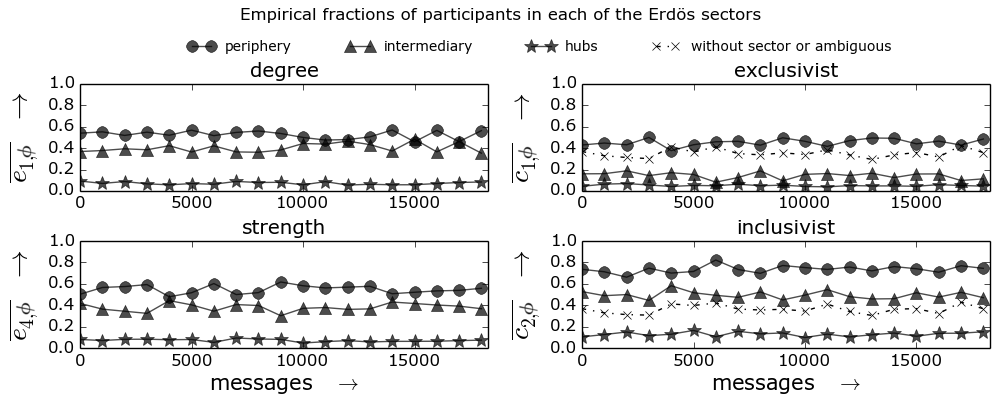
\includegraphics[width=\textwidth]{figs/InText-WLAU-S1000__}
\caption{Stability of Erd\"os sector sizes.
Fractions of participants derived from degree and strength criteria, $E_1$ and $E_4$ described in Section~\ref{sectioning}, are both on the left.
Fractions derived from the exclusivist $C_1$ and the inclusivist $C_2$ compound criteria are shown in the plots to the right.
The ordinates $\overline{e_{\gamma,\phi}}=\frac{|e_{\gamma,\phi}|}{N}$ denote the fraction of participants in sector $\phi$ through criterion $E_\gamma$
and, similarly, $\overline{c_{\delta,\phi}}=\frac{|c_{\delta,\phi}|}{N}$ denotes the fraction of participants in sector $\phi$ through criterion $C_\delta$.
The article~\cite{stab} bring a systematic collection of such timeline figures with all simple and compound criteria specified in Section~\ref{sectioning}, with results for networks from Facebook, Twitter and Participabr.}
\begin{flushleft}\footnotesize
Source: By the author.\
\end{flushleft}
\label{fig:sectIL}
\end{figure*}


\begin{table}[h]
\caption{Distribution of activity among participants.
The first column shows the percentage of messages sent by the most active participant. The column for the first quartile ($Q_1$) gives the minimum percentage of participants responsible for at least 25\% of total messages with the actual percentage in parentheses. Similarly, the column for the first three quartiles $Q_3$ gives the minimum percentage of participants responsible for 75\% of total messages.
The last decile $D_{-1}$ column shows the maximum percentage of participants responsible for 10\% of messages.}
\begin{center}
\begin{tabular}{ l ||  c | c | c | c }
\hline
list & hub & $ Q_1 $ & $ Q_3 $ & $D_{-1}$ \\ \hline\hline
LAU & 2.78  & 1.19 (26.35\%)  & 13.12 (75.17\%)  & 67.32 (-10.02\%) \\
LAD & 4.00  & 1.03 (26.64\%)  & 11.91 (75.18\%)  & 71.14 (-10.03\%) \\
MET & 11.14  & 1.02 (34.07\%)  & 8.54 (75.64\%)  & 80.49 (-10.02\%) \\
CPP & 14.41  & 0.29 (33.24\%)  & 4.18 (75.46\%)  & 83.65 (-10.04\%) \\\hline

\end{tabular}
\end{center}
\begin{flushleft}\footnotesize
Source: By the author.\
\end{flushleft}
\label{autores}
\end{table}


\subsection{Stability of principal components}\label{prevalence}
%The topology was analyzed using standard, well-established metrics of centrality and clustering.
%We also introduced symmetry metrics given the evidence of their importance in social contexts~\cite{newmanEvolving}.
%The contribution of each metric to the variance is very similar for all the networks and along time.

The principal components of the participants are very stable in the topological space,
i.e. in the space of network metrics.
Table~\ref{tab:pcainin} exemplifies the formation of principal components by providing the averages over non-overlapped activity snapshots of a network. The most important result of this application of PCA, the stability of principal components, is underpinned by the very small dispersion of the contribution of each metric to each principal component.
%The contribution of each metric to the
%principal components presents
%very small standard deviation.

\begin{table}[!h]
\caption{Loadings for the 14 metrics into the principal components for the MET list, $1000$ messages in 20 disjoint positions. The clustering coefficient (cc) appears as the first metric in the table, followed by 7 centrality metrics and 6 symmetry-related metrics. Note that the centrality measurements, including degrees, strength and betweenness centrality, are the most important contributors for the first principal component, while the second component is dominated by symmetry metrics. The clustering coefficient is only relevant for the third principal component. The three components have in average more than 85\% of the variance.
The low standard deviation $\sigma$ implies that the principal components are considerably stable.}
\footnotesize
\begin{center}
\begin{tabular}{| l || c | c | c | c | c | c |}\cline{2-7}
\multicolumn{1}{c|}{} & \multicolumn{2}{c|}{PC1}          & \multicolumn{2}{c|}{PC2} & \multicolumn{2}{c|}{PC3}  \\\cline{2-7}\multicolumn{1}{c|}{} & $\mu$            & $\sigma$ & $\mu$         & $\sigma$ & $\mu$ & $\sigma$  \\\hline
$cc$ &                     0.89  & 0.59  & 1.93  & 1.33  & {\bf 21.22}  & 2.97 \\\hline
$s$ &              {\bf 11.71}  & 0.57  & 2.97  & 0.82  & 2.45  & 0.72 \\
$s^{in}$ &         {\bf 11.68}  & 0.58  & 2.37  & 0.91  & 3.08  & 0.78 \\
$s^{out}$ &        {\bf 11.49}  & 0.61  & 3.63  & 0.79  & 1.61  & 0.88 \\
$k$ &              {\bf 11.93}  & 0.54  & 2.58  & 0.70  & 0.52  & 0.44 \\
$k^{in}$ &         {\bf 11.93}  & 0.52  & 1.19  & 0.88  & 1.41  & 0.71 \\
$k^{out}$ &        {\bf 11.57}  & 0.61  & 4.34  & 0.70  & 0.98  & 0.66 \\
$bt$ &             {\bf 11.37}  & 0.55  & 2.44  & 0.84  & 1.37  & 0.77 \\\hline
$asy$ &                    3.14  & 0.98  & {\bf 18.52}  & 1.97  & 2.46  & 1.69 \\
$\mu^{asy}$              & 3.32  & 0.99  & {\bf 18.23}  & 2.01  & 2.80  & 1.82 \\
$\sigma^{asy}$           & 4.91  & 0.59  & 2.44  & 1.47  & {\bf 26.84}  & 3.06 \\
$dis$                    & 2.94  & 0.88  & {\bf 18.50}  & 1.92  & 3.06  & 1.98 \\
$\mu^{dis}$              & 2.55  & 0.89  & {\bf 18.12}  & 1.85  & 1.57  & 1.32 \\
	$\sigma^{dis}$           & 0.57  & 0.33  & 2.74  & 1.63  & {\bf 30.61}  & 2.66 \\\hline\hline
$\lambda$                & 49.56 & 1.16  & 27.14  & 0.54  & 13.25  & 0.95 \\
\hline\end{tabular}
\end{center}

\label{tab:pcainin}
\begin{flushleft}\footnotesize
Source: By the author.\
\end{flushleft}
\end{table}

The first principal component is an average of centrality metrics:
degrees, strengths and betweenness centrality.
On one hand, the similar relevance of all centrality metrics is not surprising since they are highly correlated,
e.g. degree and strength have Spearman correlation coefficient $\in [0.95,1]$ 
and Pearson coefficient $\in [0.85,1)$ for window sizes greater than a thousand messages.
On the other hand, each of these metrics is related to a different participation characteristic,
and their equal relevance for variability,
as measured by the principal component, is noticeable.
Also, this suggests that these centrality metrics 
are equally adequate for characterizing the networks
and the participants.

\begin{figure} 
\centering
%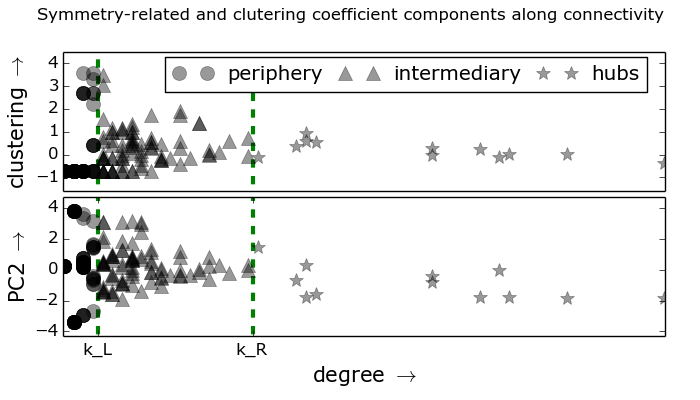
\includegraphics[width=.6\textwidth,height=10cm]{figs/im13PCAPLOT__}
 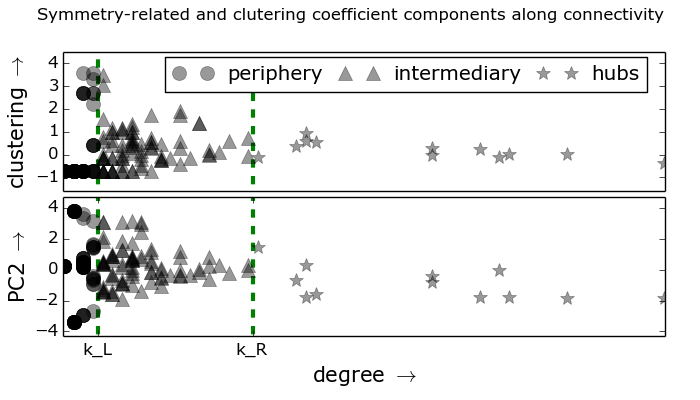
\includegraphics[width=.45\textwidth]{figs/im13PCAPLOT__}
\caption{The first plot highlights the well-known pattern of degree versus clustering coefficient, characterized by the higher clustering coefficient of lower degree vertices.
 The second plot shows the greater dispersion of the symmetry-related ordinates dominant in the second principal component (PC2).
 This larger dispersion suggests that symmetry-related metrics are more powerful,
 for characterizing interaction networks than the clustering coefficient,
 especially for hubs and intermediary vertices.
 This figure reflects a snapshot of the LAU list with 1000 contiguous messages.}

 %Similar structures were observed in all window sizes $ws\;\in\;[500,10000]$, in networks derived from email lists,
 %and in networks from Facebook, Twitter and Participabr,
 %which suggests a common relationship between the metrics of degrees, strengths and betweenness centrality,
 %the symmetry-related metrics and clustering coefficient.}
 \label{fig:sym}
 \begin{flushleft}\footnotesize
Source: By the author.\
\end{flushleft}
\end{figure}

According to Table~\ref{tab:pcainin} and Figure~\ref{fig:sym},
dispersion is larger in symmetry-related metrics than in clustering coefficient.
% As expected from basic complex network theory, peripheral vertices have low values of centrality metrics and larger dispersion with regard to the clustering coefficient.
% %The scatter plot in the third system of Figure~\ref{fig:sym},
% %where all metrics are considered and there is a greater dispersion
% %with respect to the ordinates,
% This reflects in the relevance of the symmetry-related metrics.
We conclude that the symmetry metrics are more powerful, in terms of dispersion in the topological metrics space, in characterizing interaction networks and their participants, than the clustering coefficient, especially for hubs and intermediary vertices (peripheral vertices have larger dispersion with regard to the clustering coefficient).
Interestingly, the clustering coefficient is always combined
with the standard deviation of the asymmetry and disequilibrium
of edges $\sigma^{asy}$ and $\sigma^{dis}$ in the third principal component.

%These results are also reported for 12 networks from Facebook, Twitter and Participabr
%in Section~\ref{si:ext} of the Supporting Information document.
Similar results are presented in~\cite{stab} for other email lists and interaction networks. A larger variability was found for the latter networks,
which motivated the use of interaction networks derived from email lists for benchmarking.

%the overall behavior was maintained in that centrality measurements 
%were found prevalent in the first principal component,
%followed by symmetry-related metrics on the second principal
%component and then clustering coefficient on the third principal component.
%Similar results are presented in Sections~\ref{si:pcat} and~\ref{si:ext}
%of the Supporting Information document for other email lists and other interaction networks,
%with the consideration of strategic combinations of metrics.

\subsection{Types from Erd\"os sectors}\label{sec:pty}


Assigning a type to a participant raises important issues about the scientific cannon for human types and the potential for stigmatization and prejudice. The Erd\"os sector to which a participant belongs can be regarded as implying a social type for this participant.
In this case, the type of a participant changes both along time and as different networks are considered, despite the stability of the network. Therefore, the potential for prejudice of such participant typology is attenuated~\cite{adorno}. In other words, an individual is a hub in a number of networks and peripheral in other networks, and even within the same network he/she most probably changes type along time~\cite{animacoes}.

The importance of this issue can be grasped by the consideration of static types derived from quantitative criteria. For example, in email lists with a small number of participants, the number of threads has a negative correlation with the number of participants.
When the number of participants exceeds a threshold, the number of threads has a positive correlation with the number of participants.
This finding is illustrated in Figure~\ref{fig:nmgamma3d}
and can also be observed in Table~\ref{tab:genLists}.
The assignment of types to individuals, in this latter case,
has more potential for prejudice because
the derived participant type is static and
one fails to acknowledge that
human individuals are not immutable entities.

Further observations regarding the Erd\"os sectors
and the implicit participant types were made, which are consistent with the literature~\cite{barabasiEvo}: 1) hubs and intermediary participants usually have intermittent activity, and stable activity was found only in smaller communities. For instance, the MET list had stable hubs while LAU, LAD and CPP exhibited intermittent hubs.
2) Network structure seems to be most influenced by the
activity of intermediary participants as they have less extreme
roles than hubs and peripheral participants and
can therefore connect to the sectors and other participants 
in a more selective and explicit manner.




%Moreover, such typology of participants bridges exact and human sciences and may 
%be enriched with concepts from other typologies,
%such as Meyer-Briggs, Pavlov or the authoritarian types of the F-Scale~\cite{adorno}.

%We analyzed the temporal evolution of the networks
%using visualization
%tools developed for this research~\cite{rcText,versinus}
%and inspected raw data.

%dictated (or revealed) by the
%(e.g. stable or intermittent patterns of activity and preferential communication
%with hubs or periphery)

%of both hubs and peripheral vertices
%have the trivial facets of interacting 
%
%
%
%\begin{itemize}
%\item Typically, the activity of hubs is trivial: they interact as much as possible, in every occasion with everyone.
%The activity of peripheral vertices also follows a simple pattern: they interact very rarely, in very few occasions.
%Therefore, intermediary vertices seem responsible for the network structure.
%Intermediary vertices may exhibit preferential communication to peripheral, intermediary, or hub vertices; can be marked by stable communication partners; can involve stable or intermittent patterns of activity, to point just a few examples of this greater variety of roles.
%%\item Some of the most active participants receive many responses with relative few messages sent, and rarely are top hubs.
%%These seem as authorities and contrast with participants that respond much more than receive responses.
%%\item The most obvious community structure, as observed by a high clustering coefficient, i.e. members know each other often, is found mostly in peripheral and intermediary sectors.
%\end{itemize}

%Within networks as the whole objects of analysis,
%we were able to observe a peculiar correlation pattern 
%between the number of threads and the number of participants.
\begin{figure}
\centering
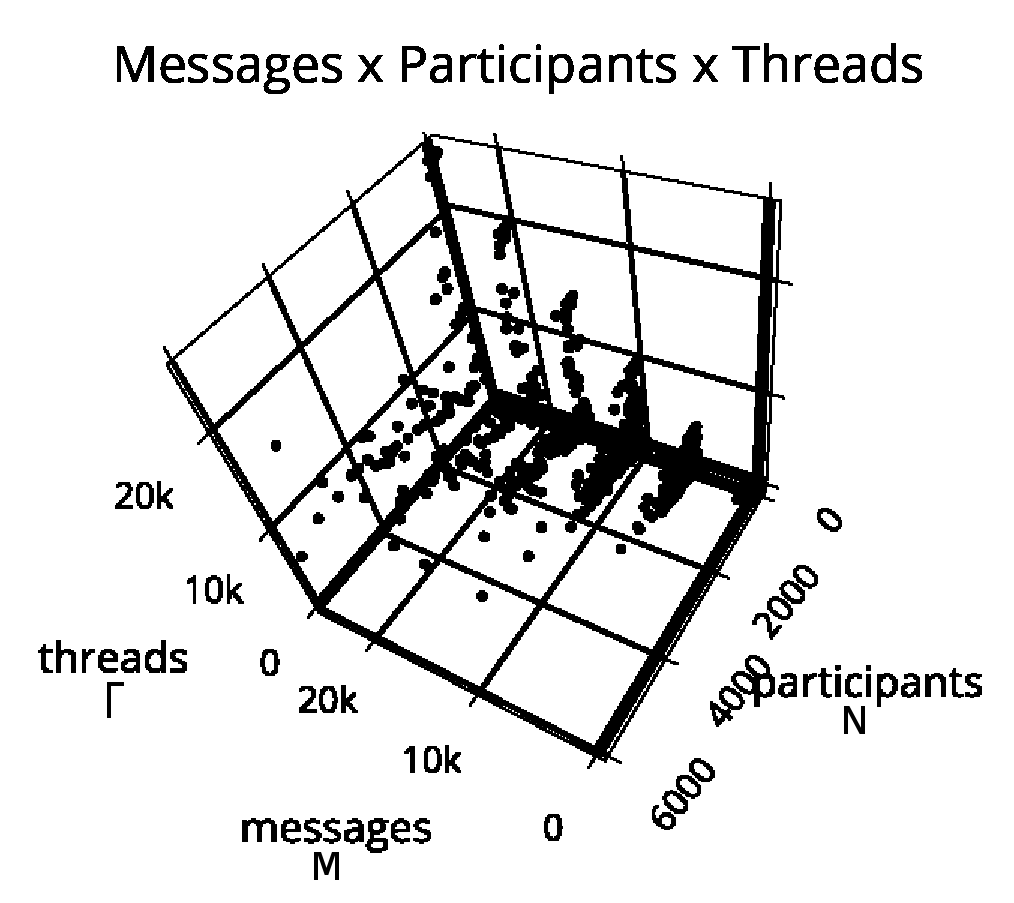
\includegraphics[trim={0 0 0 1cm},clip,width=.7\columnwidth]{figs/mpgamma2_}
\caption{A scatter plot of number of messages $M$ versus number of participants $N$ versus number of threads $\Gamma$ for 140 email lists.
Highest $\Gamma$ is associated with low $N$.
The correlation between $N$ and $\Gamma$ is negative for low values of $N$ but positive otherwise.
This negative correlation between $N$ and $\Gamma$ can also be observed in Table~\ref{tab:genLists}.
Accordingly, for $M=20000$ messages, this inflection
of correlation was found around $N=1500$, while CPP, LAU, LAD, MET lists 
present smaller networks.}
\begin{flushleft}\footnotesize
Source: By the author.\
\end{flushleft}
\label{fig:nmgamma3d}
\end{figure}


%\section{Discussion}
% given the results, and before reaching the conclusions
% what to say?
% --> what is the overall knowledge derived from the results
% --> what are the limitations of this knowledge and of individual results
% --> how should this results carry on is on the next sections.
%\subsection{Consecutive scientific research}
% --> research
% textual diferences
% audiovisualization of data
% typologies, sociological critical theory, social psychology

%\subsection{Technological applications}
% --> technological 
% resources categorization and recommendation
% document creation
% ontologies for the semantic web

%\subsection{Experimental and theoretical aspects of the research}
% --> methods
% Exploratory?
% Hypothesis testing?
% --> contributions
% verifiable
% knowledge
% contextualization in the academic knowledge

\subsection{Implications of the main findings}\label{sec:impl}
The findings reported in this thesis arose from an exploratory procedure to visually inspect the networks and to analyze considerable amounts of interaction networks data.
% deriving from email lists and also from other networks.
While this procedure has certainly an ad hoc nature, the statistics in the data are sufficiently robust for important features from these interaction networks to be extracted.
Temporal stability, in the sense that interaction networks could be considered as stationary time series, is the most important feature. Also relevant is the significant stability found on the principal components, on the fraction of participants in each Erd\"os Sector and on the activity along different timescales. In fact, these findings confirm our initial hypothesis - based on the literature~\cite{newmanBook} - that interaction networks should exhibit some stability traces. The potential generality of these findings is suggested by the analysis of networks derived from diverse systems, with interaction networks from public email lists serving as proper benchmarks. Indeed, with such benchmarks one can compare any social network system. Furthermore, this analysis enables us to establish an outline of human interaction networks. It takes the hub, intermediary and periphery sectors out of the scientific folklore and into classes drawn from quantitative criteria. It enables the conception of non-static human types derived from natural properties.

 
We envisage that the knowledge generated in the analysis may be exploited in applications where the type of each participant and the relative proportion of participants in each sector can be useful metadata. Just by way of illustration, this could be applied in semantic web initiatives, given that the Erd\"os sectorialization is static in a given snapshot. These results are also useful for classifying resources, e.g. in social media, and for resources recommendation to users~\cite{opa}. 
Finally, the knowledge acquired with a quantitative treatment of the whole data may help guide the creation through collective processes of documents to assist in participatory democracy.

 
Perhaps the most outreaching implications are related to sociological consequences. The results expose a classification of human individuals which is directly related to the concentration of wealth and based on natural laws. The derived human typology changes over different systems and over time in the same system, which implies a negation of the absolute concentration of wealth. Such concentration exists but changes across different wealth criteria and with time. Also, the hubs stand out as dedicated, sometimes enslaved,
components of the social system. The peripheral participants have very limited interaction with the network. This suggests that intermediary participants tend to dictate structure, legitimate the hubs and stand out as authorities.

 
With regard to the limitations of our study, one should emphasize that not all types of human interaction networks were analyzed. Therefore, the plausible generalization of properties has to be treated with caution, as a natural tendency of such systems and not as a rule. Also, the stable properties in the networks were not explored to the limit, which leaves many open questions. For example, what are the maximum and minimum sizes of the networks for which they hold? What is the outcome of PCA when more metrics are considered? What is the granularity in which the activity along the timescales is preserved? Do the findings reported also apply to other systems, beyond human networks?
 
  % TTM find
  \section{Text-related results and discussion}\label{sec:tresults}
  % Aqui será necessária uma Introdução a este novo tipo de resultado.

  The most important result of including textual metrics in our analysis is the
  statistical evidence of differentiation of each Erd\"os sector with respect to the texts produced.
  This conclusion can be reached by observing the differences in the measurements of textual features in
  each sector, and is supported on firm theoretical grounds by using the adapted Kolmogorov-Smirnov test presented in Section~\ref{sec:ks}.
  % derived from the kolmogorov-smirnov test adaptation
  Other relevant results are:
  \begin{itemize}
\item the identification of patterns in the frequency of use of nouns, adverbs, sizes of words, depth of Wordnet synsets and other linguistic traces, by different types of participants in the Erd\"os sectors. We did not find in the literature any indication for such values; we believe it is useful to report e.g. that about 15\% of the characters are spaces and that nouns often account for more than 25\% of the words.
These values are available in~\cite{textTables} and not in the body of the text,
		  since the focus in this thesis is the evidence that texts from distinct sectors differ.
\item Evidence of what is different in the texts produced by each of the Erd\"os sectors. For example: hubs were found to use more contractions,
more common words, and less punctuation if compared to the rest of the network,
especially the peripheral sector.
In general, the rise or fall of a text-related metric is not relevant or is monotonic along connectivity,
but some of them reach extreme values in the intermediary sector.
% Comparative insights by means of statistics from email lists, the King James Bible and Shakespeare, which are often regarded as pillars of the English language. TTM
\end{itemize}

	The next sections summarize results of immediate interest
and further insights can be obtained by skimming through
the tables and figures of~\cite{stab,textTables} and the Conclusions chapter.
We illustrate with just one table of each kind,
and from networks obtained with 2000 messages.
In~\cite{textTables} we display tables for various networks.
In the same document, we relate the email lists to each numerical
TAG in the tables of the following sections.
The scale of 1000 and 2000 messages was chosen for deriving results,
as the networks in this scale are found to have stable topological structure,
as described in Section~\ref{subsec:pih}.
The findings with 1000 messages are the same as with 2000 messages,
and there are many tables.
This motivated the exclusion of the tables with measurements in
networks of 1000 messages.

\subsection{General characteristics of activity distribution among sectors}\label{sec:gen}
Before we dig into the findings derived from text-related measurements,
let us look once more at the general structure of these networks,
now giving emphasis on the activity of the sectors.
In almost all our observations,
the peripheral sector was responsible for starting most of the discussion threads,
i.e. for sending messages to the list which are not replies.
This is surprising since the peripheral sector is responsible for fewer messages. It suggests complementarity between peripheral diversity and hub specialization, which, on its turn, deepens the understanding of the interaction network as a meaningful system. 
These assertions are condensed in Table~\ref{geralListas}.
Less often, the intermediary sector is responsible for the largest number of messages and of threads.
Also meaningful is that the hubs sector is responsible for most of the messages, which is not obvious: hub participants are far more active but way less numerous. Interestingly, in such a setting where every characteristic differs with respect to
distinct sectors, there was no evidence of difference on the size of the threads started by each sector.
\begin{table}[h!]
\begin{center}
\caption{Distribution of participants, messages and threads among each Erd\"os sector ({\bf p.} for periphery, {\bf i.} for intermediary, 
    {\bf h.} for hubs) in a total timespan of 0.72 years (from 2003-11-30T20:21:32 to 2004-08-19T18:11:24). $N$ is the number of participants, $M$ is the number of messages, $\Gamma$ is the number of threads, and $\gamma$ is the number of messages in a thread.
    The \% denotes the usual `per cent' with respecto to the total quantity ($100\%$ for {\bf g.})
    while $\mu$ and $\sigma$ denote mean and standard deviation. TAG of list in the Appendix~\ref{ap:texttop}: 10}\label{geralListas}    
\begin{tabular}{| l || c | c | c | c |}\hline
 & {\bf g.} & {\bf p.} & {\bf i.} & {\bf h.} \\\hline\hline
$N$ & 131  & 80  & 46  & 5 \\
$N_{\%}$ & 100.00  & 61.07  & 35.11  & 3.82 \\\hline
$M$ & 1000.00  & 136.00  & 361.00  & 503.00 \\
$M_{\%}$ & 100.00  & 13.60  & 36.10  & 50.30 \\\hline
$\Gamma$ & 292.00  & 76.00  & 147.00  & 69.00 \\
$\Gamma_{\%}$ & 100.00  & 26.03  & 50.34  & 23.63 \\\hline
$\frac{\Gamma}{M}\%$ & 29.20  & 55.88  & 40.72  & 13.72 \\
$\mu(\gamma)$ & 2.74  & 2.76  & 2.81  & 2.58 \\
$\sigma(\gamma)$ & 0.44  & 0.43  & 0.39  & 0.49 \\\hline
\end{tabular}
\end{center}
\begin{flushleft}
		Source: Prepared by the authors.\
\end{flushleft}
\end{table}


%Also, comparing lists with a fixed number of messages,
%the number of threads created seem to increase as the number of participants decrease.

\subsection{Evidence that the texts from Erd\"os sectors differ}\label{subsec:di}
Results from our adaptation of the Kolmogorov-Smirnov test (see Section~\ref{sec:ks})
present strong evidence
that the texts produced by each sector are different.
Tables~\ref{tab:kolTok}-\ref{tab:kolPctInter}
illustrate three results:
\begin{itemize}
 \item There is statistical evidence that the textual production of the Erd\"os sectors is different.
	 This can be noticed from the high values of $c'$ on these tables, above reference values used for the acceptance of the null hypothesis (the null hypothesis being that the probability distributions generating the samples are the same). Also, we regarded as non-negligible the values often above 0.1 for the Kolmogorov-Smirnov statistics (the maximum difference between the cumulative distributions), which we recognized as relevant for assuming differences in the underlying distributions in our study (see Section~\ref{sec:ks}).
  \item Intermediary sectors sometimes exhibit greater differences 
from periphery and hubs than these extreme sectors between themselves 
(Tables~\ref{tab:kolTok} and~\ref{tab:kolSub}).
This differentiation of the three sectors is an indication that the Erd\"os Sectioning described in Section~\ref{sectioning} reveals meaningful sectors of the networks.
 \item The evidence of difference (as measured by $c'$) between sectors on the same network (Tables~\ref{tab:kolTok}-\ref{tab:kolPct}) is often larger than found between the same sector from distinct networks (Tables~\ref{tab:kolSubInter}-\ref{tab:kolPctInter}).
 \end{itemize}

 In Tables~\ref{tab:kolTok}-\ref{tab:kolPct}, there are two measurements for each pair of sectors.
 The top value is $c'$ while the bottom value is the Kolmogorov-Smirnov statistic.
 In Tables~\ref{tab:kolSubInter}-\ref{tab:kolPctInter} only $c'$ values are shown to illustrate
 that the measurements found between networks are comparable to measurements found between sectors of a same network.
 \begin{table}[h!]
\begin{center}
	\caption{Measurements of $c'$ and the KS statistic related to sizes of tokens between the Erd\"os sectors and the whole network. The abbreviations are: g for global, p for peripheral, i for intermediary, h for hubs. See Section~\ref{sec:ks} for and explanation of the measures and Section~\ref{subsec:di} for discussion. TAG of list in~\cite{textTables}: 6}
\label{tab:kolTok}
\begin{tabular}{| l || c | c | c | c | c | c |}\hline
{\bf } & {\bf p-g} & {\bf i-g} & {\bf h-g} & {\bf p-i} & {\bf p-h} & {\bf i-h} \\\hline\hline
$c'$ & 4.327  & 17.168  & 7.851  & 18.907  & 7.833  & 15.540 \\
KS & 0.014  & 0.115  & 0.044  & 0.129  & 0.045  & 0.129 \\\hline
\end{tabular}
\begin{flushleft}
Source: By the author.\
\end{flushleft}
\end{center}
\end{table}

 \begin{table}[h!]
\begin{center}
\caption{Measurements of $c'$ and the KS statistic related to sizes of known words between the Erd\"os sectors and the whole network. The abbreviations are: g for global, p for peripheral, i for intermediary, h for hubs. See Section~\ref{sec:ks} for and explanation of the measures and Section~\ref{subsec:di} for discussion. TAG of list in~\cite{textTables}: 1}
\begin{tabular}{| l || c | c | c | c | c | c |}\hline
{\bf } & {\bf p-g} & {\bf i-g} & {\bf h-g} & {\bf p-i} & {\bf p-h} & {\bf i-h} \\\hline\hline
$c'$ & 5.904  & 5.264  & 5.549  & 9.547  & 7.073  & 4.058 \\
KS & 0.043  & 0.040  & 0.150  & 0.083  & 0.193  & 0.111 \\\hline
\end{tabular}
\begin{flushleft}
Source: By the author.\
\end{flushleft}
\end{center}
\end{table}

 \begin{table}[h!]
\begin{center}
\caption{Measurements of $c'$ and the KS statistic related to sizes of sentences between the Erd\"os sectors and the whole network. The abbreviations are: g for global, p for peripheral, i for intermediary, h for hubs. See Section~\ref{sec:ks} for and explanation of the measures and Section~\ref{subsec:di} for discussion. TAG of list in~\cite{textTables}: 2}
\begin{tabular}{| l || c | c | c | c | c | c |}\hline
{\bf } & {\bf p-g} & {\bf i-g} & {\bf h-g} & {\bf p-i} & {\bf p-h} & {\bf i-h} \\\hline\hline
$c'$ & 0.733  & 2.077  & 2.834  & 1.642  & 2.589  & 4.139 \\
KS & 0.020  & 0.038  & 0.059  & 0.048  & 0.080  & 0.097 \\\hline
\end{tabular}
\begin{flushleft}\footnotesize
Source: By the author.\
\end{flushleft}
\end{center}
\end{table}


 \begin{table}[h!]
\begin{center}
\caption{Measurements of $c'$ and the KS statistic related to the frequency of use of adjectives between the Erd\"os sectors and the whole network. The abbreviations are: g for global, p for peripheral, i for intermediary, h for hubs. See Section~\ref{sec:ks} for and explanation of the measures and Section~\ref{subsec:di} for discussion. TAG of list in~\cite{textTables}: 3}
\begin{tabular}{| l || c | c | c | c | c | c |}\hline
{\bf } & {\bf p-g} & {\bf i-g} & {\bf h-g} & {\bf p-i} & {\bf p-h} & {\bf i-h} \\\hline\hline
$c'$ & 0.461  & 0.564  & 0.617  & 0.385  & 0.800  & 0.986 \\
KS & 0.011  & 0.010  & 0.010  & 0.011  & 0.021  & 0.020 \\\hline
\end{tabular}
\begin{flushleft}\footnotesize
Source: By the author.\
\end{flushleft}
\end{center}
\end{table}

 \begin{table}[h!]
\begin{center}
\caption{Measurements of $c'$ and the KS statistic between the Erd\"os sectors and the whole network. The abbreviations are: g for global, p for peripheral, i for intermediary, h for hubs. See Section~\ref{sec:ks} for and explanation of the measures and Section~\ref{subsec:di} for discussion.}\label{tab:kolSub}
\begin{tabular}{| l || c | c | c | c | c | c |}\hline
{\bf } & {\bf p-g} & {\bf i-g} & {\bf h-g} & {\bf p-i} & {\bf p-h} & {\bf i-h} \\\hline\hline
$c'$ & 0.642  & 1.791  & 6.936  & 1.007  & 6.970  & 7.510 \\
KS & 0.023  & 0.067  & 0.537  & 0.044  & 0.560  & 0.607 \\\hline
\end{tabular}
\begin{flushleft}
Source: Prepared by the author.\
\end{flushleft}
\end{center}
\end{table}

 \begin{table}[h!]
\begin{center}
	\caption{Measurements of $c'$ and the KS statistic related to the frequency of use of punctuations between the Erd\"os sectors and the whole network. The abbreviations are: g for global, p for peripheral, i for intermediary, h for hubs. See Section~\ref{sec:ks} for and explanation of the measures and Section~\ref{subsec:di} for discussion. TAG of list in~\cite{textTables}: 8}\label{tab:kolPct}
\begin{tabular}{| l || c | c | c | c | c | c |}\hline
{\bf } & {\bf p-g} & {\bf i-g} & {\bf h-g} & {\bf p-i} & {\bf p-h} & {\bf i-h} \\\hline\hline
$c'$ & 1.380  & 3.583  & 2.894  & 1.718  & 2.871  & 5.398 \\
KS & 0.039  & 0.069  & 0.046  & 0.054  & 0.085  & 0.114 \\\hline
\end{tabular}
\begin{flushleft}
Source: By the author.\
\end{flushleft}
\end{center}
\end{table}

 \begin{table}
  \centering
  \caption{$c'$ values for substantives. Comparison of the same sector between lists, each author is an observation. See subsection~\ref{subsec:di} for discussion and directions.}
    \small
\setlength{\tabcolsep}{.06667em}
  \begin{tabular}{|l|| c|c|c|c|c|c|}\hline
& CPP-LAD & CPP-LAU & CPP-ELE & LAD-LAU & LAD-ELE & LAU-ELE \\\hline
P & 1.35 & 4.05 & 5.80 & 3.00 & 5.41 & 4.94 \\\hline
I & 1.27 & 0.78 & 4.01 & 0.84 & 3.84 & 3.94 \\\hline
H & 0.98 & 1.94 & 3.17 & 1.32 & 3.82 & 4.47 \\\hline
  \end{tabular}
\begin{flushleft}
		Source: Prepared by the authors.\
\end{flushleft}
  \label{tab:kolSubInter}
\end{table}

\begin{table}
  \centering
  \caption{$c'$ values for adjectives. Comparison of the same sector between lists, each author is an observation. See subsection~\ref{subsec:di} for discussion and directions.}
    \small
\setlength{\tabcolsep}{.06667em}
  \begin{tabular}{|l|| c|c|c|c|c|c|}\hline
 & CPP-LAD & CPP-LAU & CPP-ELE & LAD-LAU & LAD-ELE & LAU-ELE \\\hline
P & 0.44 & 0.34 & 2.57 & 0.20 & 2.32 & 2.37 \\\hline
I & 0.74 & 0.99 & 3.72 & 0.32 & 3.37 & 3.10 \\\hline
H & 0.26 & 0.32 & 3.72 & 0.29 & 4.36 & 4.24 \\\hline
  \end{tabular}
\begin{flushleft}
		Source: Prepared by the authors.\
\end{flushleft}
  \label{tab:kolAdjInter}
\end{table}

\begin{table}
  \centering
  \caption{$c'$ values for stopwords. Comparison of the same sector between lists, each author is an observation. See subsection~\ref{subsec:di} for discussion and directions.}
    \small
\setlength{\tabcolsep}{.06667em}
  \begin{tabular}{|l|| c|c|c|c|c|c|}\hline
 & CPP-LAD & CPP-LAU & CPP-ELE & LAD-LAU & LAD-ELE & LAU-ELE \\\hline
P & 3.31 & 3.26 & 6.68 & 0.57 & 5.36 & 5.41 \\\hline
I & 1.45 & 1.08 & 5.16 & 0.91 & 5.00 & 4.92 \\\hline
H & 0.98 & 0.68 & 4.35 & 1.05 & 4.73 & 5.01 \\\hline
  \end{tabular}
\begin{flushleft}
		Source: Prepared by the authors.\
\end{flushleft}
  \label{tab:kolSwInter}
\end{table}

\begin{table}
  \centering
  \caption{$c'$ values for punctuations/char. Comparison of the same sector between lists, each author is an observation. See subsection~\ref{subsec:di} for discussion and directions.}
    \small
\setlength{\tabcolsep}{.06667em}
  \begin{tabular}{|l|| c|c|c|c|c|c|}\hline
 & CPP-LAD & CPP-LAU & CPP-ELE & LAD-LAU & LAD-ELE & LAU-ELE \\\hline
P & 5.74 & 4.88 & 8.28 & 2.23 & 5.37 & 6.60 \\\hline
I & 3.23 & 2.49 & 4.16 & 0.96 & 3.40 & 3.51 \\\hline
H & 2.49 & 1.87 & 4.02 & 1.36 & 3.05 & 3.71 \\\hline
  \end{tabular}
\begin{flushleft}
		Source: Prepared by the authors.\
\end{flushleft}
  \label{tab:kolPctInter}
\end{table}
 


 \FloatBarrier
 \subsection{What differs and how the texts from the sectors differ}
 In the next sections we will look through text-related measurements
 and summarize the findings about what might be different in
 the textual features of the sectors.
 One should keep in mind that our core result is the evidence that
 the texts from distinct sectors differ.
 The following discussion of what differs and how it differs
 is interesting but is both derived from less strong statistical evidence and less crucial for our current stage of researching these structures.
 Nonetheless, for the sake of clarity, we state the main findings in this respect:
 \begin{itemize}
\item Peripherals were found to use more nouns while hubs use more verbs and adverbs. The fraction of adjectives did not change as irrefutably with respect to connectivity, but given that nouns are more numerous in the periphery sector, there are more adjectives per noun in the hubs sector texts.
\item Sentences and messages were found smaller in the more connected sectors although punctuation was more incident in the less connected sectors.
\item The differences found in analyzing Wordnet synset hypernyms were found less well behaved. Often, the sectors exhibit noticeable differences but greater and smaller incidences are found in all sectors (but in different networks). Some of these incidences are more systematic and this analysis assisted by Wordnet is the only semantic analysis we made, which is why we included these results.
\end{itemize}
Appendix~\ref{ap:textd} presents tables with counts for larger incidence in each sector throughout the networks. In the following discussion we display example tables for each set of measurements.
In the measurements derived from synset hypernyms the example tables were less meaningful because of the greater variability and therefore we present the counts of greater incidence directly.
In any case, the measurements for each of the networks are in~\cite{textTables}.
The analysis of the measurements we obtained
is not trivial because of the number of different measures
and because differences in measurements are not obviously relevant.
Furthermore, there is too much variation among networks
which renders worthless the usual global measurements such as mean and variance when obtained from all the systems at once.
In order to obtain consistent results, we considered \emph{weak evidence of difference} in sectors in a network
if maximum measure is at least 10\% greater than minimum measure,
i.e. $\frac{maximum\;measure}{minumum\;measure}>1.1$.
We considered \emph{evidence of difference} in sectors in a network if
$\frac{maximum\;measure}{minumum\;measure}>1.2$.
When 
$\frac{maximum\;measure}{minumum\;measure}>1.5$, we considered \emph{strong evidence of difference}.
We then looked through each measure in all networks to reach compelling observations about the
differences of sectors through all networks.
Instead of the counts of maximum incidences, we also performed a weighted count:
when the evidence was weak, the sector received an add of $0.5$ in the weighted count;
then the evidence was strong, the sector received an add of $2$ in the weighted count.
The results were qualitatively the same, so we omit the tables with weighted counts.
Also useful here is the definition of lower sectors (peripheral and intermediary),
upper sectors (intermediary and hubs) and extreme sectors (peripheral and hubs).
We should also point when measurements peak often at the intermediary sector,
be it a maximum or minimum peak.

The tables that follow have terms for measurements that might be immediately inferred,
but this depends on the background of the reader.
Therefore the terms are explicitly defined in Appendix~\ref{ap:msTerms}.
% We can summarize these results stating that the difference
% found between texts from distinct Erd\"os sectors
% is further evidenced.
% We can summarize these results stating that the difference
% found between the texts produced by the Erd\"os sectors
% are greater than the difference found between texts from different
% networks or from the same sector of different networks.

\subsection{Characters}\label{sec:cha}
Most often, peripheral and intermediary sectors use more digits, upper case letters and punctuation.
Hubs sectors were found to use more spaces in most cases. 
These results are illustrated in Table~\ref{tab:cha}.
\begin{table}[h!]
\begin{center}
\begin{tabular}{| l || c | c | c | c |}\hline
 & {\bf g.} & {\bf p.} & {\bf i.} & {\bf h.} \\\hline\hline
$chars$ & 1485813  & 552986  & 554328  & 378499 \\
$chars_{\%}$ & 100.00  & 37.22  & 37.31  & 25.47 \\\hline
$\frac{spaces}{chars}$ & 12.94  & 12.79  & 12.82  & 13.35 \\
$\frac{punct}{chars-spaces}$ & 9.54  & 10.53  & 10.15  & 7.20 \\
$\frac{digits}{chars-spaces}$ & 4.49  & 7.13  & 3.87  & 1.54 \\\hline
$\frac{letters}{chars-spaces}$ & 83.95  & 80.09  & 83.95  & 89.65 \\
$\frac{vowels}{letters}$ & 36.94  & 36.10  & 36.98  & 38.00 \\
$\frac{uppercase}{letters}$ & 4.49  & 4.60  & 4.68  & 4.07 \\\hline
\end{tabular}
\caption{Characters in each Erd\"os sector ({{\bf p.}} for periphery, {{\bf i.}} for intermediary, 
	{{\bf h.}} for hubs). TAG: 6}\label{tab:cha}
\end{center}
\end{table}

\FloatBarrier
% The total number of characters in ELE list,
% in the 20 thousand messages,
% is more than three times what other lists exhibited.
% This suggests peculiarities related to communication conventions and style (see Appendix~\ref{sec:materials}) and were found not related to topological features.

\subsection{Tokens and words}\label{subsec:tw}
%\begin{table}[h!]
\begin{center}
\begin{tabular}{| l || c | c | c | c |}\hline
 & {\bf g.} & {\bf p.} & {\bf i.} & {\bf h.} \\\hline\hline
$tokens$ & 17964  & 1539  & 6064  & 10361 \\
$tokens_{\%}$ & 100.00  & 8.57  & 33.76  & 57.68 \\
$tokens \neq$ & 15.21  & 32.16  & 25.89  & 18.02 \\\hline
$\frac{knownw}{tokens}$ & 36.48  & 35.74  & 38.03  & 35.69 \\
$\frac{knownw \neq}{knownw}$ & 8.62  & 24.73  & 15.31  & 10.84 \\\hline
$\frac{stopw}{knownw}$ & 11.43  & 10.00  & 11.71  & 11.47 \\
$\frac{punct}{tokens}$ & 23.73  & 22.35  & 22.82  & 24.47 \\
$\frac{contrac}{tokens}$ & 0.01  & 0.00  & 0.00  & 0.02 \\\hline
\end{tabular}
\caption{tokens in each Erd\"os sector ({{\bf p.}} for periphery, {{\bf i.}} for intermediary, 
    {{\bf h.}} for hubs).}
\end{center}
\end{table}

%The largest average size of tokens is from the most wordy list (ELE).
%This implies that is has more characters, tokens, and characters per token in comparison to the other lists. 
Hubs were found to use more contractions and stopwords, while the peripheral sectors exhibit greater incidence of punctuations among tokens.
Although the token diversity ($\frac{|tokens \neq|}{|tokens|}$) found in peripheral sector is greater,
this result has the masking artifact that the peripheral sector corpus is smaller, yielding a larger token diversity.
This can be noticed by the token diversity of the whole network, which is lower than in any of the sectors.
These results are exemplified in Table~\ref{tab:tokensInline}
where mean and variance were taken with respect to the length in characters of tokens, known words and stopwords.
\begin{table}[h!]
\begin{center}
\begin{tabular}{| l || c | c | c | c |}\hline
 & {\bf g.} & {\bf p.} & {\bf i.} & {\bf h.} \\\hline\hline
$tokens$ & 286232  & 146472  & 134852  & 4908 \\
$tokens_{\%}$ & 100.00  & 51.17  & 47.11  & 1.71 \\
$tokens \neq$ & 3.00  & 4.01  & 3.66  & 24.08 \\\hline
$\frac{knownw}{tokens}$ & 25.76  & 25.11  & 26.21  & 32.84 \\
$\frac{knownw \neq}{knownw}$ & 4.51  & 6.22  & 5.92  & 42.80 \\\hline
$\frac{stopw}{knownw}$ & 42.46  & 38.92  & 43.60  & 98.33 \\
$\frac{punct}{tokens}$ & 33.18  & 34.09  & 32.56  & 23.11 \\
$\frac{contrac}{tokens}$ & 0.16  & 0.10  & 0.18  & 1.67 \\\hline\hline
$\mu(\overline{tokens})$ & 3.19  & 3.10  & 3.26  & 3.65 \\
$\sigma(\overline{tokens})$ & 2.53  & 2.54  & 2.52  & 2.60 \\\hline
$\mu(\overline{knownw})$ & 4.89  & 4.69  & 5.06  & 5.50 \\
$\sigma(\overline{knownw})$ & 2.37  & 2.41  & 2.31  & 2.28 \\\hline
$\mu(\overline{knownw \neq})$ & 6.53  & 6.39  & 6.27  & 6.16 \\
$\sigma(\overline{knownw \neq})$ & 2.53  & 2.50  & 2.46  & 2.42 \\\hline
$\mu(\overline{stopw})$ & 2.83  & 2.83  & 2.83  & 2.81 \\
$\sigma(\overline{stopw})$ & 0.87  & 0.84  & 0.86  & 1.17 \\\hline
\end{tabular}
	\caption{Tokens in each Erd\"os sector ({{\bf p.}} for periphery, {{\bf i.}} for intermediary, {{\bf h.}} for hubs). TAG: 1}\label{tab:tokensInline}
\end{center}
\end{table}

\FloatBarrier
% medir para tamanhos equivalentes de texto TTM

% ELE and CPP both exhibit intermediaries 
% with the more frequent production of punctuation,
% less frequent production of known words, and
% the highest incidence of words with wordnet synsets among known words.
% This suggests some peculiarity in network structure,
% such as authorities in the intermediary sector of such networks,
% using smaller sentences and a more intensive use of jargons,
% as made explicit in the following sections.
% verificar isso e ver o que fazer

% Words with synsets,
% among known English words, are less frequent in hubs sector,
% evidencing the jargon and specialization of hubs.
% verificar, desenvolvar

%\begin{table}[h!]
\begin{center}
\begin{tabular}{| l || c | c | c | c |}\hline
 & {\bf g.} & {\bf p.} & {\bf i.} & {\bf h.} \\\hline\hline
$\mu(\overline{tokens})$ & 3.84  & 3.94  & 3.86  & 3.82 \\
$\sigma(\overline{tokens})$ & 2.99  & 3.10  & 2.96  & 2.99 \\\hline
$\mu(\overline{knownw})$ & 3.28  & 3.27  & 3.32  & 3.26 \\
$\sigma(\overline{knownw})$ & 1.81  & 1.86  & 1.80  & 1.81 \\\hline
$\mu(\overline{knownw \neq})$ & 5.12  & 4.35  & 4.92  & 4.98 \\
$\sigma(\overline{knownw \neq})$ & 2.20  & 2.22  & 2.25  & 2.15 \\\hline
$\mu(\overline{stopw})$ & 1.77  & 1.84  & 1.77  & 1.76 \\
$\sigma(\overline{stopw})$ & 0.74  & 0.76  & 0.73  & 0.75 \\\hline
\end{tabular}
\caption{Token sizes in each Erd\"os sector ({{\bf p.}} for periphery, {{\bf i.}} for intermediary, {{\bf h.}} for hubs).}
\end{center}
\end{table}

\subsection{Sizes of sentences}\label{subsec:ss}
Hubs present the lowest average sentence size
in terms of characters, tokens, known words or punctuations.
This result is illustrated in Table~\ref{tab:sizesSents}
and might be considered counterintuitive given that punctuation
is more abundant in the texts of less connected participants.
\begin{table}[h!]
\begin{center}
	\caption{Sentences sizes in each Erd\"os sector ({{\bf p.}} for periphery, {{\bf i.}} for intermediary, {{\bf h.}} for hubs). TAG: 16}\label{tab:sizesSents}
\begin{tabular}{l || c | c | c | c}\hline
 & {\bf g.} & {\bf p.} & {\bf i.} & {\bf h.} \\\hline\hline
$sents$ & 10757  & 1252  & 4529  & 4978 \\
$sents_{\%}$ & 99.98  & 11.64  & 42.09  & 46.27 \\\hline
$\mu_S(chars)$ & 113.88  & 143.37  & 120.21  & 100.65 \\
$\sigma_S(chars)$ & 318.65  & 750.47  & 276.21  & 88.88 \\\hline
$\mu_S(tokens)$ & 24.78  & 28.83  & 26.72  & 21.98 \\
$\sigma_S(tokens)$ & 40.56  & 77.72  & 42.08  & 20.23 \\\hline
$\mu_S(knownw)$ & 7.81  & 8.37  & 8.26  & 7.25 \\
$\sigma_S(knownw)$ & 8.18  & 9.38  & 9.30  & 6.56 \\\hline
$\mu_S(stopw)$ & 7.78  & 7.61  & 7.92  & 7.70 \\
$\sigma_S(stopw)$ & 6.88  & 6.94  & 7.36  & 6.39 \\\hline
$\mu_S(puncts)$ & 4.29  & 5.42  & 5.04  & 3.33 \\
$\sigma_S(puncts)$ & 9.92  & 13.08  & 12.13  & 5.82 \\\hline
\end{tabular}
\begin{flushleft}\footnotesize
		Source: By the author.\
\end{flushleft}
\end{center}
\end{table}

\FloatBarrier

\subsection{Messages}\label{subsec:mm}
Connectivity was found correlated to smaller messages in terms of characters, tokens, known words and punctuations.
Connectivity was also found correlated to smaller messages in terms of the number of sentences, but
it was less consistent.
Interestingly, the number of stopwords per message was found greater in all sectors (but in different networks).
This result is exemplified in Table~\ref{tab:sizesMsgs}.
\begin{table}[h!]
\begin{center}
	\caption{Messages sizes in each Erd\"os sector ({{\bf p.}} for periphery, {{\bf i.}} for intermediary, {{\bf h.}} for hubs). TAG: 0}\label{tab:sizesMsgs}
\begin{tabular}{| l || c | c | c | c |}\hline
 & {\bf g.} & {\bf p.} & {\bf i.} & {\bf h.} \\\hline\hline
$msgs$ & 1992  & 286  & 841  & 865 \\
$msgs_{\%}$ & 100.00  & 14.36  & 42.22  & 43.42 \\\hline
$\mu_M(sents)$ & 5.21  & 6.08  & 6.43  & 3.74 \\
$\sigma_M(sents)$ & 6.78  & 4.03  & 9.40  & 3.26 \\\hline
$\mu_M(tokens)$ & 145.82  & 230.45  & 186.07  & 78.71 \\
$\sigma_M(tokens)$ & 260.61  & 291.17  & 326.68  & 127.13 \\\hline
$\mu_M(knownw)$ & 38.83  & 56.29  & 48.87  & 23.29 \\
$\sigma_M(knownw)$ & 50.54  & 58.28  & 58.67  & 31.16 \\\hline
$\mu_M(stopw)$ & 34.29  & 41.96  & 42.42  & 23.84 \\
$\sigma_M(stopw)$ & 41.11  & 32.32  & 52.81  & 25.35 \\\hline
$\mu_M(puncts)$ & 36.34  & 66.11  & 47.66  & 15.49 \\
$\sigma_M(puncts)$ & 103.42  & 114.84  & 135.49  & 39.61 \\\hline
$\mu_M(chars)$ & 637.40  & 977.77  & 811.14  & 355.94 \\
$\sigma_M(chars)$ & 1054.36  & 1195.70  & 1290.46  & 566.92 \\\hline
\end{tabular}
\begin{flushleft}
		Source: Prepared by the author.\
\end{flushleft}
\end{center}
\end{table}

\FloatBarrier


% tirar medidas de correlacao: perason e spearmanA TTM
% ELE list displayed an inverse situation:
% the more connected the sector,
% the longer the messages are.
% This was considered a peculiarity of the culture bonded
% with the political subject of ELE list, to be further verified.
% make some sort of verification TTM
% process the lists just for this feature
% ver a correlação das medidas de grau e força com TTM
% texto
% ver em especial se algo eh mais para in ou out
% e se indifere greu e força como no particionamento de erdos

\subsection{POS tags}\label{subsec:pos}
We found that lower connectivity yields more nouns and less verbs and adverbs.
Also, the fraction of adjectives does not change consistently,
but given that peripherals use more nouns,
we can conclude that hubs use more adjectives per noun.
This suggests that the networks gather issues
through the peripheral sector. 
These issues are qualified and proposed to be acted upon
by the more connected participants.
This is a further indicative that peripheral sectors
are related to diversity while hubs relate to specialization.
These results are exemplified in Table~\ref{tab:pos}.
Weaker evidence was found that hubs use more \emph{adpositions},
determinants and 'particles and other functional words' while
peripherals use more numerals.
\begin{table}[h!]
\begin{center}
\caption{POS tags in each Erd\"os sector ({{\bf p.}} for periphery, {{\bf i.}} for intermediary, {{\bf h.}} for hubs).
    Universal POS tags~\cite{{petrov}}:
    VERB - verbs (all tenses and modes);
    NOUN - nouns (common and proper);
    PRON - pronouns;
    ADJ - adjectives;
    ADV - adverbs;
    ADP - adpositions (prepositions and postpositions);
    CONJ - conjunctions;
    DET - determiners;
    NUM - cardinal numbers;
    PRT - particles or other function words;
    X - other: foreign words, typos, abbreviations;
    PUNCT - punctuation.
	TAG: 13}\label{tab:pos}
\begin{tabular}{| l || c | c | c | c |}\hline
 & {\bf g.} & {\bf p.} & {\bf i.} & {\bf h.} \\\hline\hline
NOUN & 51.86  & 63.77  & 48.31  & 37.37 \\
X & 0.08  & 0.14  & 0.02  & 0.07 \\\hline
ADP & 7.25  & 5.23  & 7.86  & 9.69 \\
DET & 7.48  & 6.47  & 7.43  & 9.28 \\\hline
VERB & 16.93  & 11.93  & 20.01  & 20.54 \\\hline
ADJ & 3.97  & 3.37  & 3.83  & 5.18 \\
ADV & 4.02  & 2.41  & 4.45  & 6.05 \\\hline
PRT & 3.17  & 3.98  & 2.37  & 3.05 \\
PRON & 3.16  & 1.29  & 3.64  & 5.55 \\
NUM & 0.43  & 0.30  & 0.38  & 0.74 \\
CONJ & 1.65  & 1.11  & 1.70  & 2.49 \\\hline
\end{tabular}
\begin{flushleft}
		Source: Prepared by the author.\
\end{flushleft}
\end{center}
\end{table}

\FloatBarrier


\subsection{Wordnet-related results}
For correctly analyzing text production in terms of the Wordnet lexical database,
we only considered words that had synsets with the POS tag obtained with the POS tagger.
This resulted in portions of tokens considered of $\approx 30\%$,
but of more than $90\%$ of all tokens with Wordnet synsets.
This yields less strong results, but which we found still relevant.
Measures regarding Wordnet synsets often reach an extreme value (maximum or minimum)
in the intermediary sector, which we understood as evidence that:
\begin{itemize}
\item the Erd\"os sectioning of the networks into peripheral, intermediary and hubs sectors is in fact relevant for human social structures, at least to the ones analyzed in this thesis.
\item Human social networks present relations between connectivity and semantics.
\item The intermediary sector might hold a deeper identity than that of a sector bounded by hubs and periphery sectors.
\item The analysis of social networks texts using Wordnet reveals aspects of the structures which are not clear with the non-semantic analysis we performed.
\end{itemize}

Noteworthy is that extra skepticism should be kept in mind about these results
because of the unquantified noise in the measurements.
Observations seem consistent and meaningful, but only about a third of total tokens
were considered.
This is because tokens were discarded if not having a Wordnet synset
or when not having a synset with a POS tag true to the POS tag attributed by the POS tagger.
Besides that, there are often more than one synset with the same POS tag for each word,
and we chose the most frequent synset as ranked by Wordnet.
On the positive side, we observe that $\approx 95\%$ of tokens which had synsets
were considered.
Examples of types tokens without synsets are stopwords, punctuations, numerals, acronyms and typos.

\subsubsection{Wordnet POS tags}\label{subsec:wnpos}
The observations here are somewhat consistent with those in Section~\ref{subsec:pos}:
peripherals use more nouns and less verbs and adverbs.
The variation is related to adjectives, which was found more frequent in hubs texts
in this reduced set of tokens.
These results are illustrated in Table~\ref{tab:wnpos}.
\begin{table}[h!]
\begin{center}
\begin{tabular}{| l || c | c | c | c |}\hline
 & {\bf g.} & {\bf p.} & {\bf i.} & {\bf h.} \\\hline\hline
N & 88.79  & 91.15  & 87.41  & 89.26 \\\hline
ADJ & 6.11  & 7.08  & 5.34  & 6.42 \\\hline
VERB & 0.24  & 0.00  & 0.38  & 0.19 \\\hline
ADV & 4.86  & 1.77  & 6.86  & 4.13 \\\hline\hline
POS & 21.05  & 22.01  & 21.61  & 20.58 \\\hline
POS! & 72.54  & 74.83  & 71.48  & 72.85 \\\hline
\end{tabular}
\caption{Percentage of synsets with each of the POS tags used by Wordnet. The last lines give the percentage of words considered from all of the tokens (POS) and from the words with synset (POS!). The tokens not considered are punctuations, unrecognized words, words without synsets, stopwords and words for which Wordnet has no synset  tagged with POS tags . Values for each Erd\"os sectors are in the columns {{\bf p.}} for periphery, {{\bf i.}} for intermediary, {{\bf h.}} for hubs.}
\end{center}
\end{table}
\FloatBarrier


\subsubsection{Wordnet synsets characteristics}\label{subsec:wn1}
Wordnet synsets with different POS tags have different relations (to other synsets).
Therefore, we made separate observations about each POS tag.
In each synset we performed a count of the number of the relations (e.g. max depth, hyponyms),
thus yielding a mean and variance of each of the number of relations.
\begin{itemize}
\item Nouns, exemplified in Table~\ref{tab:wnn}.
\begin{itemize}
\item Minimum and maximum depth: 
differences were found in the mean of minimum and maximum depth of a synset between email lists,
but not once among sectors of a network.
Differences between the variance of minimum and maximum depth of synsets of sectors were found mostly nonexistent or weak.
\item Holonyms:
differences in the number of holonyms per word were present in $\approx 85\%$ of the networks and were
more incident in the lower sectors in $\approx 90\%$ of the observations in which we found such differences.
Differences in the variance in the number of holonyms were also found with the same regularity,
but were greater in the upper sectors in $\approx 80\%$ of the networks.
Both mean and variance of the number of holonyms peaked in the intermediary sector in $\approx50\%$ of the observations.
\item Meronyms:
differences in the number of meronyms of nouns were present in $\approx 90\%$ of the networks and were
more incident in the lower sectors in $\approx 80\%$ of the observations in which we found such differences.
Differences in the variance in the number of meronyms were found in $100\%$ of the networks and was often strong.
The variance was greater in the periphery in $66.66\%$ and in the lower sectors in $\approx 90\%$ of the observations.
\item Domain:
differences in the mean and variance of the number of domains of words were found respectively in $90\%$ and $50\%$ of the networks and maximum values were found evenly distributed across sectors.
Peaks were found in the intermediary sector in $\approx 50\%$ of the networks.
\item Lemmas:
differences in the mean and variance of the number of lemmas of words were found respectively in $40\%$ and $55\%$ of the networks.
In $\approx 90\%$ of the cases where there was difference in the mean, the maximum number of lemmas was found in the periphery.
Peaks in the intermediary sector were less often, occurring only in $\approx 35\%$ of the observations.
\item Hyponyms:
differences in the mean and variance of the number of hyponyms of words were found respectively in $77.77\%$ and $88.88\%$ of the networks.
In $\approx 93\%$ of the cases where there was difference in the mean, 
the maximum number of hyponyms was found indistinctly in the upper sectors.
In $75\%$ of the cases where there was difference in the variance, 
the maximum variance was found indistinctly in the upper sectors.
Peaks occurred for both mean and variance in the intermediary sector in $\approx 75\%$ of the observations.
\item Hypernyms:
between the sectors of all networks analyzed, we found no differences in the mean of the number of hypernyms.
There were differences in the variance of the number of hypernyms of the words used by the sectors in $\approx 72\%$ of the networks.
Greatest values occurred indistinctly in all sectors and peaked in the intermediary sector in $\approx 50\%$ of the observations.
\begin{table}[h!]
\begin{center}
	\caption{Measures of wordnet features of nouns in each Erd\"os sector ({{\bf p.}} for periphery, {{\bf i.}} for intermediary, {{\bf h.}} for hubs). TAG: 13}\label{tab:wnn}
\begin{tabular}{| l || c | c | c | c |}\hline
 & {\bf g.} & {\bf p.} & {\bf i.} & {\bf h.} \\\hline\hline
$\mu(min\,depth)$ & 6.60  & 6.40  & 6.72  & 6.68 \\
$\sigma(min\,depth)$ & 1.99  & 1.96  & 2.11  & 1.76 \\\hline
$\mu(max\,depth)$ & 6.95  & 6.64  & 7.15  & 7.09 \\
$\sigma(max\,depth)$ & 2.28  & 2.19  & 2.42  & 2.10 \\\hline
$\mu(holonyms)$ & 0.17  & 0.10  & 0.24  & 0.17 \\
$\sigma(holonyms)$ & 0.43  & 0.36  & 0.49  & 0.38 \\\hline
$\mu(meronyms)$ & 0.41  & 0.25  & 0.53  & 0.44 \\
$\sigma(meronyms)$ & 1.38  & 1.12  & 1.47  & 1.57 \\\hline
$\mu(domains)$ & 0.12  & 0.13  & 0.12  & 0.10 \\
$\sigma(domains)$ & 0.33  & 0.34  & 0.33  & 0.31 \\\hline
$\mu(lemmas)$ & 2.63  & 2.51  & 2.46  & 3.16 \\
$\sigma(lemmas)$ & 2.30  & 2.30  & 2.02  & 2.66 \\\hline
$\mu(hyponyms)$ & 6.67  & 5.95  & 7.21  & 6.85 \\
$\sigma(hyponyms)$ & 21.70  & 19.05  & 22.92  & 23.36 \\\hline
$\mu(hypernyms)$ & 1.01  & 1.01  & 1.01  & 1.01 \\
$\sigma(hypernyms)$ & 0.10  & 0.11  & 0.10  & 0.10 \\\hline
\end{tabular}
\begin{flushleft}
		Source: By the author.\
\end{flushleft}
\end{center}
\end{table}

\FloatBarrier
\end{itemize}
\item Adjectives, exemplified in Table~\ref{tab:wnas}.
\begin{itemize}
\item Domain:
differences in the mean and variance of the number of domains of words were found respectively in $88.88\%$ and $61.11\%$ of the networks.
In $87.5\%$ of the cases where there was difference in the mean, 
the maximum number of domains was found indistinctly in the upper sectors.
In $\approx 82\%$ of the cases where there was difference in the variance, 
the maximum variance was found indistinctly in the upper sectors.
Peaks occurred in the intermediary sector in $68.75\%$ of the observations for the mean
and in $\approx 54.55\%$ of the observations for the variance.
\item Similar:
differences in the mean and variance of the number of similar synsets relations of adjectives were found respectively only in $44.45\%$ and $61.11\%$ of the networks.
In $\approx 90\%$ of the cases where there was difference in the mean, 
the maximum number of domains was found in the hubs sector.
In $\approx 90\%$ of the cases where there was difference in the variance, 
the maximum number of domains was found indistinctly in the extreme sectors.
Peaks occurred in the intermediary sector in $50\%$ of the observations for the mean
and in $\approx 36.37\%$ of the observations for the variance.
\item Lemmas:
differences in the mean and variance of the number of lemmas of adjectives were found respectively only in $27.78\%$ and $72.22\%$ of the networks.
Maximum values occurred indistinctly in all sectors and peaks were found in the intermediary sector in $\approx 50\%$ of the observed cases.
\begin{table}[h!]
\begin{center}
	\caption{Measures of wordnet features of adjectives in each Erd\"os sector ({{\bf p.}} for periphery, {{\bf i.}} for intermediary, {{\bf h.}} for hubs). TAG: 9}\label{tab:wnas}
\begin{tabular}{| l || c | c | c | c |}\hline
 & {\bf g.} & {\bf p.} & {\bf i.} & {\bf h.} \\\hline\hline
$\mu(domains)$ & 0.05  & 0.06  & 0.05  & 0.06 \\
$\sigma(domains)$ & 0.22  & 0.24  & 0.21  & 0.23 \\\hline
$\mu(similar)$ & 5.78  & 5.49  & 5.46  & 6.09 \\
$\sigma(similar)$ & 6.78  & 6.45  & 6.55  & 7.00 \\\hline
$\mu(lemmas)$ & 1.65  & 1.71  & 1.63  & 1.66 \\
$\sigma(lemmas)$ & 1.29  & 1.38  & 1.24  & 1.31 \\\hline
\end{tabular}
\begin{flushleft}\footnotesize
		Source: By the author.\
\end{flushleft}
\end{center}
\end{table}

\FloatBarrier
\end{itemize}
\item Verbs, illustrated in Table~\ref{tab:wnv}.
\begin{itemize}
\item No significant differences were found in the mean and variance verb synset relations of minimum and maximum depth, verb groups, lemmas and hypernyms.
\item Domains and entailments:
differences were often strong (i.e. $>1.5$) in both mean and variance.
Due to the reduced number of verbs and the small values of mean and variance,
we considered these measures as not significant.
\item Hyponyms:
differences in the mean and variance of the number of hyponyms of verbs were found respectively in $50\%$ and $72.23\%$ of the networks.
In $\approx 90\%$ of the cases where there was difference in the mean, 
the maximum number of hyponyms was found in the upper sectors ($66.67\%$ in the hubs sector).
In $\approx 85\%$ of the cases where there was difference in the variance, 
the maximum number of domains was found indistinctly in the upper sectors ($61.54\%$ in the hubs sector).
Peaks occurred in the intermediary sector in $\approx 35\%$ with respect to both mean and variance.
\begin{table}[h!]
\begin{center}
\caption{Measures of wordnet features of verbs in each Erd\"os sector ({{\bf p.}} for periphery, {{\bf i.}} for intermediary, {{\bf h.}} for hubs). TAG: 3}
	\label{tab:wnv}
\begin{tabular}{l || c | c | c | c}\hline
 & {\bf g.} & {\bf p.} & {\bf i.} & {\bf h.} \\\hline\hline
$\mu(min\,depth)$ & 1.41  & 1.48  & 1.46  & 1.35 \\
$\sigma(min\,depth)$ & 1.41  & 1.42  & 1.46  & 1.37 \\\hline
$\mu(max\,depth)$ & 1.42  & 1.50  & 1.46  & 1.35 \\
$\sigma(max\,depth)$ & 1.42  & 1.44  & 1.47  & 1.37 \\\hline
$\mu(domains)$ & 0.03  & 0.04  & 0.04  & 0.03 \\
$\sigma(domains)$ & 0.18  & 0.19  & 0.19  & 0.16 \\\hline
$\mu(verb\,groups)$ & 0.45  & 0.46  & 0.47  & 0.44 \\
$\sigma(verb\,groups)$ & 0.62  & 0.62  & 0.62  & 0.62 \\\hline
$\mu(lemmas)$ & 3.18  & 2.95  & 3.17  & 3.33 \\
$\sigma(lemmas)$ & 2.15  & 2.06  & 2.17  & 2.18 \\\hline
$\mu(entailments)$ & 0.05  & 0.04  & 0.04  & 0.06 \\
$\sigma(entailments)$ & 0.22  & 0.20  & 0.20  & 0.23 \\\hline
$\mu(hyponyms)$ & 14.39  & 11.45  & 15.42  & 15.47 \\
$\sigma(hyponyms)$ & 42.12  & 31.44  & 46.49  & 44.58 \\\hline
$\mu(hypernyms)$ & 0.71  & 0.73  & 0.71  & 0.70 \\
$\sigma(hypernyms)$ & 0.46  & 0.45  & 0.46  & 0.46 \\\hline
\end{tabular}
\begin{flushleft}\footnotesize
		Source: By the author.\
\end{flushleft}
\end{center}
\end{table}

\FloatBarrier
\end{itemize}
\item Adverbs, exemplified in Table~\ref{tab:wnr}.
\begin{itemize}
\item Domains:
differences in the mean and variance of the number of domains of adverbs were found respectively in $\approx 95.45\%$ and $\approx 66.67\%$ of the networks.
In $\approx 82.35\%$ of the cases where there was difference in the mean, 
the maximum number of domains was found in the upper sectors ($58.82\%$ in the hubs sector).
In $\approx 92\%$ of the cases where there was difference in the variance, 
the maximum number of domains was found indistinctly in the upper sectors ($50\%$ in the intermediary sector).
Peaks occurred in the intermediary sector in $\approx 64.71\%$ and $75\%$ in the mean and variance respectively.
\item Lemmas:
no systematic difference was found in the mean and variance of the number of lemmas of adverbs.
\begin{table}[h!]
\begin{center}
\caption{Measures of wordnet features of adverbs in each Erd\"os sector ({{\bf p.}} for periphery, {{\bf i.}} for intermediary, {{\bf h.}} for hubs). TAG: 17}
	\label{tab:wnr}
\begin{tabular}{| l || c | c | c | c |}\hline
 & {\bf g.} & {\bf p.} & {\bf i.} & {\bf h.} \\\hline\hline
$\mu(domains)$ & 0.09  & 0.09  & 0.08  & 0.09 \\
$\sigma(domains)$ & 0.28  & 0.28  & 0.27  & 0.28 \\\hline
$\mu(lemmas)$ & 3.23  & 3.07  & 3.29  & 3.23 \\
$\sigma(lemmas)$ & 2.23  & 2.20  & 2.33  & 2.22 \\\hline
\end{tabular}
\begin{flushleft}
		Source: Prepared by the authors.\
\end{flushleft}
\end{center}
\end{table}

\FloatBarrier
\end{itemize}
\end{itemize}

\subsubsection{Wordnet synset hypernyms}\label{subsec:wn1}
In measuring the incidence of hypernyms, significant differences were often found, but greater values
occurred in all sectors.
This motivated the inclusion of the tables below in which incidences are observed in all the networks at once.
The drawback is that the individual values have to be reviewed in~\cite{textTables}.
The advantage is the more immediate observation of the findings with respect to all the networks analyzed.
Each line holds the count of the greater incidence of each hypernym in each sector,
the count of peaks in the intermediary sector, the total number of networks in which the
synset was found with incidence greater than $10\%$ in at least one sector,
and the depth of the hypernym.
All the words with synsets were taken into account but when measures were below $10\%$ in all
sectors, the differences were considered negligible in the corresponding network.
For each POS tag, we consider synsets for which there is such significant incidence in a minimum number of networks,
i.e. \emph{total} should be above a certain threshold.
This threshold was chosen to yield few synsets and some structure:
total $\geq$ 16 for nouns;
total $\geq$ 11 for adjectives;
total $\geq$ 14 for verbs;
total $\geq$ 13 for adverbs.
This is surely an \emph{ad hoc} procedure,
but suited our purposes of making sense of many measurements
and for a first semantic consideration of the texts from the sectors. 

All the words with synsets were taken into account in the measurements.
That adds up to hundreds of thousands of synsets in each POS tag.
Few synsets are listed below as most of them are discarded because of low incidence. 

\begin{itemize}
\item Noun synsets: differences in the use of nouns with physical entity hypernyms were found indistinctly in all sectors.
In deeper layers, more systematic differences arise.
With depth 2, hubs use more nouns related to attribute and psychological features.
Lower sectors use more nouns related to measure,
with $62.5\%$ of the lists where this difference was found having greater values in the peripheral sector.
Communication related nouns were found mostly in extreme sectors.
With depth 3, hubs presented more nouns related to written communication, event and cognition.
Peripherals showed greater use of nouns related to definite quantity.
Message related nouns often peaked at the intermediary sector.
These results are shown in Table~\ref{tab:wnnh}.
\begin{table}[h!]
\begin{center}
\begin{tabular}{| l || c | c | c | c || c | c |}\hline
{\bf synset} & {\bf depth} & {\bf p.} & {\bf i.} & {\bf h} & {\bf peaks} & {\bf total} \\\hline\hline
abstraction.n.06 & 1  & 2  & 0  & 1  & 1  & 18 \\
physical\_entity.n.01 & 1  & 3  & 3  & 4  & 4  & 18 \\\hline
attribute.n.02 & 2  & 4  & 2  & 11  & 6  & 18 \\
communication.n.02 & 2  & 7  & 2  & 5  & 5  & 18 \\
causal\_agent.n.01 & 2  & 5  & 2  & 7  & 4  & 16 \\
psychological\_feature.n.01 & 2  & 2  & 1  & 11  & 6  & 18 \\
object.n.01 & 2  & 5  & 3  & 4  & 4  & 18 \\
measure.n.02 & 2  & 10  & 5  & 1  & 6  & 18 \\\hline
written\_communication.n.01 & 3  & 1  & 3  & 8  & 6  & 13 \\
definite\_quantity.n.01 & 3  & 12  & 4  & 2  & 6  & 18 \\
event.n.01 & 3  & 2  & 1  & 11  & 7  & 17 \\
person.n.01 & 3  & 4  & 2  & 6  & 5  & 16 \\
message.n.02 & 3  & 7  & 4  & 7  & 10  & 18 \\
whole.n.02 & 3  & 6  & 2  & 9  & 6  & 18 \\
cognition.n.01 & 3  & 3  & 0  & 12  & 6  & 17 \\\hline
\end{tabular}
\caption{Wordnet synsets from nouns in each Erd\"os sector.}
\end{center}
\end{table} % uma soh
\FloatBarrier
\item Adjective synsets: the use of adjectives was found less systematic.
The synsets varied greatly among lists and differences were not strong.
We observed weak evidence that hubs use more adjectives related to certainty,
and that the use of such adjectives peaked at the intermediary sector.
Even weaker evidence was found that hubs use more adjectives related to newness.
These results are shown in Table~\ref{tab:wnash}.
\begin{table}[h!]
\begin{center}
\begin{tabular}{| l || c | c | c || c | c | c |}\hline
{\bf synset} & {\bf p.} & {\bf i.} & {\bf h} & {\bf peaks} & {\bf total} & {\bf depth} \\\hline\hline
certain.a.02 & 0  & 3  & 8  & 4  & 11  & 1 \\
new.a.01 & 2  & 1  & 4  & 4  & 9  & 1 \\\hline
\end{tabular}
\caption{Wordnet synsets from adjectives in each Erd\"os sector.}
\end{center}
\end{table} % uma soh
\FloatBarrier
\item Verbs synset hypernyms of move and travel were more numerous in the peripheral sector.
Verbs related to change were more common in the hubs sector.
Verbs related to making had differences in the frequency of use among sectors,
but had greatest incidence in all sectors (but in distinct networks).
With depth 2, hubs exhibited greater use of verbs related to state and evaluate while
peripherals exhibited greater use of verbs related to keeping and putting.
With depth 3, in the upper sectors was found a greater use of verbs related to thinking.
Hubs used more increase-related verbs.
Periphery presented more verbs related to running and communication.
With depth 4, lower sectors used more verbs related to informing, peripherals might be regarded as using more verbs related to recording (set in a permanent form), and hubs as using more verbs related to adding.
These results are shown in Table~\ref{tab:wnvh}.
\begin{table}[h!]
\begin{center}
\begin{tabular}{| l || c | c | c | c || c | c |}\hline
{\bf synset} & {\bf depth} & {\bf p.} & {\bf i.} & {\bf h} & {\bf peaks} & {\bf total} \\\hline\hline
move.v.02 & 1  & 9  & 2  & 2  & 4  & 14 \\
travel.v.01 & 1  & 10  & 0  & 1  & 5  & 15 \\
change.v.02 & 1  & 3  & 1  & 9  & 5  & 13 \\
make.v.03 & 1  & 5  & 5  & 4  & 8  & 16 \\
use.v.01 & 1  & 4  & 0  & 6  & 2  & 16 \\
change.v.01 & 1  & 1  & 4  & 8  & 6  & 15 \\\hline
state.v.01 & 2  & 0  & 3  & 13  & 5  & 16 \\
keep.v.03 & 2  & 9  & 3  & 2  & 4  & 14 \\
interact.v.01 & 2  & 8  & 5  & 4  & 8  & 18 \\
evaluate.v.02 & 2  & 1  & 3  & 13  & 5  & 18 \\
put.v.01 & 2  & 10  & 1  & 1  & 3  & 14 \\\hline
think.v.01 & 3  & 1  & 6  & 10  & 7  & 17 \\
run.v.01 & 3  & 9  & 0  & 3  & 5  & 14 \\
increase.v.01 & 3  & 3  & 3  & 10  & 6  & 16 \\
communicate.v.02 & 3  & 10  & 4  & 4  & 8  & 18 \\\hline
inform.v.01 & 4  & 8  & 7  & 3  & 12  & 18 \\
record.v.01 & 4  & 8  & 3  & 4  & 6  & 15 \\
add.v.01 & 4  & 2  & 4  & 10  & 6  & 17 \\\hline
\end{tabular}
\caption{Wordnet synsets from verbs in each Erd\"os sector.}
\end{center}
\end{table} % uma soh
\FloatBarrier
\item Adverb synsets were found with particularly interesting patterns as greater use of adverbs related to possibility and stillness was found in the intermediary sector.
Adverbs related to however and even were more frequent in the peripheral sector while adverbs related to well (good way to perform) was more used by hubs.
These results are shown in Table~\ref{tab:wnrh}.
\begin{table}[h!]
\begin{center}
\begin{tabular}{| l || c | c | c || c | c | c |}\hline
{\bf synset} & {\bf p.} & {\bf i.} & {\bf h} & {\bf peaks} & {\bf total} & {\bf depth} \\\hline\hline
however.r.01 & 7  & 2  & 4  & 8  & 13  & 1 \\
even.r.01 & 7  & 3  & 5  & 9  & 16  & 1 \\
possibly.r.01 & 1  & 8  & 5  & 12  & 14  & 1 \\
well.r.01 & 2  & 2  & 7  & 6  & 13  & 1 \\
still.r.01 & 2  & 9  & 1  & 11  & 13  & 1 \\\hline
\end{tabular}
\caption{Wordnet synsets from adverbs in each Erd\"os sector.}
\end{center}
\end{table} % uma soh
\FloatBarrier
\end{itemize}
% 

% POS -> n
% fname -> /home/r/repos/artigoTextoNasRedes/tables/wnPOSInline2-n_.tex
\begin{table}[h!]
\begin{center}
\begin{tabular}{| l || c | c | c | c |}\hline
 & {\bf g.} & {\bf p.} & {\bf i.} & {\bf h.} \\\hline\hline
$\mu(min\,depth)$ & 6.52  & 6.41  & 6.52  & 6.53 \\
$\sigma(min\,depth)$ & 1.94  & 1.77  & 2.01  & 1.93 \\\hline
$\mu(max\,depth)$ & 7.02  & 6.99  & 7.00  & 7.03 \\
$\sigma(max\,depth)$ & 2.13  & 1.99  & 2.20  & 2.11 \\\hline
$\mu(holonyms)$ & 0.65  & 0.73  & 0.65  & 0.63 \\
$\sigma(holonyms)$ & 1.41  & 1.48  & 1.39  & 1.40 \\\hline
$\mu(meronyms)$ & 1.08  & 0.83  & 0.86  & 1.25 \\
$\sigma(meronyms)$ & 4.66  & 2.72  & 4.02  & 5.22 \\\hline
$\mu(domains)$ & 0.07  & 0.07  & 0.10  & 0.06 \\
$\sigma(domains)$ & 0.27  & 0.26  & 0.30  & 0.25 \\\hline
$\mu(similar)$ & 0.00  & 0.00  & 0.00  & 0.00 \\
$\sigma(similar)$ & 0.00  & 0.00  & 0.00  & 0.00 \\\hline
$\mu(verb\,groups)$ & 0.00  & 0.00  & 0.00  & 0.00 \\
$\sigma(verb\,groups)$ & 0.00  & 0.00  & 0.00  & 0.00 \\\hline
$\mu(lemmas)$ & 3.07  & 2.80  & 3.19  & 3.04 \\
$\sigma(lemmas)$ & 2.14  & 1.74  & 2.32  & 2.08 \\\hline
$\mu(entailments)$ & 0.00  & 0.00  & 0.00  & 0.00 \\
$\sigma(entailments)$ & 0.00  & 0.00  & 0.00  & 0.00 \\\hline
$\mu(hyponyms)$ & 3.42  & 3.30  & 3.02  & 3.68 \\
$\sigma(hyponyms)$ & 13.17  & 21.19  & 7.42  & 14.14 \\\hline
$\mu(hypernyms)$ & 1.09  & 1.09  & 1.08  & 1.09 \\
$\sigma(hypernyms)$ & 0.30  & 0.34  & 0.28  & 0.31 \\\hline
\end{tabular}
\caption{Measures of wordnet features in each Erd\"os sector ({{\bf p.}} for periphery, {{\bf i.}} for intermediary, {{\bf h.}} for hubs).}
\end{center}
\end{table}
% fname -> /home/r/repos/artigoTextoNasRedes/tables/wnPOSInline2a-n_.tex
\begin{table}[h!]
\begin{center}
\begin{tabular}{| l || c | c | c | c |}\hline
 & {\bf g.} & {\bf p.} & {\bf i.} & {\bf h.} \\\hline\hline
entity.n.01 & 100.00  & 100.00  & 100.00  & 100.00 \\\hline\hline
{{\bf total}} & 100.00  & 100.00  & 100.00  & 100.00 \\\hline
\end{tabular}
\caption{Counts for the most incident synsets at the semantic roots in each Erd\"os sector ({\bf p.} for periphery, {\bf i.} for intermediary, {\bf h.} for hubs). Yes.}
\end{center}
\end{table}
% fname -> /home/r/repos/artigoTextoNasRedes/tables/wnPOSInline2b-n_.tex
\begin{table}[h!]
\begin{center}
\begin{tabular}{| l || c | c | c | c |}\hline
 & {\bf g.} & {\bf p.} & {\bf i.} & {\bf h.} \\\hline\hline
abstraction.n.06 & 58.86  & 62.14  & 55.58  & 60.29 \\\hline
physical\_entity.n.01 & 41.14  & 37.86  & 44.42  & 39.71 \\\hline\hline
{{\bf total}} & 100.00  & 100.00  & 100.00  & 100.00 \\\hline
\end{tabular}
\caption{Counts for the most incident synsets one step from the semantic roots in each Erd\"os sector ({\bf p.} for periphery, {\bf i.} for intermediary, {\bf h.} for hubs).}
\end{center}
\end{table}
% fname -> /home/r/repos/artigoTextoNasRedes/tables/wnPOSInline2c-n_.tex
\begin{table}[h!]
\begin{center}
\begin{tabular}{| l || c | c | c | c |}\hline
 & {\bf g.} & {\bf p.} & {\bf i.} & {\bf h.} \\\hline\hline
matter.n.03 & 24.03  & 22.33  & 24.96  & 23.74 \\\hline
communication.n.02 & 11.97  & 15.86  & 11.26  & 11.76 \\\hline
group.n.01 & 11.70  & 13.59  & 9.42  & 12.76 \\\hline
relation.n.01 & 10.12  & 9.39  & 9.51  & 10.61 \\\hline
object.n.01 & 8.99  & 4.85  & 11.08  & 8.40 \\\hline
psychological\_feature.n.01 & 8.99  & 6.80  & 8.55  & 9.61 \\\hline
measure.n.02 & 8.43  & 7.77  & 9.42  & 7.93 \\\hline
attribute.n.02 & 7.65  & 8.74  & 7.42  & 7.62 \\\hline
causal\_agent.n.01 & 5.06  & 7.12  & 5.15  & 4.67 \\\hline
thing.n.12 & 3.04  & 3.24  & 3.23  & 2.89 \\\hline
process.n.06 & 0.03  & 0.32  & 0.00  & 0.00 \\\hline\hline
{{\bf total}} & 100.00  & 100.00  & 100.00  & 100.00 \\\hline
\end{tabular}
\caption{Counts for the most incident synsets two step from the semantic roots in each Erd\"os sector ({\bf p.} for periphery, {\bf i.} for intermediary, {\bf h.} for hubs).}
\end{center}
\end{table}
% fname -> /home/r/repos/artigoTextoNasRedes/tables/wnPOSInline2d-n_.tex
\begin{table}[h!]
\begin{center}
\begin{tabular}{| l || c | c | c | c |}\hline
 & {\bf g.} & {\bf p.} & {\bf i.} & {\bf h.} \\\hline\hline
substance.n.01 & 26.49  & 26.15  & 27.39  & 26.01 \\\hline
position.n.07 & 10.58  & 9.62  & 10.37  & 10.86 \\\hline
definite\_quantity.n.01 & 8.40  & 5.77  & 9.23  & 8.32 \\\hline
state.n.02 & 8.25  & 10.00  & 8.30  & 7.95 \\\hline
event.n.01 & 7.62  & 5.77  & 7.16  & 8.19 \\\hline
whole.n.02 & 7.37  & 2.69  & 9.23  & 7.01 \\\hline
social\_group.n.01 & 7.05  & 9.23  & 5.71  & 7.51 \\\hline
written\_communication.n.01 & 6.98  & 8.85  & 5.91  & 7.32 \\\hline
person.n.01 & 5.71  & 8.08  & 5.91  & 5.21 \\\hline
message.n.02 & 5.29  & 8.46  & 4.36  & 5.34 \\\hline
body\_of\_water.n.01 & 3.21  & 3.08  & 3.42  & 3.10 \\\hline
cognition.n.01 & 3.03  & 2.31  & 3.01  & 3.17 \\\hline\hline
{{\bf total}} & 100.00  & 100.00  & 100.00  & 100.00 \\\hline
\end{tabular}
\caption{Counts for the most incident synsets three step from the semantic roots in each Erd\"os sector ({\bf p.} for periphery, {\bf i.} for intermediary, {\bf h.} for hubs).}
\end{center}
\end{table}

% POS -> as
% fname -> /home/r/repos/artigoTextoNasRedes/tables/wnPOSInline2-as_.tex
\begin{table}[h!]
\begin{center}
\begin{tabular}{| l || c | c | c | c |}\hline
 & {\bf g.} & {\bf p.} & {\bf i.} & {\bf h.} \\\hline\hline
$\mu(min\,depth)$ & 0.00  & 0.00  & 0.00  & 0.00 \\
$\sigma(min\,depth)$ & 0.00  & 0.00  & 0.00  & 0.00 \\\hline
$\mu(max\,depth)$ & 0.00  & 0.00  & 0.00  & 0.00 \\
$\sigma(max\,depth)$ & 0.00  & 0.00  & 0.00  & 0.00 \\\hline
$\mu(holonyms)$ & 0.00  & 0.00  & 0.00  & 0.00 \\
$\sigma(holonyms)$ & 0.00  & 0.00  & 0.00  & 0.00 \\\hline
$\mu(meronyms)$ & 0.00  & 0.00  & 0.00  & 0.00 \\
$\sigma(meronyms)$ & 0.00  & 0.00  & 0.00  & 0.00 \\\hline
$\mu(domains)$ & 0.02  & 0.00  & 0.03  & 0.02 \\
$\sigma(domains)$ & 0.15  & 0.00  & 0.17  & 0.15 \\\hline
$\mu(similar)$ & 4.29  & 4.00  & 3.63  & 4.68 \\
$\sigma(similar)$ & 4.41  & 3.50  & 3.25  & 4.99 \\\hline
$\mu(verb\,groups)$ & 0.00  & 0.00  & 0.00  & 0.00 \\
$\sigma(verb\,groups)$ & 0.00  & 0.00  & 0.00  & 0.00 \\\hline
$\mu(lemmas)$ & 2.07  & 2.08  & 2.49  & 1.85 \\
$\sigma(lemmas)$ & 1.79  & 1.50  & 2.06  & 1.64 \\\hline
$\mu(entailments)$ & 0.00  & 0.00  & 0.00  & 0.00 \\
$\sigma(entailments)$ & 0.00  & 0.00  & 0.00  & 0.00 \\\hline
$\mu(hyponyms)$ & 0.00  & 0.00  & 0.00  & 0.00 \\
$\sigma(hyponyms)$ & 0.00  & 0.00  & 0.00  & 0.00 \\\hline
$\mu(hypernyms)$ & 0.00  & 0.00  & 0.00  & 0.00 \\
$\sigma(hypernyms)$ & 0.00  & 0.00  & 0.00  & 0.00 \\\hline
\end{tabular}
\caption{Measures of wordnet features in each Erd\"os sector ({{\bf p.}} for periphery, {{\bf i.}} for intermediary, {{\bf h.}} for hubs).}
\end{center}
\end{table}
% fname -> /home/r/repos/artigoTextoNasRedes/tables/wnPOSInline2a-as_.tex
\begin{table}[h!]
\begin{center}
\begin{tabular}{| l || c | c | c | c |}\hline
 & {\bf g.} & {\bf p.} & {\bf i.} & {\bf h.} \\\hline\hline
public.a.01 & 40.34  & 57.14  & 33.33  & 40.59 \\\hline
temporal.s.01 & 16.48  & 0.00  & 11.11  & 22.77 \\\hline
chief.s.01 & 13.64  & 0.00  & 24.07  & 10.89 \\\hline
new.a.01 & 6.25  & 4.76  & 1.85  & 8.91 \\\hline
global.s.01 & 4.55  & 9.52  & 5.56  & 2.97 \\\hline
ocular.a.02 & 3.98  & 19.05  & 1.85  & 1.98 \\\hline
variable.a.01 & 3.41  & 0.00  & 1.85  & 4.95 \\\hline
impermanent.a.01 & 2.84  & 0.00  & 5.56  & 1.98 \\\hline
simple.a.01 & 2.27  & 4.76  & 3.70  & 0.99 \\\hline
alive.a.01 & 2.27  & 0.00  & 7.41  & 0.00 \\\hline
standard.a.01 & 2.27  & 0.00  & 0.00  & 3.96 \\\hline
virtual.s.01 & 1.70  & 4.76  & 3.70  & 0.00 \\\hline\hline
{{\bf total}} & 100.00  & 100.00  & 100.00  & 100.00 \\\hline
\end{tabular}
\caption{Counts for the most incident synsets at the semantic roots in each Erd\"os sector ({\bf p.} for periphery, {\bf i.} for intermediary, {\bf h.} for hubs). Yes.}
\end{center}
\end{table}

% POS -> v
% fname -> /home/r/repos/artigoTextoNasRedes/tables/wnPOSInline2-v_.tex
\begin{table}[h!]
\begin{center}
\begin{tabular}{| l || c | c | c | c |}\hline
 & {\bf g.} & {\bf p.} & {\bf i.} & {\bf h.} \\\hline\hline
$\mu(min\,depth)$ & 1.72  & 2.83  & 1.70  & 1.66 \\
$\sigma(min\,depth)$ & 1.38  & 1.77  & 1.17  & 1.51 \\\hline
$\mu(max\,depth)$ & 1.72  & 2.83  & 1.70  & 1.66 \\
$\sigma(max\,depth)$ & 1.38  & 1.77  & 1.17  & 1.51 \\\hline
$\mu(holonyms)$ & 0.00  & 0.00  & 0.00  & 0.00 \\
$\sigma(holonyms)$ & 0.00  & 0.00  & 0.00  & 0.00 \\\hline
$\mu(meronyms)$ & 0.00  & 0.00  & 0.00  & 0.00 \\
$\sigma(meronyms)$ & 0.00  & 0.00  & 0.00  & 0.00 \\\hline
$\mu(domains)$ & 0.21  & 0.00  & 0.26  & 0.18 \\
$\sigma(domains)$ & 0.41  & 0.00  & 0.44  & 0.39 \\\hline
$\mu(similar)$ & 0.00  & 0.00  & 0.00  & 0.00 \\
$\sigma(similar)$ & 0.00  & 0.00  & 0.00  & 0.00 \\\hline
$\mu(verb\,groups)$ & 0.23  & 0.50  & 0.22  & 0.23 \\
$\sigma(verb\,groups)$ & 0.48  & 0.50  & 0.49  & 0.47 \\\hline
$\mu(lemmas)$ & 3.42  & 1.67  & 3.49  & 3.48 \\
$\sigma(lemmas)$ & 2.09  & 0.75  & 1.97  & 2.23 \\\hline
$\mu(entailments)$ & 0.12  & 0.00  & 0.16  & 0.09 \\
$\sigma(entailments)$ & 0.32  & 0.00  & 0.36  & 0.29 \\\hline
$\mu(hyponyms)$ & 6.52  & 3.00  & 7.97  & 5.27 \\
$\sigma(hyponyms)$ & 13.64  & 2.71  & 18.33  & 6.38 \\\hline
$\mu(hypernyms)$ & 0.78  & 0.83  & 0.82  & 0.73 \\
$\sigma(hypernyms)$ & 0.42  & 0.37  & 0.38  & 0.45 \\\hline
\end{tabular}
\caption{Measures of wordnet features in each Erd\"os sector ({{\bf p.}} for periphery, {{\bf i.}} for intermediary, {{\bf h.}} for hubs).}
\end{center}
\end{table}
% fname -> /home/r/repos/artigoTextoNasRedes/tables/wnPOSInline2a-v_.tex
\begin{table}[h!]
\begin{center}
\begin{tabular}{| l || c | c | c | c |}\hline
 & {\bf g.} & {\bf p.} & {\bf i.} & {\bf h.} \\\hline\hline
think.v.03 & 24.52  & 0.00  & 25.00  & 25.33 \\\hline
act.v.01 & 16.13  & 75.00  & 13.16  & 16.00 \\\hline
change.v.01 & 12.26  & 0.00  & 11.84  & 13.33 \\\hline
change.v.02 & 11.61  & 25.00  & 11.84  & 10.67 \\\hline
include.v.01 & 9.68  & 0.00  & 10.53  & 9.33 \\\hline
make.v.03 & 7.74  & 0.00  & 11.84  & 4.00 \\\hline
affect.v.05 & 3.23  & 0.00  & 2.63  & 4.00 \\\hline
work.v.01 & 3.23  & 0.00  & 0.00  & 6.67 \\\hline
be.v.01 & 3.23  & 0.00  & 1.32  & 5.33 \\\hline
travel.v.01 & 3.23  & 0.00  & 5.26  & 1.33 \\\hline
use.v.01 & 2.58  & 0.00  & 3.95  & 1.33 \\\hline
insist.v.01 & 2.58  & 0.00  & 2.63  & 2.67 \\\hline\hline
{{\bf total}} & 100.00  & 100.00  & 100.00  & 100.00 \\\hline
\end{tabular}
\caption{Counts for the most incident synsets at the semantic roots in each Erd\"os sector ({\bf p.} for periphery, {\bf i.} for intermediary, {\bf h.} for hubs). Yes.}
\end{center}
\end{table}
% fname -> /home/r/repos/artigoTextoNasRedes/tables/wnPOSInline2b-v_.tex
\begin{table}[h!]
\begin{center}
\begin{tabular}{| l || c | c | c | c |}\hline
 & {\bf g.} & {\bf p.} & {\bf i.} & {\bf h.} \\\hline\hline
reason.v.01 & 27.73  & 0.00  & 28.33  & 28.57 \\\hline
change\_shape.v.01 & 13.45  & 0.00  & 13.33  & 14.29 \\\hline
end.v.02 & 13.45  & 0.00  & 13.33  & 14.29 \\\hline
interact.v.01 & 13.45  & 100.00  & 10.00  & 12.50 \\\hline
try.v.01 & 7.56  & 0.00  & 6.67  & 8.93 \\\hline
create\_verbally.v.01 & 5.04  & 0.00  & 10.00  & 0.00 \\\hline
surprise.v.01 & 4.20  & 0.00  & 3.33  & 5.36 \\\hline
assert.v.01 & 3.36  & 0.00  & 3.33  & 3.57 \\\hline
evaluate.v.02 & 3.36  & 0.00  & 3.33  & 3.57 \\\hline
specify.v.03 & 3.36  & 0.00  & 1.67  & 5.36 \\\hline
return.v.01 & 2.52  & 0.00  & 3.33  & 1.79 \\\hline
discard.v.01 & 2.52  & 0.00  & 3.33  & 1.79 \\\hline\hline
{{\bf total}} & 100.00  & 100.00  & 100.00  & 100.00 \\\hline
\end{tabular}
\caption{Counts for the most incident synsets one step from the semantic roots in each Erd\"os sector ({\bf p.} for periphery, {\bf i.} for intermediary, {\bf h.} for hubs).}
\end{center}
\end{table}
% fname -> /home/r/repos/artigoTextoNasRedes/tables/wnPOSInline2c-v_.tex
\begin{table}[h!]
\begin{center}
\begin{tabular}{| l || c | c | c | c |}\hline
 & {\bf g.} & {\bf p.} & {\bf i.} & {\bf h.} \\\hline\hline
deduce.v.01 & 32.67  & 0.00  & 32.69  & 35.56 \\\hline
start.v.14 & 15.84  & 0.00  & 15.38  & 17.78 \\\hline
interrupt.v.04 & 15.84  & 0.00  & 15.38  & 17.78 \\\hline
relate.v.05 & 9.90  & 25.00  & 9.62  & 8.89 \\\hline
write.v.01 & 5.94  & 0.00  & 11.54  & 0.00 \\\hline
catch.v.01 & 4.95  & 0.00  & 3.85  & 6.67 \\\hline
communicate.v.02 & 3.96  & 50.00  & 0.00  & 4.44 \\\hline
dump.v.01 & 2.97  & 0.00  & 3.85  & 2.22 \\\hline
treat.v.01 & 1.98  & 0.00  & 1.92  & 2.22 \\\hline
name.v.01 & 1.98  & 0.00  & 3.85  & 0.00 \\\hline
correct.v.01 & 1.98  & 25.00  & 1.92  & 0.00 \\\hline
represent.v.09 & 1.98  & 0.00  & 0.00  & 4.44 \\\hline\hline
{{\bf total}} & 100.00  & 100.00  & 100.00  & 100.00 \\\hline
\end{tabular}
\caption{Counts for the most incident synsets two step from the semantic roots in each Erd\"os sector ({\bf p.} for periphery, {\bf i.} for intermediary, {\bf h.} for hubs).}
\end{center}
\end{table}
% fname -> /home/r/repos/artigoTextoNasRedes/tables/wnPOSInline2d-v_.tex
\begin{table}[h!]
\begin{center}
\begin{tabular}{| l || c | c | c | c |}\hline
 & {\bf g.} & {\bf p.} & {\bf i.} & {\bf h.} \\\hline\hline
disrespect.v.01 & 35.71  & 25.00  & 45.45  & 30.77 \\\hline
inform.v.01 & 14.29  & 50.00  & 0.00  & 15.38 \\\hline
map.v.01 & 7.14  & 0.00  & 0.00  & 15.38 \\\hline
object.v.01 & 7.14  & 0.00  & 9.09  & 7.69 \\\hline
ignore.v.01 & 7.14  & 0.00  & 9.09  & 7.69 \\\hline
prefer.v.03 & 7.14  & 0.00  & 18.18  & 0.00 \\\hline
debug.v.01 & 7.14  & 25.00  & 9.09  & 0.00 \\\hline
double.v.01 & 3.57  & 0.00  & 0.00  & 7.69 \\\hline
adhere.v.06 & 3.57  & 0.00  & 0.00  & 7.69 \\\hline
program.v.01 & 3.57  & 0.00  & 0.00  & 7.69 \\\hline
roll\_up.v.02 & 3.57  & 0.00  & 9.09  & 0.00 \\\hline\hline
{{\bf total}} & 100.00  & 100.00  & 100.00  & 100.00 \\\hline
\end{tabular}
\caption{Counts for the most incident synsets three step from the semantic roots in each Erd\"os sector ({\bf p.} for periphery, {\bf i.} for intermediary, {\bf h.} for hubs).}
\end{center}
\end{table}

% POS -> r
% fname -> /home/r/repos/artigoTextoNasRedes/tables/wnPOSInline2-r_.tex
\begin{table}[h!]
\begin{center}
\begin{tabular}{| l || c | c | c | c |}\hline
 & {\bf g.} & {\bf p.} & {\bf i.} & {\bf h.} \\\hline\hline
$\mu(min\,depth)$ & 0.00  & nan  & 0.00  & 0.00 \\
$\sigma(min\,depth)$ & 0.00  & nan  & 0.00  & 0.00 \\\hline
$\mu(max\,depth)$ & 0.00  & nan  & 0.00  & 0.00 \\
$\sigma(max\,depth)$ & 0.00  & nan  & 0.00  & 0.00 \\\hline
$\mu(holonyms)$ & 0.00  & nan  & 0.00  & 0.00 \\
$\sigma(holonyms)$ & 0.00  & nan  & 0.00  & 0.00 \\\hline
$\mu(meronyms)$ & 0.00  & nan  & 0.00  & 0.00 \\
$\sigma(meronyms)$ & 0.00  & nan  & 0.00  & 0.00 \\\hline
$\mu(domains)$ & 0.11  & nan  & 0.20  & 0.00 \\
$\sigma(domains)$ & 0.31  & nan  & 0.40  & 0.00 \\\hline
$\mu(similar)$ & 0.00  & nan  & 0.00  & 0.00 \\
$\sigma(similar)$ & 0.00  & nan  & 0.00  & 0.00 \\\hline
$\mu(verb\,groups)$ & 0.00  & nan  & 0.00  & 0.00 \\
$\sigma(verb\,groups)$ & 0.00  & nan  & 0.00  & 0.00 \\\hline
$\mu(lemmas)$ & 2.00  & nan  & 1.20  & 3.00 \\
$\sigma(lemmas)$ & 1.33  & nan  & 0.40  & 1.41 \\\hline
$\mu(entailments)$ & 0.00  & nan  & 0.00  & 0.00 \\
$\sigma(entailments)$ & 0.00  & nan  & 0.00  & 0.00 \\\hline
$\mu(hyponyms)$ & 0.00  & nan  & 0.00  & 0.00 \\
$\sigma(hyponyms)$ & 0.00  & nan  & 0.00  & 0.00 \\\hline
$\mu(hypernyms)$ & 0.00  & nan  & 0.00  & 0.00 \\
$\sigma(hypernyms)$ & 0.00  & nan  & 0.00  & 0.00 \\\hline
\end{tabular}
\caption{Measures of wordnet features in each Erd\"os sector ({{\bf p.}} for periphery, {{\bf i.}} for intermediary, {{\bf h.}} for hubs).}
\end{center}
\end{table}
% fname -> /home/r/repos/artigoTextoNasRedes/tables/wnPOSInline2a-r_.tex
\begin{table}[h!]
\begin{center}
\begin{tabular}{| l || c | c | c | c |}\hline
 & {\bf g.} & {\bf p.} & {\bf i.} & {\bf h.} \\\hline\hline
still.r.01 & 44.44  & nan  & 80.00  & 0.00 \\\hline
promptly.r.02 & 22.22  & nan  & 0.00  & 50.00 \\\hline
overhead.r.01 & 11.11  & nan  & 0.00  & 25.00 \\\hline
well.r.01 & 11.11  & nan  & 20.00  & 0.00 \\\hline
entirely.r.02 & 11.11  & nan  & 0.00  & 25.00 \\\hline\hline
{{\bf total}} & 100.00  & nan  & 100.00  & 100.00 \\\hline
\end{tabular}
\caption{Counts for the most incident synsets at the semantic roots in each Erd\"os sector ({\bf p.} for periphery, {\bf i.} for intermediary, {\bf h.} for hubs). Yes.}
\end{center}
\end{table} % uma soh
%\input{tables/wnInline_} % uma soh

% \subsection{Wordnet synsets}\label{subsec:wnres}

%\input{tables/wnInline2-n_} % uma para cada nivel do synset
%\input{tables/wnInline2a-n_}
%\input{tables/wnInline2b-n_}
%\input{tables/wnInline2c-n_}
%\input{tables/wnInline2d-n_}
%
%\input{tables/wnInline2-as_} % uma para cada nivel do synset
%\input{tables/wnInline2a-as_}
%%\input{tables/wnInline2b-as_}
%%\input{tables/wnInline2c-as_}
%%\input{tables/wnInline2d-as_}
%
%\input{tables/wnInline2-v_} % uma para cada nivel do synset
%\input{tables/wnInline2a-v_}
%\input{tables/wnInline2b-v_}
%\input{tables/wnInline2c-v_}
%\input{tables/wnInline2d-v_}
%
%\input{tables/wnInline2-r_} % uma para cada nivel do synset
%\input{tables/wnInline2a-r_}
%%\input{tables/wnInline2b-r_}
%%\input{tables/wnInline2c-r_}
%%\input{tables/wnInline2d-r_}





\subsection{Correlation of topological and textual metrics}\label{subsec:cor}

Overall, the correlation between textual and topological metrics was small. 
An exception is strength which was very often negatively correlated to the mean and variance of the number
of punctuations (and sometimes with the number of known words or stopwords) with values below -0.4 in the hubs sector, but a few positive and high values (above 0.5) were also found.
% verificar e quantificar TTM
Interestingly, the number of punctuations per sentence was most often correlated to the number of stopwords
while most often \emph{not} correlated to the number of known words.
Noteworthy is that degree is negatively correlated to clustering coefficient in intermediary and hubs sectors,
which is consistent with the literature, but it is positively correlated for
peripheral sectors.
Other strong correlation associations of textual and topological measures were found
but not systematically and might be indicatives of style from the different lists analyzed.
These results are exemplified in Table~\ref{tab:cor}.
% verificar e fazer tabelas corretamente:
% focadas para texto, extensivas para SI
\begin{table*}[h!]
\begin{center}
\caption{Pearson correlation coefficient for the topological and textual measures. TAG: 9}
	\label{tab:cor}
\begin{tabular}{| l || c | c | c | c | c | c | c | c | c |}\hline
 & $cc$ & $d$ & $s$ & $\mu_S(p)$ & $\sigma_S(p)$ & $\mu_S(kw)$ & $\sigma_S(kw)$ & $\mu_S(sw)$ & $\sigma_S(sw)$ \\\hline\hline
$cc$ & {\bf 1.00} & -0.03 & -0.08 & 0.04 & 0.10 & 0.05 & 0.10 & 0.09 & 0.21 \\
(p.) & {\bf 1.00} & {\bf 0.64} & 0.42 & 0.12 & 0.19 & 0.09 & 0.22 & 0.08 & 0.22 \\
(i.) & {\bf 1.00} & -0.58 & -0.51 & -0.10 & -0.08 & -0.26 & -0.11 & -0.24 & -0.19 \\
(h.) & {\bf 1.00} & {\bf -0.86} & {\bf -0.85} & 0.33 & 0.09 & 0.14 & 0.21 & 0.14 & 0.11 \\\hline
$d$ & -0.03 & {\bf 1.00} & {\bf 0.98} & -0.05 & 0.00 & 0.04 & 0.05 & 0.09 & 0.12 \\
 & {\bf 0.64} & {\bf 1.00} & {\bf 0.78} & 0.11 & 0.16 & -0.00 & 0.16 & 0.06 & 0.22 \\
 & -0.58 & {\bf 1.00} & {\bf 0.86} & 0.10 & 0.14 & 0.29 & 0.18 & 0.30 & 0.28 \\
 & {\bf -0.86} & {\bf 1.00} & {\bf 1.00} & -0.51 & -0.25 & -0.42 & -0.34 & -0.47 & -0.35 \\\hline
$s$ & -0.08 & {\bf 0.98} & {\bf 1.00} & -0.05 & -0.01 & 0.02 & 0.02 & 0.05 & 0.09 \\
 & 0.42 & {\bf 0.78} & {\bf 1.00} & 0.10 & 0.15 & 0.10 & 0.19 & 0.21 & 0.35 \\
 & -0.51 & {\bf 0.86} & {\bf 1.00} & 0.13 & 0.07 & 0.29 & 0.10 & 0.32 & 0.35 \\
 & {\bf -0.85} & {\bf 1.00} & {\bf 1.00} & -0.50 & -0.25 & -0.40 & -0.32 & -0.47 & -0.34 \\\hline
$\mu_S(p)$ & 0.04 & -0.05 & -0.05 & {\bf 1.00} & {\bf 0.82} & {\bf 0.65} & {\bf 0.61} & 0.19 & 0.52 \\
 & 0.12 & 0.11 & 0.10 & {\bf 1.00} & {\bf 0.96} & {\bf 0.65} & {\bf 0.86} & 0.18 & 0.59 \\
 & -0.10 & 0.10 & 0.13 & {\bf 1.00} & {\bf 0.84} & {\bf 0.77} & {\bf 0.76} & 0.34 & 0.50 \\
 & 0.33 & -0.51 & -0.50 & {\bf 1.00} & {\bf 0.78} & {\bf 0.93} & {\bf 0.96} & {\bf 0.92} & {\bf 0.97} \\\hline
$\sigma_S(p)$ & 0.10 & 0.00 & -0.01 & {\bf 0.82} & {\bf 1.00} & 0.58 & {\bf 0.92} & 0.16 & 0.52 \\
 & 0.19 & 0.16 & 0.15 & {\bf 0.96} & {\bf 1.00} & 0.54 & {\bf 0.89} & 0.11 & {\bf 0.62} \\
 & -0.08 & 0.14 & 0.07 & {\bf 0.84} & {\bf 1.00} & {\bf 0.73} & {\bf 0.98} & 0.26 & 0.44 \\
 & 0.09 & -0.25 & -0.25 & {\bf 0.78} & {\bf 1.00} & {\bf 0.89} & {\bf 0.84} & {\bf 0.85} & {\bf 0.76} \\\hline
$\mu_S(kw)$ & 0.05 & 0.04 & 0.02 & {\bf 0.65} & 0.58 & {\bf 1.00} & {\bf 0.64} & {\bf 0.73} & {\bf 0.67} \\
 & 0.09 & -0.00 & 0.10 & {\bf 0.65} & 0.54 & {\bf 1.00} & {\bf 0.73} & {\bf 0.71} & {\bf 0.65} \\
 & -0.26 & 0.29 & 0.29 & {\bf 0.77} & {\bf 0.73} & {\bf 1.00} & {\bf 0.76} & {\bf 0.74} & {\bf 0.72} \\
 & 0.14 & -0.42 & -0.40 & {\bf 0.93} & {\bf 0.89} & {\bf 1.00} & {\bf 0.94} & {\bf 0.97} & {\bf 0.95} \\\hline
$\sigma_S(kw)$ & 0.10 & 0.05 & 0.02 & {\bf 0.61} & {\bf 0.92} & {\bf 0.64} & {\bf 1.00} & 0.27 & 0.56 \\
 & 0.22 & 0.16 & 0.19 & {\bf 0.86} & {\bf 0.89} & {\bf 0.73} & {\bf 1.00} & 0.30 & {\bf 0.79} \\
 & -0.11 & 0.18 & 0.10 & {\bf 0.76} & {\bf 0.98} & {\bf 0.76} & {\bf 1.00} & 0.31 & 0.48 \\
 & 0.21 & -0.34 & -0.32 & {\bf 0.96} & {\bf 0.84} & {\bf 0.94} & {\bf 1.00} & {\bf 0.88} & {\bf 0.96} \\\hline
$\mu_S(sw)$ & 0.09 & 0.09 & 0.05 & 0.19 & 0.16 & {\bf 0.73} & 0.27 & {\bf 1.00} & {\bf 0.61} \\
 & 0.08 & 0.06 & 0.21 & 0.18 & 0.11 & {\bf 0.71} & 0.30 & {\bf 1.00} & 0.53 \\
 & -0.24 & 0.30 & 0.32 & 0.34 & 0.26 & {\bf 0.74} & 0.31 & {\bf 1.00} & {\bf 0.74} \\
 & 0.14 & -0.47 & -0.47 & {\bf 0.92} & {\bf 0.85} & {\bf 0.97} & {\bf 0.88} & {\bf 1.00} & {\bf 0.94} \\\hline
$\sigma_S(sw)$ & 0.21 & 0.12 & 0.09 & 0.52 & 0.52 & {\bf 0.67} & 0.56 & {\bf 0.61} & {\bf 1.00} \\
 & 0.22 & 0.22 & 0.35 & 0.59 & {\bf 0.62} & {\bf 0.65} & {\bf 0.79} & 0.53 & {\bf 1.00} \\
 & -0.19 & 0.28 & 0.35 & 0.50 & 0.44 & {\bf 0.72} & 0.48 & {\bf 0.74} & {\bf 1.00} \\
 & 0.11 & -0.35 & -0.34 & {\bf 0.97} & {\bf 0.76} & {\bf 0.95} & {\bf 0.96} & {\bf 0.94} & {\bf 1.00} \\\hline
\end{tabular}
\begin{flushleft}
		Source: Prepared by the author.\
\end{flushleft}
\end{center}
\end{table*}

\FloatBarrier
\subsection{Formation of principal components}\label{subsec:pc}
% \begin{table}[h!]
\begin{center}
\caption{PCA formation}
\begin{tabular}{| l || c | c | c | c | c |}\hline
 & {\bf PC1} & {\bf PC2} & {\bf PC3} & {\bf PC4} & {\bf PC5} \\\hline\hline
{\bf $cc$} & -3.84 & -5.10 & -31.80 & 9.76 & -22.06 \\
{\bf (p.)} & -9.03 & -10.13 & -30.55 & -4.77 & -11.17 \\
{\bf (i.)} & 0.26 & -15.63 & 37.08 & -3.17 & 6.95 \\
{\bf (h.)} & -7.00 & 22.74 & 28.27 & -5.22 & -5.22 \\\hline
{\bf $d$} & -10.20 & -24.84 & 3.64 & -0.15 & 1.34 \\
{\bf } & -11.87 & -14.57 & -6.71 & 14.22 & -5.89 \\
{\bf } & 11.61 & 12.06 & 5.21 & 27.91 & 20.47 \\
{\bf } & 7.44 & -25.19 & 0.51 & 7.60 & 7.60 \\\hline
{\bf $s$} & -7.41 & -27.67 & 4.95 & -7.51 & -3.76 \\
{\bf } & -9.18 & -12.11 & 17.12 & 24.67 & 1.31 \\
 & 8.41  & 13.63  & 29.19  & -13.73  & 0.58 \\
 & 13.89  & -3.62  & -5.85  & -1.29  & -1.29 \\\hline
$\mu_S(p)$ & -11.78  & 13.03  & 12.10  & -15.34  & -16.62 \\
 & -8.50  & 18.81  & 2.44  & 8.13  & -16.08 \\
 & 14.32  & -4.67  & -14.13  & -11.00  & 25.09 \\
 & -13.53  & -6.65  & -10.24  & -3.61  & -3.61 \\\hline
$\sigma_S(p)$ & -14.56  & 1.35  & 1.43  & -14.80  & -3.29 \\
 & -11.61  & 15.37  & 9.50  & -3.23  & -14.81 \\
 & 14.03  & -7.98  & -10.43  & -16.02  & -1.90 \\
 & -3.29  & -24.50  & 35.74  & -7.33  & -7.33 \\\hline
$\mu_S(kw)$ & -14.99  & 7.93  & -9.72  & -1.21  & 7.61 \\
 & -16.21  & 4.91  & -1.11  & -3.44  & 13.21 \\
 & 12.73  & -13.04  & 0.36  & -1.11  & -0.99 \\
 & -12.96  & -9.16  & -16.09  & -25.59  & -25.59 \\\hline
$\sigma_S(kw)$ & -12.65  & 7.94  & -16.56  & -7.93  & 18.37 \\
 & -15.68  & -0.14  & 7.38  & -10.56  & 17.41 \\
 & 10.06  & -15.45  & 2.09  & 23.68  & -14.15 \\
 & -13.92  & -4.00  & -0.65  & 6.10  & 6.10 \\\hline
$\mu_S(sw)$ & -11.81  & 9.78  & 13.26  & 19.14  & -14.16 \\
 & -3.80  & 16.64  & -21.56  & 15.34  & 14.73 \\
 & 14.78  & 7.50  & -0.47  & -2.87  & -9.72 \\
 & -13.92  & -3.93  & -1.67  & 27.54  & 27.54 \\\hline
$\sigma_S(sw)$ & -12.76  & -2.35  & 6.54  & 24.17  & 12.80 \\
 & -14.11  & -7.33  & 3.64  & -15.64  & -5.38 \\
 & 13.80  & 10.05  & 1.04  & -0.51  & -20.16 \\
 & -14.05  & 0.21  & -0.98  & 0.83  & 0.83 \\\hline\hline
$\lambda$ & 49.30  & 19.02  & 14.48  & 8.44  & 4.75 \\
 & 46.67  & 28.95  & 10.95  & 7.95  & 3.63 \\
 & 57.01  & 28.08  & 10.20  & 3.34  & 1.37 \\
 & 70.05  & 24.25  & 5.70  & 0.00  & 0.00 \\\hline
\end{tabular}
\begin{flushleft}\footnotesize
		Source: By the author.\
\end{flushleft}
\end{center}
\end{table}

% \begin{figure}[!h]
%\centering
%\caption{First two principal components.}
%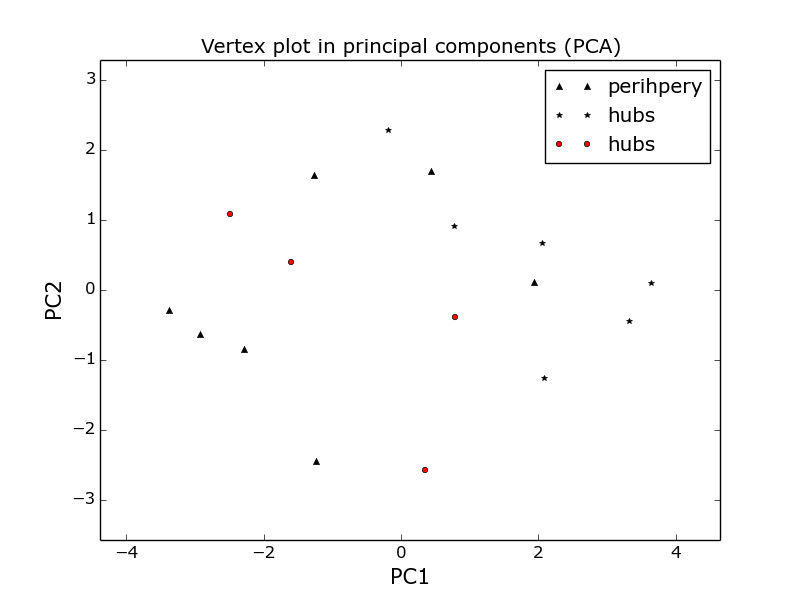
\includegraphics[width=0.3\textwidth]{figs/plot_pca}
%\label{fig:formation}
% \end{figure}
Principal components formation of textual and topological metrics
seems to be the less stable of all results reported in this study.
The concentration of dispersion often peaked in the intermediary sector.
% Clustering coefficient was dominant in a principal component almost exclusively
% when the whole network was used for PCA, otherwise it combined more evenly with
% other measures.
% This reveals that clustering coefficient might be a more relevant feature for the complete network
% than for each separate sector.
Components are most often composed of topological or textual features.
Other than that, we observe that PCA is sensitive to metrics included
and should reveal other insights in other settings.
These results are exemplified in Table~\ref{tab:tpca}.
\begin{table}[h!]
\begin{center}
\caption{PCA formation TAG: 11}
	\label{tab:tpca}
\begin{tabular}{| l || c | c | c | c | c |}\hline
 & {\bf PC1} & {\bf PC2} & {\bf PC3} & {\bf PC4} & {\bf PC5} \\\hline\hline
{\bf $cc$} & 1.56 & 5.55 & 5.27 & 66.36 & 4.43 \\
{\bf (p.)} & 2.07 & 21.29 & -3.09 & -16.58 & -30.47 \\
{\bf (i.)} & 3.53 & -5.95 & -6.72 & 51.70 & 8.40 \\
{\bf (h.)} & 9.65 & -14.73 & 3.26 & 14.54 & 27.15 \\\hline
{\bf $d$} & 3.28 & 39.23 & -2.42 & -3.75 & 1.71 \\
{\bf } & 2.31 & 29.69 & -4.90 & 7.49 & 10.16 \\
{\bf } & 6.23 & 18.94 & 16.55 & 7.89 & -1.65 \\
{\bf } & -10.34 & 13.75 & -14.11 & 5.08 & 9.43 \\\hline
{\bf $s$} & 2.89 & 39.14 & -2.73 & -6.53 & 2.19 \\
{\bf } & 2.30 & 29.95 & -4.12 & 6.71 & 9.55 \\
 & 6.37  & 19.06  & 16.00  & 10.14  & -1.42 \\
 & -9.80  & 13.47  & -14.84  & 6.58  & 13.35 \\\hline
$\mu_S(p)$ & 11.87  & -6.88  & -23.79  & 0.56  & 19.99 \\
 & -12.99  & -3.75  & -21.38  & 18.20  & -12.48 \\
 & 8.32  & -18.13  & 13.89  & 6.33  & -6.38 \\
 & 10.80  & -6.99  & -19.67  & 0.26  & 6.55 \\\hline
$\sigma_S(p)$ & 11.31  & -0.30  & -25.29  & 10.55  & -14.13 \\
 & -10.90  & -0.79  & -27.98  & -9.77  & 8.49 \\
 & 10.21  & -14.05  & 15.44  & -6.84  & 12.95 \\
 & 8.72  & -6.76  & -21.47  & 2.17  & -16.46 \\\hline
$\mu_S(kw)$ & 19.19  & -6.59  & -2.36  & -5.99  & 11.85 \\
 & -19.64  & 0.08  & -0.64  & 7.86  & -7.62 \\
 & 17.95  & -8.73  & 0.93  & -2.42  & -16.55 \\
 & 14.15  & 7.50  & -7.33  & -20.52  & 6.85 \\\hline
$\sigma_S(kw)$ & 17.26  & -1.70  & 1.16  & 0.48  & -24.22 \\
 & -17.26  & 1.60  & -1.20  & -18.84  & 10.50 \\
 & 16.92  & 2.12  & -4.56  & -13.03  & 22.97 \\
 & 13.31  & 10.62  & -1.67  & 19.42  & -11.12 \\\hline
$\mu_S(sw)$ & 15.36  & -0.55  & 19.90  & -4.40  & 14.27 \\
 & -14.96  & 6.19  & 21.48  & 9.07  & -5.17 \\
 & 15.77  & 4.76  & -12.12  & 0.29  & -20.25 \\
 & 12.34  & 12.79  & 7.28  & -15.30  & 8.15 \\\hline
$\sigma_S(sw)$ & 17.31  & -0.06  & 17.07  & -1.37  & -7.20 \\
 & -17.57  & 6.65  & 15.22  & -5.48  & 5.55 \\
 & 14.70  & 8.27  & -13.80  & -1.36  & 9.42 \\
 & 10.89  & 13.38  & 10.37  & 16.12  & -0.94 \\\hline\hline
$\lambda$ & 36.91  & 22.07  & 16.02  & 11.02  & 7.75 \\
 & 37.77  & 25.85  & 14.81  & 8.29  & 7.11 \\
 & 33.74  & 23.23  & 20.12  & 10.67  & 6.77 \\
 & 40.07  & 27.24  & 20.10  & 6.53  & 3.68 \\\hline
\end{tabular}
\begin{flushleft}
		Source: By the author.\
\end{flushleft}
\end{center}
\end{table}


\subsection{Results still to be interpreted}\label{subsec:sii}
%These networks yield diverse characteristics,
%some of which were not of core importance for this step of the research.
%Even so, at least one of these characteristics was found interesting enough to be considered a result and an example of interesting artifacts found.
Histogram differences of incident word sizes with and without repetition of words are constant.
That is, in each email list, when a histogram of word sizes was made with all words written, and another histogram made with sizes of all \emph{different} words, the cumulative absolute difference of the two histograms throughout the bins was found constant for all lists analysed.
When all known English words were considered, 
the difference sums up to $\approx 1.0$.
When stopwords are discarded,
the difference found was different, but still constant, slightly above $0.5$.
When only stopwords were considered, the difference is $\approx 0.6$.
When only known English words that do not have Wordnet synsets are used,
this difference is $\approx 1.2$.
We considered this result a number of times in the past years and presented it to other researchers,
but reached no conclusions about its meaning.
The ending figures of~\cite{textTables} are dedicated to these histogram differences.

\section{Results from visualization}\label{sec:versinus1}
The results associated with Versinus are divided into two groups:
observations on features that made it useful for the task of analyzing the general properties of human interaction networks,
and the network properties it made possible to grasp.

\subsection{Useful visualization features for dynamic networks}

Among the numerous insights related to Versinus, a few seem more fundamental, while others were simply useful. These
insights were incorporated to Versinus as the result of tests which presented clear benefits within the context of our research.
The following list is an attempt to present the observations and insights in an importance-first order:
\begin{enumerate}
\item Vertices need to remain static.
Even if they move smoothly, one should notice solely transient artifacts from the structure.
\item Very connected sectors (hubs and intermediary) need to be in a curve, otherwise the edges enclose each other and it is difficult to infer information from the network.
\item The height and width of a vertex are very informative, especially if metrics mapped to them have a strong relation, such as out-degree (mapped to height in Versinus) and in-degree (mapped to width).
\item The color of nodes is also informative although less than height and weight, as differences in the latter are more noticeable.
\item An ordering of nodes, related to their fixed position, is very useful. Among all tests, ordering of vertices by degree was considered the most informative, which led to the hub, intermediary and peripheral sectioning of the network delineated in Section~\ref{sectioning}.
As node position in the layout is fixed throughout an animation which comprises consecutive but distinct network activity, such ordering is done with respect to the resulting network of all the activity.
Numbering these positions with respect to the order of the vertices in the larger structure (i.e. all $M$ messages) is useful for understanding to which extent a vertex preserves the position in different scales of activity.
\end{enumerate}
Many other insights were derived from Versinus, such as possible visualization tools, other kinds of convenient layouts and glyph elaborations.
These received attention in Section~\ref{sec:verref}.

\subsection{Understanding of network properties through Versinus}\label{sec:enVer}
A number of hypotheses were drawn about the networks for which Versinus was designed.
As suggested by Palla, Barab\'asi and Vicsek~\cite{barabasiEvo}, stability of participant activity in social networks is more incident in smaller networks.
Consistent with this result, all hubs have intermittent activity in the settings analyzed, except for the email list with the smallest number of participants (the Metareciclagem email list).
The intermittence of hubs was one of the top hypotheses which motivated the development of Versinus.
The stability of the network structure, concomitant with the instability of the activity of each participant,
motivated a deeper analysis~\cite{stab}.
In doing so, we also found evidence for another hypothesis drawn from Versinus:
that in- and out-degree differences in each vertex are important for network characterization.
Furthermore, the visualization suggests that there are modes of operation of the network.
As an example, the intermediary sector often communicates mostly with the hubs or with the peripheral vertices.
Other hypotheses,
such as discrepancies in the authority and the degree of a vertex,
are numerous but need further research to be validated.

\subsection{Mapping of network features to musical audio}\label{sec:veraud}
The later implementations of Versinus included sound
which was in sync with the animation.
These audio tracks were a enrichment to the visualizations
but were not fundamental for our understanding of the network structures
mainly because the measurements to which the sounds related were better
grasped by the visual clues.
The main implementation of these mappings of topology to musical sounds
can be summarized as follows:
\begin{itemize}
	\item The degree of the four most connected agents (considering the network with all the messages used for the animation) was used.
	\item Three audio signals (``voices'' in music jargon) were made: one with a bandwidth restricted brown noise and two with defined pitch.
	\item The measures from the two most connected agents were mapped to the bandwidth and central frequency of the brown noise.
	\item The measures from the third and fourth most connected agents were mapped to the pitch of the pitch defined voices.
	\item The sound characteristics were updated in durations that were multiples of a pulse, resulting in a well-marked rhythm.
	\item The voices with defined pitch could be set to have more than one note with the same pitch before updating the pitch.
\end{itemize}

This procedure resulted in the ``Four Hubs Dance''~\cite{animacoes}.
It might be noteworthy that data exploration through sounds is still very incipient
in the scientific literature and that this musical mapping of dynamic networks features
is potentially singular.
The dissertation~\cite{mad} is handy in understanding the synthesis of these highly precise mappings
and for enhancements.


\subsection{Refinement of Versinus}\label{sec:verref}
Versinus was convenient for obtaining insights about how to enhance its layout and use.
It was immediate to think of a tool for using Versinus
in real-time, but less obvious are some ideas about the layout and visual guides. 
To further enable visualization of hubs and intermediary vertex,
the sinusoid can have many periods 
with a decaying frequency.
The upper straight line can also have an oscillating outline.
The two halves of the sinusoidal period could be moved independently.
The waveform need not to be a sinusoid.
One can think of many ways to make more informative glyphs.
Also, visual and auditory signals for specific occurrences can be interesting
(e.g. when a new vertex appears, when one vanishes, when an ordering of vertices changes).
Measurements of each vertex can be shown with a vertical displacement,
to enable multiple measurements, to avoid the need to blink the numbers and to keep network visualization free from occlusion.
Working with Versinus has also suggested other kinds of layouts for vertices, 
especially geometric figures and iterative force-based methods for positioning vertices in a fixed layout.
The traditional matrix representation of the graphs has been gazed upon as support to Versinus 
as has been some recent approaches to network visualization~\cite{Viz1}.


\section{Linked data results}
\label{outline}
The current results include data selection and preparation for knowledge discovery.
In this respect, the main result lies in the fact that data were made available, which enables benchmarking of scientific results
and experimentations.
Secondary results include data outline through figures and tables,
software support and example SparQL queries.

\subsection{Standardization}
The data is embedded into standard URIs and triples, i.e. translated to RDF.
URIs are built in the namespace \url{http://purl.org/socialparticipation/participationontology/}
which are identified herein with the prefix \textttt{po:}.
Classes and properties are built by adding a suffix to the root,
as in the class \textttt{po:Participant} or in the property \textttt{po:text}.
Classes have ``UpperCamelCase'' suffixes while properties have ``lowerCamelCase'' suffixes.
All class instances, such as participants, messages, friendships and
interactions, are linked to
snapshots through the triple \textttt{<instance> po:snapshot <snapshot\_uri>}.
Message texts, including comments, are objects in the triple: \textttt{<message\_id> po:text <message\_text>}.
Preprocessed texts are objects of triples: \textttt{<message\_id> po:cleanText <message\_text>}.
More specialized predicates are used for delivering text when necessary,
such as \textttt{po:htmlBodyText} and \textttt{po:cleanBodyText} used
for ParticipaBR articles (instances of the class \textttt{po:Article}.
A participant URI is unique throughout the provenance (e.g. the same for
the same participant in all Twitter snapshots).
To enable annotations which differ when the snapshot changes,
\textttt{po:Observation} class instances are used in the triple
\textttt{<participant\_uri> po:observation <observation\_uri>}.
The observation instances are then linked to the snapshot and the
data.



Instances are built on top of the class they derive from plus a hashtag character,
a provenance string (e.g. \textttt{facebook-legacy} or
\textttt{participabr-legacy}) of the snapshot they refer to, and an identifier;
i.e. \textttt{po:Participant\#<provenance-legacy>-<id>}.
All snapshot URIs follow the formation rule: \textttt{po:<SnapshotProvenance>\#<snapshot\_id>}.
All snapshot ids follow the formation rule: \textttt{<platform>-legacy-<further\_identifier>}; e.g.
\textttt{irc-legacy-labmacambira} or
\textttt{email-legacy-linux.audio.devel1-20000}.
\subsection{Data outline}
The database consists of 34,120,026 triples, 3,172,927 edges yield by interactions or relations, 382,568 participants and 253,155,020 characters. Among all snapshots, 63 are ego snapshots, 54 are group snapshots; 49 have interaction edges, 89 have friendship edges; 43 have text content from messages.

\begin{table*}[h!]
\begin{center}
\caption{Number of snapshots from each provenance.}
\begin{tabular}{| l | c |}\hline
\textbf{social protocol} & \textbf{number of snapshots} \\\hline\hline
Algorithmic Autoregulation & 3 \\\hline
Cidade Democrática & 1 \\\hline
Email & 4 \\\hline
Facebook & 88 \\\hline
IRC & 4 \\\hline
ParticipaBR & 1 \\\hline
Twitter & 16 \\\hline\hline
all & 117 \\\hline
\end{tabular}\end{center}
\end{table*}
% stats:
%% number of triples
%% number of edges
%% number of chars
%% number of users
% diagrams in the supporting information file
\subsection{Software tools}
The database is released with software for rendering itself, analyses and
multimedia artifacts.
\subsubsection{Triplification routines}
For each social platform there is a \emph{triplification} routine,
i.e. a script for translating data to RDF.
Original formats and further observations are presented in
Table~\ref{tab:provenance}.
\begin{table*}[h!]\scriptsize
\begin{center}
\caption{Social platforms, original formats and further observations for
the database.}\label{tab:provenance}
	\def\arraystretch{1.2}
\begin{tabular}{l || p{3cm} | p{3cm} | c}\hline
\textbf{social platform} & \textbf{original format} & \textbf{further observations} & \textbf{toolbox} \\\hline\hline
AA & MySQL and MongoDB databases; IRC text logs & donated by AA users & Participation~\cite{participation} \\\hline
Cidade Democrática & MySQL database & donated by admins & Participation \\\hline
Email & mbox & obtained through Gmane public database & Gmane~\cite{gmane} \\\hline
Facebook & GDF, GML and TAB & obtained through Netvizz~\cite{netvizz} & Social~\cite{fbtwData} \\\hline
IRC & plain text log & obtained through Supybot logging & Social \\\hline
ParticipaBR & PostgreSQL database & donated by admins & Participation \\\hline
Twitter & JSON & obtained through Twitter streaming API & Social \\\hline
\end{tabular}
\begin{flushleft}\footnotesize
Source: By the author.\
\end{flushleft}
\end{center}
\end{table*} 


\subsubsection{Topological and textual analysis}\label{ana}
Routines are available for taking the topological and textual measurements from
the database.
Auxiliary routines, such as performing principal component analysis
and taking Kolmogorov-Smirnov measurements, are available
to facilitate pattern recognition.
All the analysis routines used for this thesis are in these publicly accessible scripts.

\subsubsection{Multimedia rendering}\label{media}
It is a core purpose of the framework to provide routines for rendering
audiovisualizations of the data.
Social structures are rendered into music, images and video animations
through the Percolation toolbox~\cite{gmanePack} in association with
the Music and Visuals toolboxes~\cite{music,visuals}.

\subsubsection{Migration from deprecated toolboxes}
Routines mentioned in Sections~\ref{ana} and~\ref{media} are being migrated from deprecated
toolboxes~\cite{gmaneLegacy,percolationLegacy} into newly designed
toolboxes~\cite{gmaneLegacy,percolationLegacy} into newly designed
toolboxes~\cite{gmanePack,visuals}.

\subsection{Diagrams of the data and auxiliary tables}
The database exploration can be assisted through diagrams which shows
the structure from each provenance.
Such diagrams are
are fully available in an article~\cite{losd}
with some tables to make it easier to understand the data provided.
A simplified example is given in Figure~\ref{dia} where the friendship
structure of the Facebook snapshots is illustrated.

\begin{figure}[!ht]
\centering
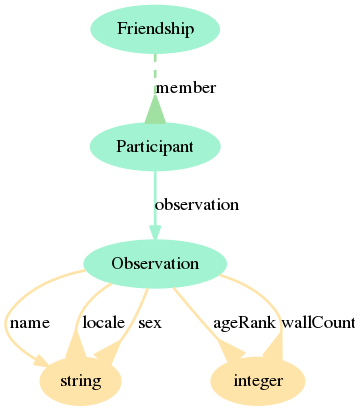
\includegraphics[width=0.5\textwidth]{ontologies/facebook-legacy-AntonioAnzoategui18022013Friendship.ttl/draw}
\caption{A diagram of the structure involved in the friendship networks
of the Facebook snapshots.
A green edge denotes an OWL existential class restriction;
an inverted nip denotes an OWL universal class restriction;
a full (non-dashed) edge denotes an OWL functional property axiom.
Further information and complete diagrams for each provenance are given in ~\cite{losd}.}\label{dia}
\begin{flushleft}\footnotesize
Source: By the author.\
\end{flushleft}
\end{figure}


\subsection{SPARQL queries}\label{queries}
There are numerous useful and general purpose SPARQL queries to be performed against the database.
Here we write some of such queries selected by their simplicity and potential to be varied.
All queries assume the use of the preamble \textttt{PREFIX po: <http://purl.org/socialparticipation/po/>}.
\begin{enumerate}[leftmargin=0cm]
\item Retrieve the number of participants:\\
\textttt{SELECT (COUNT(DISTINCT ?author) as ?c) WHERE \{
?author a po:Participant . \} }
\item Retrieve the number of relations, be them interactions or
friendships:\\
\textttt{SELECT (COUNT(?interaction) as ?c) WHERE \{\\
\h \{ ?interaction a po:Friendship \} UNION \{ ?interaction
a po:Interaction \} UNION\\
\h \{ ?interaction po:retweetOf
?message \} UNION \{ ?interaction po:replyTo ?message
\}\\
\h UNION \{ ?interaction po:directedTo ?participant
\}\\ \} }
\item Retrieve all text produced by a specific user:\\
\textttt{SELECT (CONCAT(?text) as ?texts) WHERE \{\\
\h ?activity po:author <user\_uri> . ?activity po:text ?text .\\
\}}
\item List 1000 users (URIs and names) with the most friendships and the number of
friendships in descending order by the number of friendships:\\
\textttt{SELECT DISTINCT ?participant (COUNT(?friendship)
as ?c) WHERE \{\\
\h ?friendship a po:Friendship . ?friendship po:member ?participant . \\
\} ORDER BY DESC(?c) LIMIT 1000}
\item Retrieve text messages with the word ``pineapple'' (case insensitive):\\
\textttt{SELECT ?text WHERE \{ \\
\h ?activity po:text ?text . FILTER regex(?text, 'pineapple', 'i')\\
\}}
\item List participants and respective full names whose name has the substring ``Amanda'':\\
\textttt{SELECT DISTINCT ?participant ?name WHERE \{\\
\h ?participant po:observation ?obs . ?obs po:name ?name .\\
\h FILTER regex(?name, 'Amanda', 'i') \\
\}}
\item Return all pairs of friends of a participant which are friends themselves:\\
\textttt{SELECT DISTINCT ?friend1 ?friend2 WHERE \{\\
\h ?friendship1 po:member <participant\_uri> . ?friendship1 po:member ?friend1 .\\
\h ?friendship2 po:member <participant\_uri> . ?friendship2 po:member ?friend2 .\\
\h ?friendship3 po:member ?friend1 . ?friendship3 po:member ?friend2 .\\
\}}
\item Return all interactions from replies in a snapshot:\\
\textttt{SELECT ?from ?to WHERE \{\\
\h ?message1 po:snapshot <snapshot\_uri> . ?message2 po:replyTo ?message1 .\\
\h ?message1 po:author ?from . ?message2 po:author ?to .\\
\}}
\end{enumerate}

\subsection{License issues}
% Facebook, Twitter, IRC, Gmane, Participa, CD, AA.
The database presented in this thesis is released under public domain.
Computer scripts are in git repositories and PyPI Python packages, also under public domain.
Although most data is already in open licenses (Twitter, Email, Participabr, Cidade Democrática, and AA data), IRC and Facebook data was collected
and donated by the individuals which yielded the data.
This rises the understanding of the right to study such data as the right to access the self,
in line with anthropological endeavors~\cite{anPhy,antphy2}.


\subsection{Data-driven ontology synthesis}\label{sec:ontSyn}
OWL Ontologies are critical tools to describe taxonomies and the
structure of knowledge.
Most ontologies are created by domain experts even though there often is data they
organize that is given by a software system and which has a predefined
structure. 

We developed a simple ontology synthesis method that probes
the ontological structure in data with
SPARQL queries and post-processing.
The results are OWL code and diagrams which are 
available in an article~\cite{losd}.
The method can be extended to comprise further OWL axioms and restrictions,
but is currently performed to fit present needs with maximum simplicity.
The present needs are limited to informative figures and
the steps implemented are as follows:
\begin{enumerate}[leftmargin=0cm]
\item Obtain all distinct classes with the query:\\
\textttt{SELECT DISTINCT ?class\_uri WHERE \{ ?s a ?class\_uri \}}
\item For each class, obtain the properties that occur as predicates in triples where the subject is an instance of the class:\\
\textttt{SELECT DISTINCT ?property\_uri WHERE \{ ?s a <class\_uri> . ?s ?property\_uri ?o . \}}\\
Such properties are used to assert existential and universal restrictions for the class.
\item Compare the total number of individuals (\textttt{?cs1}) of the class (\textttt{class\_uri}) with
the number of such individuals (\textttt{?cs2}) that are subjects of at least one triple where 
the predicate is the property (\textttt{property\_uri}).
If the numbers match, there is an existential restriction for the class. The queries are:\\
\textttt{SELECT (COUNT(DISTINCT ?s) as ?cs1) WHERE \{ ?s a <class\_uri> \}}\\
\textttt{SELECT (COUNT(DISTINCT ?s) as ?cs) WHERE \{\\
\h ?s a <class\_uri>. ?s <property\_uri> ?o .\\ \}}
\item Find the number of instances which are subjects of triples where the predicate is the property but are not instances of the class.
If there is zero of such instances, there is a universal restriction:\\
\textttt{SELECT (COUNT(DISTINCT ?s)=0 as ?cs) WHERE \{\\
\h ?s <property\_uri> ?o . ?s a ?ca . FILTER(str(?ca) != 'class\_uri')\\ \}}
\item To keep a record of the restrictions (and occurring triples), get all object classes or datatypes where the subject is an instance of the class and the predicate is the property:\\
\textttt{SELECT DISTINCT ?co (datatype(?o) as ?do) WHERE \{\\
\h ?s a <class\_uri>. ?s <property\_uri> ?o . OPTIONAL \{ ?o a ?co . \}\\
\}}
\item Obtain all distinct properties:\\
\textttt{SELECT DISTINCT ?p WHERE \{ ?s ?p ?o \}}
\item Check if each property is functional, i.e. if it
occurs at most once with each subject.
This is performed by counting the objects and further verifying
that they are at most one. The query is:\\
\textttt{SELECT DISTINCT (COUNT(?o) as ?co) WHERE \{ ?s
<property\_uri> ?o \} GROUP BY ?s}
\item For each property, find the incident range and domain with the
queries:\\
\textttt{SELECT DISTINCT ?co (datatype(?o) as ?do) WHERE \{\\
\h ?s <property\_uri> ?o . OPTIONAL \{ ?o a ?co . \}\\\}} \\
and \\
\textttt{SELECT DISTINCT ?cs WHERE \{ ?s <property\_uri> ?o . ?s a ?cs . \}}
\item Render diagrams as explained in the next section and in~\cite{losd}.
\end{enumerate}



% ---
% Capítulo 4
% ---
%% USPSC-Cap3-Conclusao.tex
% Capítulo 3 - Conclusão
% ---
% Conclusão
% ---
\chapter{Conclusion and Future Work}
% ---
% O comando abaixo insere parágrafos aleatórios só para exemplificar
Apresentar as conclusões correspondentes aos objetivos ou hipóteses propostos para o desenvolvimento do trabalho, podendo incluir  sugestões para novas pesquisas.

O Grupo desenvolvedor do Pacote USPSC, atualmente composto da Classe USPSC e do  Modelo para teses e dissertações em \LaTeX\ utilizando a classe USPSC, acredita que esta ferramenta propiciará o aprimoramento na qualidade dos trabalhos acadêmicos produzidos pelos alunos de pós-graduação das Unidades de Ensino e Pesquisa do Campus USP de São Carlos, garantindo a normalização e padronização estabelecidas.

Já está sendo elaborado o Modelo para Trabalhos de Conclusão de Cursos em \LaTeX\ utilizando a classe USPSC em conformidade com  a \textbf{ABNT NBR 14724}: informação e documentação: trabalhos acadêmicos: apresentação \cite{nbr14724}, \textbf{Diretrizes para apresentação de dissertações e teses da USP}: documento eletrônico e impresso - Parte I (ABNT) \cite{sibi2009} e normas e padrões estabelecidos pelas Unidades.

O Grupo desenvolvedor do Pacote USPSC já está trabalhando para que a Classe USPSC seja uma  customização em conformidade com as orientações dadas em \url{https://github.com/abntex/abntex2/wiki/ComoCustomizar}.

A expectativa é de que tais soluções sejam adotadas por outras Unidades da USP e outras instituições interessadas, sendo que a facilidade de customização fatalmente contribuirá para tanto.




% ---

% Capítulo 5 - Conclusão
% ---
% \include{USPSC-Cap5-Conclusao}
% ---

% ----------------------------------------------------------
% ELEMENTOS PÓS-TEXTUAIS
% ----------------------------------------------------------
\postextual
% ----------------------------------------------------------

% -----------------------------------------------------------
% Referências bibliográficas
% ----------------------------------------------------------
\bibliography{USPSC-modelo-references}

% ----------------------------------------------------------
\newpage~
% Glossário
% ----------------------------------------------------------
%
% Consulte o manual da classe abntex2 para orientações sobre o glossário.
%
%\glossary

% ----------------------------------------------------------
% Apêndices
% ----------------------------------------------------------
%% USPSC-Apendice.tex
% ---
% Inicia os apêndices
% ---

\begin{apendicesenv}
	% Imprime uma página indicando o início dos apêndices
	\partapendices
	\chapter{Additional tables of the textual differences found in all networks}\label{ap:textd}
In the following tables the counting of differences of textual features among the analyzed networks
are shown.
	These results are auxiliary for the discussion on Section~\ref{sec:tresults}.
\FloatBarrier
\begin{table}[h!]
\begin{center}
\caption{Counts of evidence of characters-related differences in the Erd\"os sectors in each of the analyzed networks.}
	\def\arraystretch{1.5}
\begin{tabular}{| l || c | c | c || c |}\hline
{\bf synset} & {\bf p.} & {\bf i.} & {\bf h} & {\bf peaks} \\\hline\hline
$\frac{spaces}{chars}$ & 2  & 0  & 8  & 2 \\
$\frac{punct}{chars-spaces}$ & 11  & 4  & 1  & 5 \\
$\frac{digits}{chars-spaces}$ & 9  & 7  & 2  & 10 \\\hline
$\frac{letters}{chars-spaces}$ & 0  & 0  & 3  & 0 \\
$\frac{vowels}{letters}$ & 0  & 1  & 1  & 1 \\
$\frac{uppercase}{letters}$ & 13  & 3  & 1  & 6 \\\hline
\end{tabular}
\begin{flushleft}
		Source: By the author.\
\end{flushleft}
\end{center}
\end{table}

\begin{table}[h!]
\begin{center}
\caption{Counts of evidence of token-related differences in the Erd\"os sectors in each of the analyzed networks.}
	\def\arraystretch{1.5}
\begin{tabular}{| l || c | c | c || c |}\hline
{\bf synset} & {\bf p.} & {\bf i.} & {\bf h} & {\bf peaks} \\\hline\hline
$\frac{knownw}{tokens}$ & 1  & 0  & 5  & 1 \\
$\frac{knownw \neq}{knownw}$ & 13  & 1  & 4  & 9 \\
$\frac{stopw}{knownw}$ & 0  & 0  & 14  & 2 \\
$\frac{punct}{tokens}$ & 10  & 3  & 1  & 3 \\
$\frac{contrac}{tokens}$ & 0  & 2  & 15  & 4 \\\hline
$\mu(\overline{tokens})$ & 0  & 1  & 2  & 1 \\
$\sigma(\overline{tokens})$ & 7  & 1  & 0  & 2 \\\hline
$\mu(\overline{knownw})$ & 0  & 0  & 2  & 0 \\
$\sigma(\overline{knownw})$ & 0  & 0  & 1  & 1 \\\hline
$\mu(\overline{knownw \neq})$ & 0  & 0  & 0  & 0 \\
$\sigma(\overline{knownw \neq})$ & 0  & 0  & 0  & 0 \\\hline
$\mu(\overline{stopw})$ & 0  & 0  & 0  & 0 \\
$\sigma(\overline{stopw})$ & 0  & 0  & 1  & 0 \\\hline
\end{tabular}
\begin{flushleft}
		Source: By the author.\
\end{flushleft}
\end{center}
\end{table}

\begin{table}[h!]
\begin{center}
\caption{Counts of evidence of sentence-related differences in the Erd\"os sectors in each of the analyzed networks.}
\begin{tabular}{| l || c | c | c || c |}\hline
{\bf synset} & {\bf p.} & {\bf i.} & {\bf h} & {\bf peaks} \\\hline\hline
$\mu_S(chars)$ & 9  & 3  & 1  & 6 \\
$\sigma_S(chars)$ & 11  & 6  & 1  & 9 \\\hline
$\mu_S(tokens)$ & 10  & 2  & 1  & 5 \\
$\sigma_S(tokens)$ & 9  & 7  & 1  & 9 \\\hline
$\mu_S(knownw)$ & 9  & 3  & 2  & 6 \\
$\sigma_S(knownw)$ & 11  & 5  & 2  & 8 \\\hline
$\mu_S(stopw)$ & 2  & 3  & 7  & 7 \\
$\sigma_S(stopw)$ & 6  & 7  & 4  & 10 \\\hline
$\mu_S(puncts)$ & 13  & 2  & 1  & 2 \\
$\sigma_S(puncts)$ & 7  & 8  & 1  & 8 \\\hline
\end{tabular}
\begin{flushleft}
		Source: Prepared by the authors.\
\end{flushleft}
\end{center}
\end{table}

\begin{table}[h!]
\begin{center}
\caption{Counts of evidence of message-related differences in the Erd\"os sectors in each of the analyzed networks.}
	\def\arraystretch{1.5}
\begin{tabular}{| l || c | c | c || c | c |}\hline
{\bf synset} & {\bf p.} & {\bf i.} & {\bf h} & {\bf peaks} & {\bf total} \\\hline\hline
$\mu_M(sents)$ & 4  & 7  & 1  & 9  & 16 \\
$\sigma_M(sents)$ & 5  & 7  & 2  & 11  & 15 \\\hline
$\mu_M(tokens)$ & 10  & 5  & 2  & 6  & 18 \\
$\sigma_M(tokens)$ & 8  & 8  & 2  & 9  & 18 \\\hline
$\mu_M(knownw)$ & 8  & 5  & 3  & 7  & 18 \\
$\sigma_M(knownw)$ & 10  & 5  & 3  & 9  & 18 \\\hline
$\mu_M(stopw)$ & 5  & 6  & 6  & 8  & 18 \\
$\sigma_M(stopw)$ & 7  & 6  & 3  & 11  & 18 \\\hline
$\mu_M(puncts)$ & 12  & 4  & 2  & 5  & 18 \\
$\sigma_M(puncts)$ & 8  & 9  & 1  & 10  & 18 \\\hline
$\mu_M(chars)$ & 10  & 5  & 2  & 6  & 18 \\
$\sigma_M(chars)$ & 9  & 7  & 2  & 8  & 18 \\\hline
\end{tabular}
\begin{flushleft}
		Source: Prepared by the authors.\
\end{flushleft}
\end{center}
\end{table}

\begin{table}[h!]
\begin{center}
\caption{Counts of evidence of differences related to POS tags in the Erd\"os sectors in each of the analyzed networks.}
\begin{tabular}{| l || c | c | c || c |}\hline
{\bf synset} & {\bf p.} & {\bf i.} & {\bf h} & {\bf peaks} \\\hline\hline
NOUN & 13  & 1  & 0  & 1 \\
X & 4  & 9  & 5  & 14 \\\hline
ADP & 0  & 1  & 4  & 1 \\
DET & 1  & 0  & 9  & 2 \\\hline
VERB & 0  & 0  & 6  & 1 \\\hline
ADJ & 1  & 2  & 6  & 2 \\
ADV & 0  & 0  & 17  & 1 \\\hline
PRT & 1  & 1  & 9  & 4 \\
PRON & 0  & 1  & 11  & 3 \\
NUM & 8  & 5  & 3  & 7 \\
CONJ & 2  & 6  & 4  & 8 \\\hline
\end{tabular}
\begin{flushleft}
		Source: By the author.\
\end{flushleft}
\end{center}
\end{table}

\begin{table}[h!]
\begin{center}
\caption{Counts of evidence of differences related to Wordnet POS tags in the Erd\"os sectors in each of the analyzed networks.}
\begin{tabular}{l || c | c | c || c}\hline
{\bf synset} & {\bf p.} & {\bf i.} & {\bf h} & {\bf peaks} \\\hline\hline
N & 8  & 1  & 0  & 1 \\
ADJ & 0  & 2  & 12  & 6 \\
VERB & 0  & 1  & 16  & 2 \\
ADV & 0  & 0  & 9  & 1 \\\hline\hline
POS & 0  & 0  & 3  & 1 \\
POS! & 0  & 1  & 0  & 1 \\\hline
\end{tabular}
\begin{flushleft}\footnotesize
		Source: By the author.\
\end{flushleft}
\end{center}
\end{table}

\begin{table}[h!]
\begin{center}
\caption{Counts of evidence of differences related to Wordnet noun synset characteristics in the Erd\"os sectors in each of the analyzed networks.}
\begin{tabular}{| l || c | c | c || c |}\hline
{\bf synset} & {\bf p.} & {\bf i.} & {\bf h} & {\bf peaks} \\\hline\hline
$\mu(min\,depth)$ & 0  & 0  & 0  & 0 \\
$\sigma(min\,depth)$ & 1  & 1  & 2  & 1 \\\hline
$\mu(max\,depth)$ & 0  & 0  & 0  & 0 \\
$\sigma(max\,depth)$ & 0  & 1  & 3  & 1 \\\hline
$\mu(holonyms)$ & 7  & 4  & 4  & 6 \\
$\sigma(holonyms)$ & 3  & 4  & 7  & 6 \\\hline
$\mu(meronyms)$ & 8  & 5  & 3  & 7 \\
$\sigma(meronyms)$ & 12  & 4  & 2  & 9 \\\hline
$\mu(domains)$ & 6  & 4  & 5  & 8 \\
$\sigma(domains)$ & 3  & 1  & 4  & 3 \\\hline
$\mu(lemmas)$ & 6  & 0  & 1  & 2 \\
$\sigma(lemmas)$ & 6  & 2  & 2  & 4 \\\hline
$\mu(hyponyms)$ & 1  & 6  & 6  & 9 \\
$\sigma(hyponyms)$ & 4  & 6  & 6  & 11 \\\hline
$\mu(hypernyms)$ & 0  & 0  & 0  & 0 \\
$\sigma(hypernyms)$ & 4  & 4  & 4  & 6 \\\hline
\end{tabular}
\begin{flushleft}
		Source: Prepared by the authors.\
\end{flushleft}
\end{center}
\end{table}

\begin{table}[h!]
\begin{center}
\caption{Counts of evidence of differences related to Wordnet adjective synset characteristics in the Erd\"os sectors in each of the analyzed networks.}
\begin{tabular}{| l || c | c | c || c |}\hline
{\bf synset} & {\bf p.} & {\bf i.} & {\bf h} & {\bf peaks} \\\hline\hline
$\mu(domains)$ & 2  & 6  & 8  & 10 \\
$\sigma(domains)$ & 2  & 4  & 5  & 7 \\\hline
$\mu(similar)$ & 1  & 0  & 7  & 4 \\
$\sigma(similar)$ & 4  & 0  & 5  & 3 \\\hline
$\mu(lemmas)$ & 1  & 2  & 1  & 2 \\
$\sigma(lemmas)$ & 6  & 3  & 4  & 6 \\\hline
\end{tabular}
\begin{flushleft}
		Source: By the author.\
\end{flushleft}
\end{center}
\end{table}

\begin{table}[h!]
\begin{center}
\caption{Counts of evidence of differences related to Wordnet verb synset characteristics in the Erd\"os sectors in each of the analyzed networks.}
\begin{tabular}{| l || c | c | c || c |}\hline
{\bf synset} & {\bf p.} & {\bf i.} & {\bf h} & {\bf peaks} \\\hline\hline
$\mu(min\,depth)$ & 2  & 1  & 1  & 3 \\
$\sigma(min\,depth)$ & 2  & 1  & 1  & 2 \\\hline
$\mu(max\,depth)$ & 2  & 1  & 0  & 1 \\
$\sigma(max\,depth)$ & 3  & 1  & 1  & 2 \\\hline
$\mu(domains)$ & 7  & 3  & 4  & 4 \\
$\sigma(domains)$ & 8  & 3  & 3  & 5 \\\hline
$\mu(verb\,groups)$ & 0  & 2  & 3  & 2 \\
$\sigma(verb\,groups)$ & 0  & 0  & 0  & 0 \\\hline
$\mu(lemmas)$ & 0  & 0  & 2  & 0 \\
$\sigma(lemmas)$ & 1  & 0  & 3  & 0 \\\hline
$\mu(entailments)$ & 7  & 1  & 7  & 3 \\
$\sigma(entailments)$ & 4  & 1  & 5  & 3 \\\hline
$\mu(hyponyms)$ & 1  & 2  & 6  & 3 \\
$\sigma(hyponyms)$ & 2  & 3  & 8  & 6 \\\hline
$\mu(hypernyms)$ & 2  & 2  & 0  & 2 \\
$\sigma(hypernyms)$ & 1  & 0  & 1  & 1 \\\hline
\end{tabular}
\begin{flushleft}
		Source: By the author.\
\end{flushleft}
\end{center}
\end{table}

\begin{table}[h!]
\begin{center}
\caption{Counts of evidence of differences related to Wordnet adverb synset characteristics in the Erd\"os sectors in each of the analyzed networks.}
\begin{tabular}{| l || c | c | c || c |}\hline
{\bf synset} & {\bf p.} & {\bf i.} & {\bf h} & {\bf peaks} \\\hline\hline
$\mu(domains)$ & 3  & 3  & 10  & 10 \\
$\sigma(domains)$ & 1  & 4  & 7  & 7 \\\hline
$\mu(lemmas)$ & 0  & 0  & 1  & 1 \\
$\sigma(lemmas)$ & 3  & 1  & 2  & 4 \\\hline
\end{tabular}
\begin{flushleft}
		Source: Prepared by the authors.\
\end{flushleft}
\end{center}
\end{table}


\chapter{Developments made in this research but not included elsewhere in this thesis}\label{ap:vot}
In this appendix are gathered developments relevant for the initial proposal of this research:
enabling the use of complex networks scientific knowledge by the participant of the social networks.
These developments are not included elsewhere in the thesis because we chose to present results
more closely related to physics in a simple fashion.
Furthermore, most of the following contributions have received dedicated documentation,
reason why we next only summarize and cite the documents when they are available.

\section{Continuous voting by approval and participation}
In finding the adequate way to prioritize proposals, the Brazilian social participation community agreed about the measurement of two indexes,
one of approval and one of participation. Both practice and literature
was constantly handled by the experts involved, and the formalization
of such model and metrics and is very simple and seems novel.
Also, the relevance of this development is strengthened by the use of these indexes by the
Brazilian General Secretariat of the Republic to raise and prioritize
proposals about public health care in open processes.
This was achieved by means of the Dialoga Brasil federal platform~\cite{dialoga}.
A short report on these indexes and their use is on~\cite{dialogaAlg}
	(co-authorship by Ricardo Poppi).

	\section{Visualization of static networks}
	In Sections~\ref{sec:versinus0} and~\ref{sec:versinus1} we addressed a visualization method of networks through animations.
	We also made many static network visualizations which were important for our research.
	Many of these were made by testing software and programming libraries.
	We next exemplify such efforts by probably the most important and time-consuming realizations.

	\subsection{Static email networks visualization using Networkx and Graphviz and a PHP web interface}\label{sec:autoRede}
	At the start of this research, we observed many networks derived from email lists
	by means of a web interface we wrote.
	In such web interface, which was accessed as a usual webpage through HTTP in a web browser, 
	the user could specify an email list, start and end messages and a window size (number of messages taken together to obtain the network).
	The interface then rendered graph visualizations and standard measures such as degree, strength, clustering coefficient, betweenness centrality, both as histograms and as mean and standard deviation.
	In the node-link diagrams, measurements were mapped to height, width and color of nodes and to link characteristics.
	The software source code is available in~\cite{autoRede} and an example image is Figure~\ref{fig:autoRede}.
\begin{figure}[h!]
\begin{center}
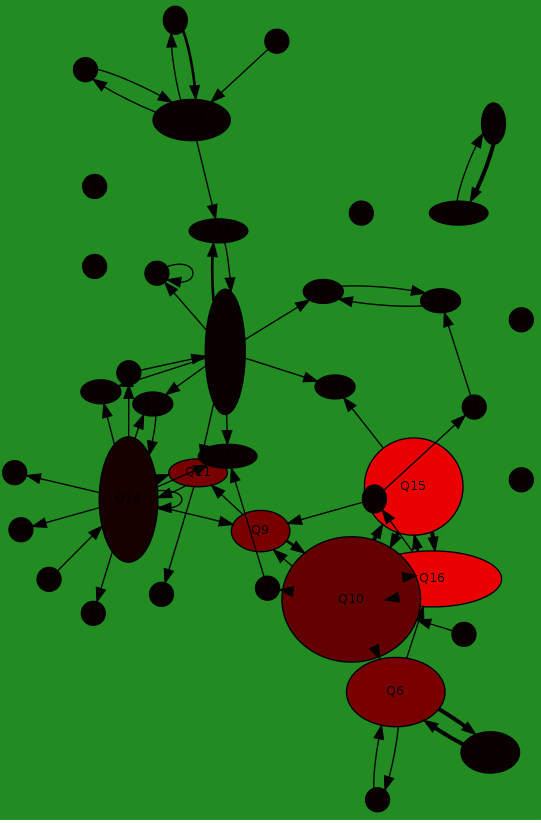
\includegraphics[scale=.25]{figs/autoRede_}
\caption{An example image rendered from the first online gadget made in this research for studying social networks.
	The app also delivered measurements, 2D plots and GML graph files. For further information please see Section~\ref{sec:autoRede}}
\label{fig:autoRede}
\begin{flushleft}\footnotesize
Source: By the author.\
\end{flushleft}
\end{center}
\end{figure}
% email pelo app online

	\subsection{Static Facebook networks visualization using Gephi}\label{sec:gephi}
	Mainly in the years of 2013 and 2014, Facebook users retrieved their friendship networks through Netvizz software~\cite{netvizz}
	and donated them to our research.
	I also retrieved friendship and interaction networks from Facebook groups I was a member, also using Netvizz.
	These networks were used for information collection and diffusion (explained in Section~\ref{sec:colDif}),
	taking measurements and visualization.
	The visualizations were achieved almost exclusively through the Gephi software~\cite{gephi}
	and is included in this appendix for being used a number of times by fellow researchers and artists.
	The most useful layout algorithm was Force Atlas 2~\cite{fa2} and an example of these images is Figure~\ref{fig:gephi}.

% \begin{figure}[h!]
% \begin{center}
% 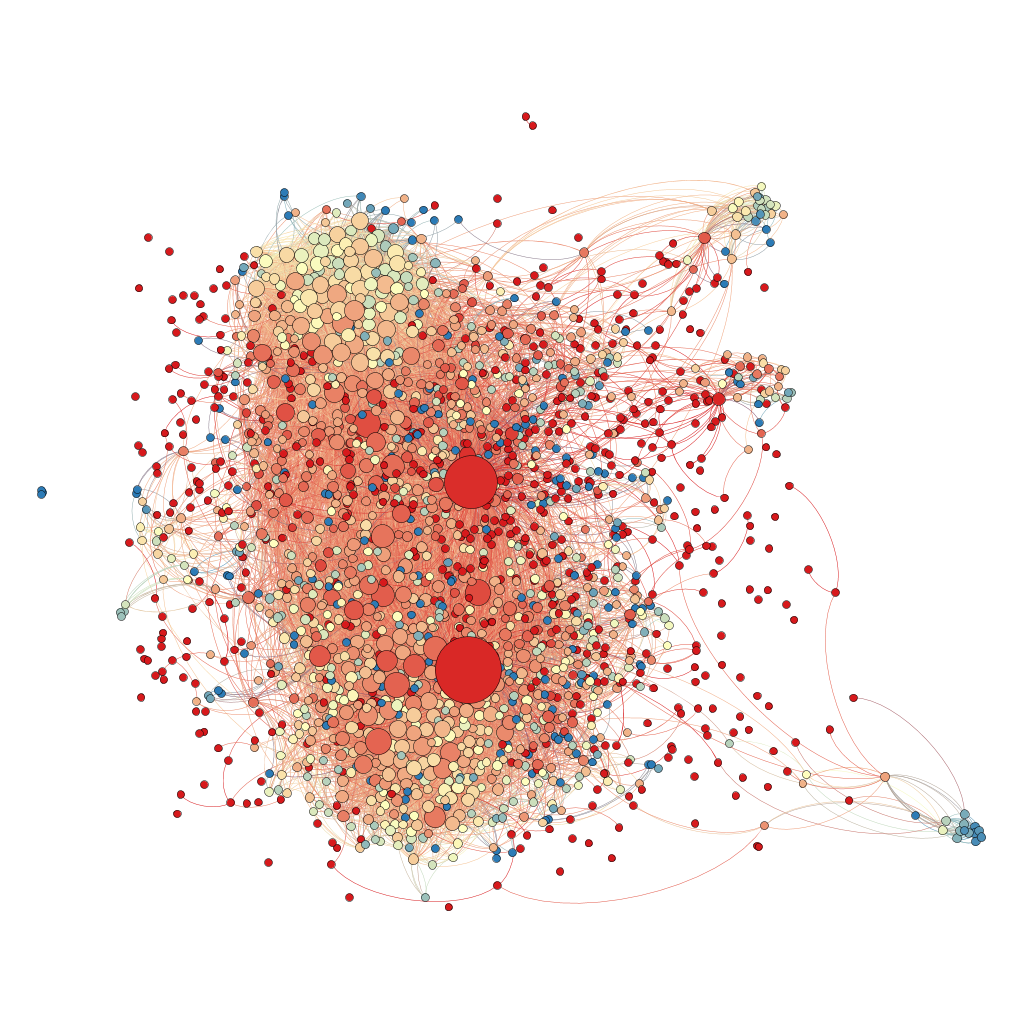
\includegraphics[scale=.25]{figs/Silicon}
% 	\caption{An example network image rendered from the Silicon Valley (Facebook) group using Gephi and the Force Atlas 2 layout algorithm.
% 	See Section~\ref{sec:gephi} for further information.}
% \label{fig:gephi}
% \begin{flushleft}\footnotesize
% Source: By the author.\
% \end{flushleft}
% \end{center}
% \end{figure}

\begin{figure}[!tbp]
	\centering
	    \subfloat[\footnotesize Without participant names.]{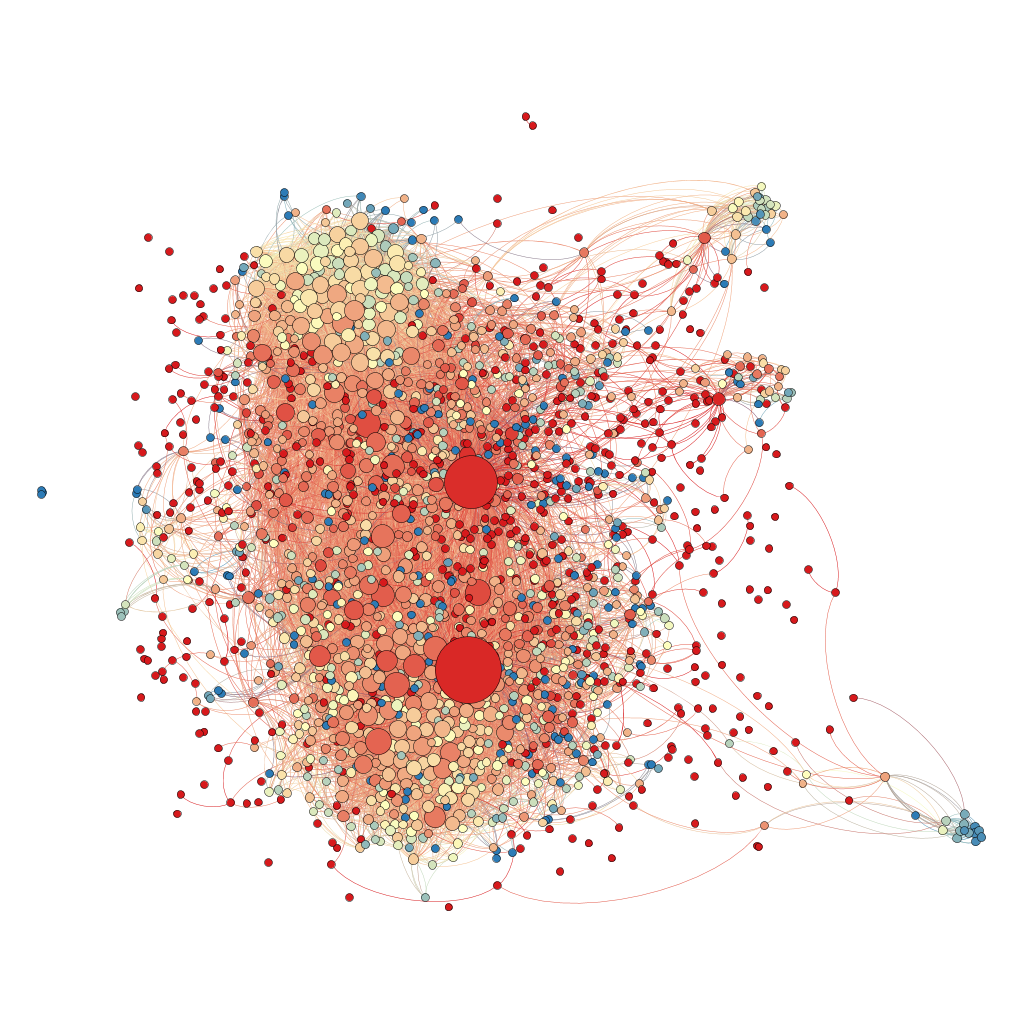
\includegraphics[width=0.45\textwidth]{figs/Silicon.png}\label{fig:f1}}
		\subfloat[\footnotesize With participant names.]{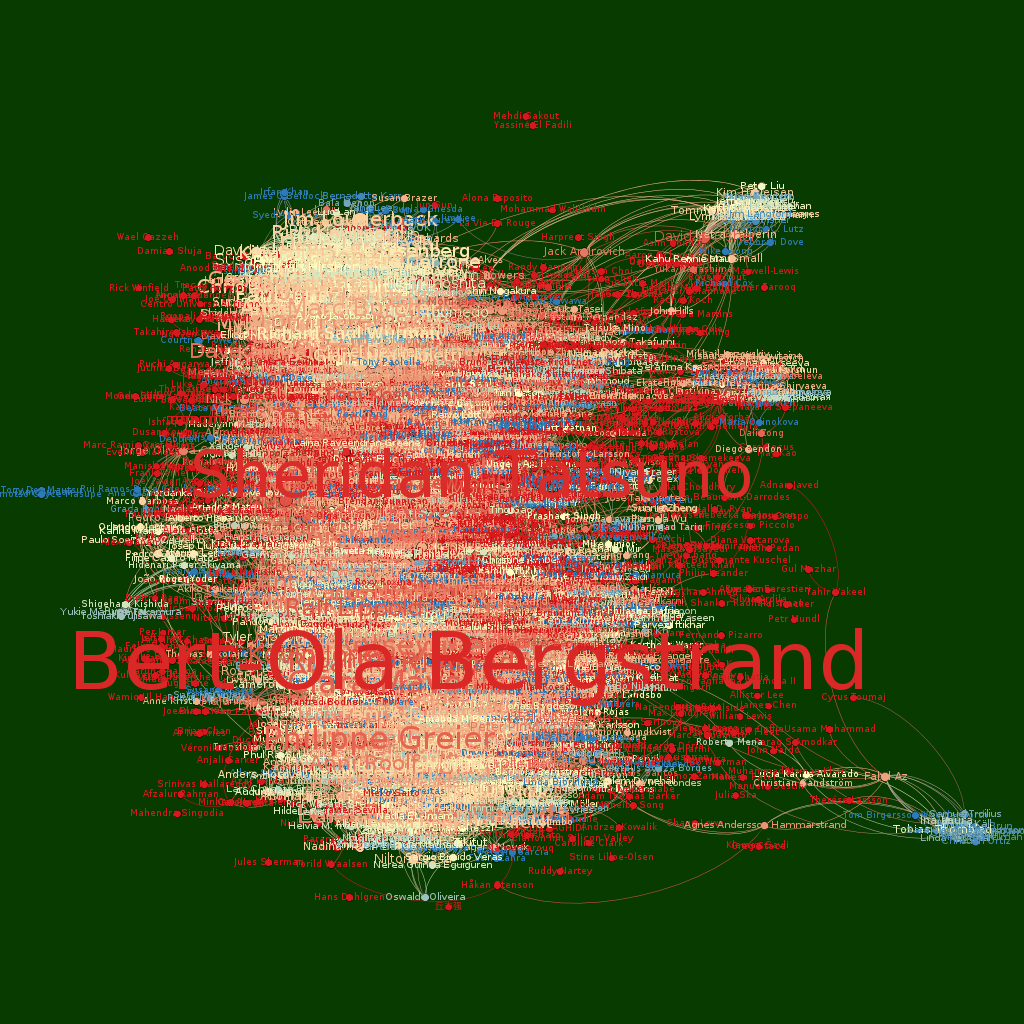
\includegraphics[width=0.45\textwidth]{figs/Silicon_nomes.png}\label{fig:f2}}
	\caption{An example network image rendered from the Silicon Valley (Facebook) group using Gephi and the Force Atlas 2 layout algorithm.
	See Section~\ref{sec:gephi} for further information.}\label{fig:gephi}
\begin{flushleft}\footnotesize
Source: By the author.\
\end{flushleft}
\end{figure}


% fb pelo gephi
	\subsection{Art by Pedro Paulo Rocha}
\section{Mega networks}
\section{Ubiquity of inequality: a simple model that explains why power laws are so frequently found in empirical data}
% arte pelo Pedro Paulo Rocha
\section{Social structures live streaming}
% telões de redes e de medidas de texto
% uso no arenaNETmundial e no ocupaGOV e outras ocasiões online
\section{Kolmogorov-Smirnov test systematic measurements}
\section{OPS: the Social Participation (OWL) Ontology}
\section{OPa: the ParticipaBR (OWL) Ontology}
\section{OntologiAA: the AA (OWL) Ontology}
\section{The Algorithmic Autoregulation software development methodology}
\section{Social Library Ontology and Social Library Vocabulary: OBS in OWL and VBS in SKOS}
% Conselhos, Foruns, Mesas Redondas, etc. Casos feitos com especialistas, casos feitos a partir de documentações
\section{Genesis of this work: complex social networks analysis by emails}
\section{United Nations Development Program consulting}
\subsection{Partnership with the Brazilian Presidency}
\subsection{Description of each product}
\section{Govern art}
\section{Ideal ideas: a physical modeling of the mind}
\section{Webpages}
% ARS, texto para pedro
\section{Collection and diffusion of information in social networks}\label{sec:colDif}
\subsection{Progressive network activation from peripherals to hubs}
\subsection{Instantaneous network activation by betweenness and closeness centralities}
\subsection{Massive tagging in Facebook and email crossposting}
\subsection{SERVDDCR online video conferences}
% processo dos periféricos aos hubs
% instantâneos pelos de maior betweenness e maior closeness
% coleta e difusão através da citação de várias pessoas e de crosspost
% SERVDDCR
\section{Anthropological physics}
The study of complex systems can be undertaken as a physics endeavor,
specially if complex networks and statistics are into play. When the complex
system is constituted by people, intriguing questions arise from diverse field such as math, ethics, and sociology. The “anthropological physics”is an approach to these scenarios that enables scientific research while resolving ethical and moral issues by an open study of the self.
	It yields a transdisciplinary practice whose relevance emanate from anthropological
and physical matters, from human constituted systems and natural laws.
A sweet spot was found in recent civil, government and academic efforts~\cite{opa,ensaio}, and has been called anthropological physics. General characteristics are:
\begin{itemize}
	\item Exposure of the researcher to the environment of interest, such as virtual social networks.
	\item Use of the annotations from the exposure, be them activity logs, friendship or interaction networks, textual contents, etc.
	\item Upon need, expansion of observations to encompass open datasets or data donated by partners.
	\item Observance of natural laws as they appear in network structures and natural language.
	\item All resources are kept as open and publicized as possible, including software, data, and writings.
\end{itemize}                                                                                                                                     
A short report the first insights regarding anthropological physics is on~\cite{anPhy}.
 
% conceitualização básica, artigo e conferências
\section{Listing of documents written, conferences attended and artistic presentations}
% rcpln
% artigos
% conferências: duas nexos+ccdc+linguística+sifiscs+ufpa+
% apresentações na SGPR, imersões, arenaNETmundial
% vivace

\end{apendicesenv}


% ----------------------------------------------------------
% Anexos
% ----------------------------------------------------------
% %% USPSC-Anexos.tex
% ---
% Inicia os anexos
% ---
\begin{anexosenv}

% Imprime uma página indicando o início dos anexos
\partanexos

% ---
\chapter{Exemplo de anexo}
% ---
Elemento opcional, que consiste em um texto ou documento não elaborado pelo autor, que serve de fundamentação, comprovação e ilustração, conforme a ABNT NBR 14724. \cite{nbr14724}.

O \textbf{ANEXO B} exemplifica como incluir um anexo em pdf.

\chapter{Acentuação (modo texto - \LaTeX)}
\begin{figure}[H]
	\begin{center}
	\caption{\label{fig_anexob}Acentuação (modo texto - \LaTeX)}
	\includegraphics[scale=1.0]{USPSC-AcentuacaoLaTeX.png} \\
	Fonte: \citeonline{comandos}
	\end{center}	
\end{figure}

\chapter{Símbolos úteis em \LaTeX}
\begin{figure}[H]
	\begin{center}
		\caption{\label{fig_anexoc}Símbolos úteis em \LaTeX}
		\includegraphics[scale=1.0]{USPSC-SimbolosUteis.png} \\
		Fonte: \citeonline{comandos}
	\end{center}	
\end{figure}


\chapter{Letras gregas em \LaTeX}
\begin{figure}[H]
	\begin{center}
		\caption{\label{fig_anexod}Letras gregas em \LaTeX}
		\includegraphics[scale=1.0]{USPSC-LetrasGregas.png} \\
		Fonte: \citeonline{comandos}
	\end{center}	
\end{figure}

\end{anexosenv}


%---------------------------------------------------------------------
% INDICE REMISSIVO
%--------------------------------------------------------------------
\phantompart
\printindex

%---------------------------------------------------------------------

\end{document}
